\documentclass[oneside]{book}
\usepackage[colorlinks,
pdfpagelabels,
pdfstartview = FitH,
bookmarksopen = true,
bookmarksnumbered = true,
linkcolor = black,
plainpages = false,
hypertexnames = false,
citecolor = black] {hyperref}
\usepackage[ngerman]{babel}
\usepackage[utf8x]{inputenc}
\usepackage[T1]{fontenc}
\usepackage{amsmath,amssymb,amstext,amsfonts}
\numberwithin{equation}{section}
\usepackage{graphicx}
\graphicspath{{./Bilder/}}

%%Kap1
\usepackage{stmaryrd} 

\title{Physik Klassen 10 und 11}
\author{Lucca Kümmerle, Patrick Müller, Josua Kugler}
\begin{document}
\begin{flushleft}

	\maketitle
	\tableofcontents
	\chapter{Klasse 10}
		\section{Mechanik (Wiederholung)}
	Die Mechanik befasst sich mit der Bewegung von Körpern, den auf diese wirkenden Kräfte und mit den zugehörigen Größen wie zum Beispiel der Energie.
	
	\subsection{Die gleichförmige Bewegung}
	Die Geschwindigkeit $ v $ ist bei der gleichförmigen Bewegung fest. Die Kurve im $ t $-$ s $-Diagramm ist eine lineare Funktion.
	% Diagramm
	Wichtig für später: Im $ t $-$ v $-Diagramm findet man die zurückgelegte Strecke $ x $ als Fläche unter dem Graphen wieder.
	Im $ t $-$ x $-Diagramm ist die Geschwindigkeit $ v $ in der Steigung (mathematisch: Ableitung) des Graphen wiederzufinden.
	
	\subsection{Der Impuls $p$}
	\paragraph{Versuch}
	% Bild
	Durch die (mehrfache) heroische Arbeit unseres Laborassistenten konnten wir folgende Beziehung zwischen Impuls $ p $, Masse $ m $ und Geschwindigkeit $ v $ nachweisen:
	\begin{itemize}
		\item Je höher die Masse $ m $ eines Körpers, desto höher der Impuls $ p $ ($ v $ konstant!).
		\item Je höher die Geschwindigkeit $ v $ eines Körpers, desto höher der Impuls $ p $ ($ m $ konstant!).
	\end{itemize}
	\paragraph{Zusammengefasst:}
	\begin{equation}
		p=m*v
	\end{equation}
	\paragraph{Weitere Eigenschaften:}
	\begin{itemize}
		\item Der Impuls $ p $ ist wie auch die Geschwindigkeit $ v $ und später auch die Kraft, eine Vektorgröße, d.h. er besitzt eine Richtung. Wenn dies von Bedeutung ist, wird zur Kenntlichmachung ein Vektorpfeil (Pfeil nach rechts) über dem Buchstaben gezeichnet.
		\item Der Impuls $ p $ ist eine Erhaltungsgröße, d.h. in einem abgeschlossenen System ist die Summe aller Impulse konstant.
	\end{itemize}
	
	\subsection{Die Kraft $F$}
	Um den Impuls $ p $ eines Körpers zu ändern, wird eine Kraft $ F $ benötigt (der konkrete mathematische Zusammenhang wird später behandelt).
	\paragraph{Beispiel:}
	Ein Spielzeugauto wird in einer realistischen Umgebung beschleunigt und dann losgelassen.
	% Bild
	Durch die Reibung zwischen Auto und Boden liegt eine Kraft $ F_{Reib} $ vor, die den Impuls des Autos abbaut, bis das Auto stoppt.
	\paragraph{Beispiel 2:}
	% Bild
	Auf Andreas wirken (im Gegensatz zu Benjamin) zwei Kräfte:\\
	Neben der Gravitationskraft $ F_G $ die ihn in Richtung Erdmittelpunkt beschleunigt, übt der Boden eine Gegenkraft $ F_{Gegen} $ mit gleicher Stärke entgegen der Gravitationskraft aus.
	\subparagraph{Folge:}
	Andreas behält seine Position bei, während er Benjamin zusieht, wie dieser nach unten beschleunigt wird.\\
	Wenn sich alle auf einen Körper wirkende Kräfte aufheben, dann liegt ein sogenanntes \underline{Kräftegleichgewicht} vor.
	
	\section{Kräfte im Raum}
	\paragraph{Wiederholung:}
	Kräfte werden durch 3 Eigenschaften charakterisiert:
	\begin{itemize}
		\item Richtung
		\item Betrag
		\item Angriffspunkt
	\end{itemize}
	Wir wissen schon, wie zwei oder mehr Kräfte miteinander verrechnet werden müssen, wenn sie (anti-)parallel zueinander sind. Im folgenden soll die Kombination von nicht parallelen Kräften untersucht werden.
	
	\subsection{Kräfteaddition}
	\paragraph{Aufgabenstellung:}
	Gegeben seien zwei Kräfte $ \vec{F_1} $ und $ \vec{F_2} $. Wie bestimmt man die daraus resultierende Gesamtkraft $ \vec{F_{Res}} $? Praktikum s. AB.
	\paragraph{Feststellung:}
	Die beiden Kräfte $ \vec{F_1} $ und $ \vec{F_2} $ bilden die Seiten eines Parallelogramms, während die resultierende Kraft $ \vec{F_{Res}} $ die Diagonale dieses Parallelogramms ist.\\
	Um zeichnerisch die Addition von zwei Kräften durchzuführen gibt es zwei Methoden:
	\paragraph{Erste Methode:}
	\begin{enumerate}
		% Bild, Text einfärben
		\item Zeichne die beiden Kraftpfeile $ \vec{F_1} $ und $ \vec{F_2} $ ein
		\item Zeichne eine parallele Gerade zu einem der Pfeile, der dann durch die Spitze des anderen Pfeils geht (bei beiden Pfeilen so machen)
		\item Der Schnittpunkt ist der Endpunkt des resultierenden Gesamtkraftpfeils $ \vec{F_{Res}} $
		\item Benutzte Pfeile wegstreichen
	\end{enumerate}
	\paragraph{Zweite Methode:}
	\begin{enumerate}
		%Bild, Text einfärben
		\item Zeichne die beiden Kraftpfeile $ \vec{F_1} $ und $ \vec{F_2} $ ein
		\item Zeichne eine parallele Gerade zu einem der Pfeile, der dann durch die Spitze des anderen Pfeils geht
		\item Miss die Länge von $ \vec{F_2} $ aus
		\item Trage die gemessene Strecke von der Spitze von $ \vec{F_1} $ ausgehend auf der Parallelen auf
		\item Der Endpunkt dieser Strecke ist die Spitze von $ \vec{F_{Res}} $
		\item Benutzte Pfeile wegstreichen
	\end{enumerate}
	
	\subsection{Die Kraftzerlegung}
	In diesem Kapitel geht es um die Zerlegung einer Kraft in zwei Kräfte entlang relevanter Richtungen
	\paragraph{Versuch:}
	%Bild
	Ziel des Versuches war, das Seil zwischen den Personen gerade zu strecken. Dies gelang fast (nur ein 10°-Knick).\\
	Erläuterungen der Verhältnisse mit Kraftpfeilen. Gravitationskraft:
	\begin{equation}
		F_G=m*g=5kg*10\dfrac{N}{kg}=50N
	\end{equation}
	Eine gleich große Kraft $ F_{Gegen} $ wird in entgegengesetzte Richtung aufgebracht. Diese Kraft wird jedoch nicht direkt aufgebracht, sondern ist das Resultat der beiden Zugkräfte von Person A und B. Diese Kräfte verlaufen entlang der gespannten Seile.\\
	Hilfskonstruktion: Gerade auf Seile einzeichnen. Dies sind sogenannte \underline{Wirkungslinien}.\\
	Um das Kräfteparallelogramm zu konstruieren, zeichne zwei Parallelen zu den Wirkungslinien, die durch die Spitze von $ F_{Gegen} $ gehen. Die zwei Kräfte entlang der Wirkungslinien gehen vom Angriffspunkt aus hin zu den Schnittpunkten aus Wirkungslinien und Parallelen.\\
	Für die Belastungskraftaufsplittung macht man das selbe, nur eben nach unten.
	
	\paragraph{Allgemein:}
	Konstruktion bei gegebenem Kraftpfeil $ \vec{F} $, der auf zwei Abschnitte an einem Angriffspunkt wirkt:
	% Bild/Skizze
	\begin{enumerate}
		\item Zeichne die Wirkungslinien entlang der Abschnitte ein
		\item Zeichne Parallelen zu den Wirkungslinien durch die Spitze des Kraftpfeils $ \vec{F} $
		\item Kraftkomponenten $ \vec{F_1} $ und $ \vec{F_2} $ verlaufen vom Angriffspunkt aus hin zu den Schnittpunkten aus Wirkungslinien und Parallelen
	\end{enumerate}
	\paragraph{Zurück zum Einstiegsbeispiel:}
	% Bild/Skizze
	\subparagraph{Betrachtung:}
	Das Kräfteparallelogramm ist (wenn $ \vec{F_1} $ und $ \vec{F_2} $ gleichgroß sind) nicht nur ein Parallelogramm, sondern auch eine Raute.
	% Bild/Skizze
	\begin{subequations}
		\begin{align}
			\beta &= \dfrac{\alpha}{2}\\
			\sin\beta &= \dfrac{\dfrac{1}{2}\vec{F_{Res}}}{\vec{F_2}}\\
			\vec{F_2} &= \dfrac{\dfrac{1}{2}\vec{F_{Res}}}{\sin\beta}\\
			& \approx 278N
		\end{align}
	\end{subequations}
	
	\subsubsection{Kräfte an einem Hang}
	Die Kraftzerlegung eignet sich auch dazu, beispielsweise die Gravitationskraft, die auf einen Körper wirkt an einem, Hang in bewegungsrelevante Kräfte zu zerteilen.
	% Bild/Skizze
	\begin{description}
		\item[$ F_H $] ist die sogenannte Hangabtriebskraft und beschreibt die beschleunigende Kraft, die auf den Körper entlang des Hangs wirkt.
		\item[$ F_N $] ist die Normkraft und gibt an, wie stark der Körper auf die Oberfläche des Hangs drückt.
	\end{description}
	-->AB
	\paragraph{Es gilt also:}
	% Bild/Skizze
	\begin{equation}
		\dfrac{F_H}{F_G} = \dfrac{h}{s} = \sin\alpha
	\end{equation}
	Demzufolge kann man die Hangabtriebskraft aus der Gravitationskraft und dem Hangwinkel wie folgt berechnen:
	\begin{equation}
	F_H = F_G*\sin\alpha
	\end{equation}
	Analog folgt für die zu $ F_H $ senkrecht stehende Normkraft $ F_N $:
	\begin{equation}
	F_N = F_G*\cos\alpha
	\end{equation}
	$ F_N $ ist mit einem Faktor ($ \mu_t $) mit der Reibung verbunden ($ t $ ist entweder $ Haft $, $ Gleit $ oder $ Roll $). Die Haftreibung ist beispielsweise:
	\begin{align}
		F_{Haft} &= \mu_{Haft}*F_N\\
		&= \mu_{Haft}*F_G*\cos\alpha
	\end{align}
	Der Haftreibungskoeffizient ist abhängig davon, welche Materialien miteinander in Kontakt stehen.
	% Bild/Skizze
	Um den Haftreibungskoeffizienten $ \mu_{Haft} $ in dem praxisnahen Fall Taschenrechner-Tagebuch zu untersuchen wird das Tagebuch immer stärker geneigt, bis der Taschenrechner auf dem Tagebuch herunterrutscht. Unter de, gemessenen Winkel ist dann die \underline{Hangabtriebskraft} $ F_H $ größer als die \underline{Reibungskraft} $ F_{Reib} $.\\
	\emph{Messung:} $ \alpha = 27° $
	\begin{align}
		F_H &\geqq F_{Reib}\\
		F_G*\sin\alpha &\geqq \mu_{Haft}*F_G*\cos\alpha\ && |:(F_G*\cos\alpha)\\
		\dfrac{F_G*\sin\alpha}{F_G*\cos\alpha} &\geqq \mu_{Haft}\\
		\tan\alpha &\geqq \mu_{Haft}\\
		\nonumber\\
		\Rightarrow\hspace{0.5cm} \mu_{Haft} &\leqq 0,51 \quad \text{(Einheitenlos)}
	\end{align}
	
	\subsection{Die gleichmäßig beschleunigte Bewegung}
	\paragraph{Alt:}
	\begin{itemize}
		\item Gleichförmige Bewegung
		\item Geschwindigkeit $ v $ ist konstant
		\item $ t $-$ s $-Diagramm ist eine lineare Funktion
	\end{itemize}
	\paragraph{Neu:}
	\begin{itemize}
		\item Gleichmäßig beschleunigte Bewegung
		\item Geschwindigkeit $ v $ nimmt konstant zu
		\item $ t $-$ v $-Diagramm ist eine lineare Funktion
	\end{itemize}

	\subsection{Die Newtonschen Gesetze}
	\subsubsection{Erstes Newtonsches Gesetz}
	\paragraph{Gedankenexperiment:}
	% Bild
	Die Voyager-Sonde fliegt durch das Weltall. Sei die Geschwindigkeit zum Zeitpunkt $ t=0s $ $ v=500\frac{m}{s} $. Auf die Sonde wirkt keine Kraft, wie groß ist ihre Geschwindigkeit bei $ t=5s $?
	\subparagraph{Antwort:}
	Noch immer $ v=500\frac{m}{s} $, da keine beschleunigende Kraft wirkt.
	\paragraph{Erstes Newtonsches Gesetz:}
	Wirkt auf einen Körper keine Kraft, so bleibt sein Bewegungszustand (und somit sein Impuls) erhalten.
	
	\subsubsection{Zweites Newtonsches Gesetz}
	\paragraph{Gedankenexperiment 2:}
	% Bild
	Überlegungen zum Bremsvorganf des Einkaufswagens: Es hängen folgende Größen miteinander zusammen: Kraft $ F $, Beschleunigung $ a $ und Masse $ m $.\\
	Vermutungen:
	\begin{itemize}
		\item bei konstanter Masse $ m $: Je größer $ a $ sein soll, desto größer muss $ F $ sein
		\item bei konstanter Kraft $ F $: Je größer $ m $, desto kleiner $ a $
		\item bei konstanter Beschleunigung $ a $: Je größer $ m $, desto größer $ F $
	\end{itemize}
	Bei der dritten Versuchsreihe vermuten wir eine proportionale Beziehung zwischen beschleunigender Kraft $ F $ und Gesamtmasse $ m $, d.h. dass, wenn der Quotient aus Kraft und Gesamtmasse konstant ist ($ \frac{F}{m} $), die Beschleunigung auch konstant bleibt. Dies wurde durch die Untersuchung qualitativ bestätigt.
	\paragraph{Zusammenfassung:}
	\begin{align}
		\left.
		\begin{array}{c}
		F \sim a \quad\text{(m const.)}\\
		\\
		F \sim m \; \quad\text{(a const.)}
		\end{array}
		\right\}
		F \sim m*a
	\end{align}
	Um eine Formel daraus zu machen fehlt eine Proportionalitätskonstante. Nennen wir sie $c$. Die Formel lautet dann also:
	\begin{align}
		F &= c*m*a\\
		c &= \dfrac{F}{m*a}
	\end{align}
	Bestimmung von $ c $ mithilfe der Tabelle (mit $ F $ in $ N $, $ m $ in $ kg $ und $ a $ in $ \frac{m}{s^2} $)
	\begin{equation}
		c = \dfrac{0,02N}{0,206kg*0,09\dfrac{m}{s^2}} \approx 1,08
	\end{equation}
	Bei einer genauen Untersuchung (mit genau bestimmtem $ g $) ergibt sich $ c=1 $. Die Grundgleichung der Mechanik (=Newtons zweites Gesetz) lautet also:
	\begin{equation}
		F = m*a
	\end{equation}
	
	\subsubsection{Drittes Newtonsches Gesetz}
	\paragraph{Versuch:}
	% Bild
	\subparagraph{Beobachtung:}
	Wirft Person $ A $ den Ball $ B $ nach rechts, dann wird Person $ A $ nach links beschleunigt.
	\subparagraph{Folgerung:}
	Auch auf Person $ A $ wird beim Wurf eine Kraft in entgegengesetzte Richtung aufgebracht. Dies ist das dritte Newtonsche Gesetz.
	\paragraph{Drittes Newtonsches Gesetz:}
	Übt ein Körper $ A $ eine Kraft $ \vec{F_{AB}} $ auf einen Körper $ B $ aus, so erfährt Körper A ebenfalls eine Kraft $ \vec{F_{BA}} $ gleicher Größe, aber entgegengesetzter Richtung. Es gilt also:
	\begin{align}
		\mid\vec{F_{AB}}\mid &= \ \ \mid\vec{F_{BA}}\mid\\
		\vec{F_{AB}} &= -\vec{F_{BA}}
	\end{align}
	Wird eine Kraft $ F_{AB} $ auf einen Körper B angewandt und dauert dies die Zeit $ \Delta t $, dann folgt:
	\begin{align}
		F_{AB}*\Delta t &= m_B*a*\Delta t\\
		&= m_B*\Delta v\\
		&= \Delta p_B
	\end{align}
	Dies ist also die Impulsänderung. Wenn man Newton 3 analog für die andere Seite anwendet, erhält man:
	\begin{equation}
		\Delta p_B = -\Delta p_A
	\end{equation}
	Wenn man beide Impulsänderungen $ \Delta p_A $ und $ \Delta p_B $ addiert (also alle Impulsänderungen zusammenfasst), dann kommt heraus:
	\begin{equation}
		\Delta p_B+\Delta p_A = 0
	\end{equation}
	D.h. der Gesamtimpuls dieses abgeschlossenen Systems bleibt erhalten.
	
	\subsection{Die überlagerte Bewegung}
	Aus dem Übungsblatt ``Übungen zur Grundgleichung der Mechanik'' haben wir in f) erarbeitet, dass wenn eine Bewegung die Summe aus verschiedenen Bewegungsarten ist (im Beispiel: gleichförmige und gleichmäßig beschleunigte Bewegung), man die Bewegungsarten separat berechnen kann und anschließend erst zusammenaddieren kann.
	\paragraph{Teil 2:}
	Bewegungen müssen nicht nur entlang einer Raumachse stattfinden (z.B. schräger Wurf). Wenn die Bewegung in eine Raumrichtung die Bewegung in eine andere Raumrichtung nicht beeinflusst, dann kann man die Ortsverläufe in den einzelnen Raumrichtungen zu verschiedenen Zeitpunkten $ t $ separat berechnen und die errechneten Koordinaten in einer Ortsverlaufskurve zusammenfassen.
	
	\subsection{Erhaltungssätze}
	\subsubsection{Der Energieerhaltungssatz}
	Aus den Hebelgesetzen bzw. Versuchen mit dem Flaschenzug haben wir herausgefunden:
	% Bild
	\begin{align}
		\intertext{Was man an Weg spart, muss man an Kraft ausgleichen. Es gilt also:}
		F_1*s_1=F_2*s_2
	\end{align}
	Das Produkt aus beiden ist erhalten. Hinter diesem Produkt steht als Größe die \underline{Energie} $ E $.\\
	\emph{DIE ENERGIE IST ERHALTEN}\\
	Wird die Masse hochgezogen, dann wird die Energie, die die Masse gewinnt, als Höhenenergie bzw. potentielle Energie $ E_{pot} $ bezeichnet.
	\begin{equation}
		E_{pot} = F*s = F_G*h = m*g*h
	\end{equation}
	
	\subsubsection{Die kinetische Energie}
	\paragraph{Versuch:}
	Eine Kugel rollt einen Hang hinab. Sie verliert an potentieller Energie. Die Gesamtenergie eines Systems ist aber konstant.
	\paragraph{Folgerung:}
	Die potentielle Energie wurde in eine andere Energie umgewandelt, nämlich in Bewegungsenergie $ E_{kin} $ (auch kinetische Energie genannt).
	% Bild/Skizze
	\paragraph{Überlegung:}
	Je höher die Geschwindigkeit $ v $, desto größer die zugehörige kinetische Energie $ E_{kin} $.
	% (Bild)
	\paragraph{Gedankenexperiment:} Eine Kugel wird aus der Höhe $ h $ auf den Boden fallen gelassen. Die Höhenenergie $ E_{pot} $, die umgewandelt ist, beträgt:
	\begin{equation}
		E_{pot} = m*g*h
	\end{equation}
	Die Geschwindigkeit $ v $, die die Kugel unten ankommend hat, beträgt mithilfe der Formel für gleichmäßig beschleunigte Bewegung:
	\begin{align}
		h = s &= \dfrac{1}{2}*a*t^2\\
		&= \dfrac{1}{2}*\dfrac{a*t^2*a}{a}\\
		&= \dfrac{1}{2}*\dfrac{a^2*t^2}{a} && |v=a*t\\
		&= \dfrac{1}{2}*\dfrac{v^2}{a}\\
		v &= \sqrt{2*a*s}
	\end{align}
	Ist die Kugel unten angekommen, dann wurde die gesamte potentielle Energie in kinetische Energie umgewandelt:
	\begin{align}
		E_{pot} &= E_{kin}\\
		m*g*h &\stackrel{(\wedge)}{=} m*g*\dfrac{1}{2}*\dfrac{v^2}{a}\\
		&\stackrel{g=a}{=} m*\dfrac{1}{2}*v^2\\
		\nonumber\\
		\Rightarrow\hspace{0.5cm} E_{kin} &= \dfrac{1}{2}*m*v^2
	\end{align}
	
	\subsubsection{Die Spannenergie}
	Versuch mit Federn mit bestimmten Eigenschaften (Hookesche Federn)... s. Praktikum.
	\paragraph{Ergebnis:}
	$ F $ ist proportional zur Streckung $ s $. Der Proportionalitätsfaktor ist die sogenannte Federhärte $ D $.
	% Diagramm
	\begin{align}
		F &= D*s\\
		\nonumber\\
		[D] = \left[\dfrac{F}{s}\right] &= \dfrac{1N}{1m}
	\end{align}
	\paragraph{Vergleich:}
	Ein Massestück wird von $ h=0 $ bis $ h=h_1 $ angehoben. Wie hängen $ F $, $ \Delta h $ und $ E $ zusammen?
	% Diagramm
	\begin{align}
		E &= F*\Delta h\\
		&= m*g*\Delta h
	\end{align}
	$ E $ ist die Fläche unter der Kurve.
	\paragraph{Jetzt:}
	Wo verbirgt sich die Spannenergie $ E_{spann} $ im $ s $-$ F $-Diagramm der Feder?
	% Diagramm
	\begin{align}
		E_{spann} &= \dfrac{1}{2}*F*s\\
		E_{spann} &= \dfrac{1}{2}*D*s^2
	\end{align}
	
	\subsection{Die Impulserhaltung}
	\subsubsection{Der vollständig inelastische Stoß}
	Beim vollständig inelastischen Stoß kollidieren zwei Körper miteinander und bewegen sich nach dem Stoß gemeinsam mit der gleichen Geschwindigkeit weiter.
	\paragraph{Zu erwartende Formeln:}
	\begin{align}
		\intertext{Impuls:}
		p_1 + p_2 &= p'\\
		m_1*v_1+m_2*v_2 &= m'*v'\\
		&= (m_1+m_2)*v'\\
		\intertext{Energie:}
		E_{kin_{1}}+E_{kin_{2}} &= E'_{kin}\\
		\dfrac{1}{2}*m_1*{v_1}^2+\dfrac{1}{2}*m_2*{v_2}^2 &= \dfrac{1}{2}*m'*{v'}^2\\
		&= \dfrac{1}{2}*(m_1+m_2)*{v'}^2
	\end{align}
	Die kinetische Energie scheint bei den durchgeführten Versuchen nicht erhalten zu sein. Das lässt sich jedoch durch die, für die Verformung (und Erwärmung) der Knetmasse benötigte Energie erklären. Kurz gesagt: Ein Teil der kinetischen Energie wird nicht als kinetische Energie erhalten, sondern zu einer anderen Form von Energie umgewandelt. Deshalb:
	\begin{align}
		\intertext{Nicht:}
		E_{kin_{1}}+E_{kin_{2}} &= E'_{kin}\\
		\intertext{Sondern:}
		E_{kin_{1}}+E_{kin_{2}} &= E'_{kin}+U\\
		U &= \dfrac{1}{2}*\dfrac{m_1*m_2}{m_1+m_2}*(v_1-v_2)^2
	\end{align}
	\paragraph{Merke:}
	Die zentrale Formel für die Impulse beim vollständig inelastischen Stoß lautet:
	\begin{align}
		p_1 + p_2 &= p'\\
		m_1*v_1+m_2*v_2 &= m'*v'\\
		m_1*v_1+m_2*v_2 &= (m_1+m_2)*v'\\
		\intertext{bzw. nach $ v' $ aufgelöst:}
		v' &= \dfrac{m_1*v_1+m_2*v_2}{m_1+m_2}
	\end{align}
	\paragraph{Wichtig:}
	$ v $ ist eine Vektorgröße. In den meisten Aufgabenstellungen wird dabei die Bewegung in eine Richtung (z.B. in $ x $-Richtung) untersucht. Daher kann $ v_1 $, $ v_2 $ und $ v' $ auch negativ sein.
	
	\emph{Hier fehlen die Blätter dazwischen drinnen!!!}\\
	\emph{Z.B. der vollständig elastische Stoß fehlt komplett!!!}
	
	\subsection{Alltagsbeispiel: Autocrash}
	Kollidiert ein Auto mit einer Wand, so wird sein Impuls $ p $ vollständig abgebaut. Es gilt:
	\begin{align}
		\Delta p &= m*\Delta v\\
		&= F*\Delta t
	\end{align}
	Diese Formeln gelten unter der Annahme, dass die Kraft konstant ist, d.h. dass im gleichen Zeitfenster die gleiche Menge an Impuls abgebaut wird. Wird der Impuls jedoch nicht gleichmäßig abgebaut, so muss man die Impulsänderungen Zeitintervallen zuordnen und daraus die momentane Kraft berechnen.
	\begin{equation}
		F = \dfrac{\Delta p}{\Delta t}
	\end{equation}
	Lassen wir die Zeitintervalle ganz klein werden, dann folgt:
	\begin{equation}
		F(t) = \lim\limits_{\Delta t\to 0}\dfrac{\Delta p}{\Delta t} = p'(t)
	\end{equation}
	
	\section{Mechanik der Kreis- und Rotationsbewegung}
	\subsection{Die Kreisbewegung}
	\paragraph{Versuch:}
	% Bild/Skizze
	\subparagraph{Beobachtung:}
	Der Punkt $ P $ bewegt sich mit \underline{konstanter} Geschwindigkeit auf einer Kreisbahn. In diesem Fall spricht man von der \underline{gleichförmigen Kreisbewegung}.\\
	\paragraph{Größen zur Beschreibung der Bewegung:}
	\begin{description}
		\item[Radius] $ r $
		\item[Winkel] $ \alpha $ oder (s.u.) $ \varphi $
		\item[Bogenstrecke] $ b $
		\item[Kreisbahngeschwindigkeit] $ v $
		\item[Zeit] $ t $
		\item[Periodendauer] $ T $ (Zeit für eine volle Umkreisung)
		\item[Frequenz] $ f $
		\item[Kreisfrequenz] $ \omega $
		\item[Kraft] $ F $
		\item[Beschleunigung] $ a $
	\end{description}
	
	\subsection{Das Bogenmaß $\varphi$}
	Um beispielsweise den Kreisbogen $ b $ zu berechnen muss man bei gegebenem Winkel $ \alpha $ wie folgt rechnen:
	\begin{equation}
		b = \dfrac{\alpha}{360°}*2*\pi*r
	\end{equation}
	Jetzt: \underline{definiere} den Winkel $ \varphi $ so, dass der Term für $ b $ am Ende nicht mehr $ 360° $ und $ 2*\pi $ enthält:
	\begin{align}
		b &= \dfrac{\varphi}{2*\pi}*2*\pi*r\\
		\Rightarrow\hspace{0.5cm} b &= \varphi*r
	\end{align}
	Findet z.B. eine volle Umdrehung statt (in Grad wäre das $ 360° $), dann folgt für das Bogenmaß $ \varphi $:
	\begin{align}
		\varphi &= \dfrac{b}{r} = \dfrac{\dfrac{360°}{360°}*2*\pi*r}{r}\\
		\nonumber\\
		&= 2*\pi
	\end{align}
	Die Einheit des Bogenmaßes ist der Radiant und ist dimensionslos. Der Vorteil des Bogenmaßes wird in den kommenden Übungen ersichtlich.
	
	\subsection{Grundlegende wichtige Gleichungen für die Kreisbewegung}
	\begin{align}
		\intertext{Bogenmaß}
		\varphi &= \dfrac{b}{r}\\
		\nonumber\\
		\intertext{Umwandlung zwischen Grad und Radiant}
		\dfrac{\varphi}{2*\pi} &= \dfrac{\alpha}{360°} \quad \Longleftrightarrow \quad \alpha = 180°*\dfrac{\varphi}{\pi} \quad \Longleftrightarrow \quad \varphi = \pi*\dfrac{\alpha}{180°}\\
		\nonumber\\
		\intertext{Kreisbahngeschwindigkeit}
		v &= \dfrac{2*\pi*r}{T}\\
		\nonumber\\
		\intertext{Umlaufzeit bzw. Periodendauer}
		T &= \dfrac{2*\pi*r}{v}\\
		\nonumber\\
		\intertext{Frequenz bzw. Umdrehungen pro Zeiteinheit}
		f &= \dfrac{1}{T}\\
		\nonumber\\
		\intertext{Winkelgeschwindigkeit bzw. Winkel pro Zeiteinheit}
		\omega &= \dfrac{2*\pi}{T} = 2*\pi*f = \dfrac{v}{r}\\
		\nonumber\\
		\intertext{Gleichförmige Kreisbewegung:}
		\varphi(t) &= \omega*t
	\end{align}
	
	\subsection{Die Zentripetalkraft}
	\paragraph{Versuch:}
	Eine Kugel rollt zunächst geradlinig durch den Raum. Durch Stöße soll sie auf eine Kreisbahn gebracht werden.
	% Bild\Skizze
	Um die Änderung der Bewegungsrichtung herbeizuführen braucht es eine Impulsänderung $ \Delta \vec{p} $, die wiederum durch Einwirkung einer Kraft $ \vec{F} $ während einer Zeitspanne $ \Delta t $ erbracht wird. Die Kräfte wirken zu jedem Zeitpunkt auf den Mittelpunkt des Kreisbogens. Daher wird die für diese Bewegung verantwortliche Kraft \underline{Zentripetalkraft} $ F_{ZP} $ (lat. \textit{centrum} = Mitte, lat. \textit{petere} = streben) bezeichnet.
	\paragraph{Frage:}
	Wovon hängt die aufzubringende Kraft ab?
	\begin{itemize}
		\item Masse des Körpers $ m $
		\item Radius $ r $
		\item Winkelgeschwindigkeit $ \omega $
	\end{itemize}
	\paragraph{Ergebnis:}
	\begin{itemize}
		\item Je größer $ m $, desto größer $ F $
		\item Je größer $ r $, desto größer $ F $
		\item Je größer $ \omega $, desto größer $ F $
	\end{itemize}
	\paragraph{Vorbemerkung zu weiteren Aufgaben der ZP:}
	Beispiel Kavalierstart (Gaspedal bei Start voll durchgedrückt):\\
	Effekt: Reifen drehen durch.\\
	Ursache: Die Kraft, die vom Motor aus auf das Rad übertragen wird, ist viel größer als die Haftreibungskraft, die dafür sorgt, dass die Kraft von den Reifen auf die Straße übertragen wird und somit das Auto beschleunigt wird. sobald die Reifen durchdrehen, ist die Gleitreibungskraft die Kraft, die die Beschleunigung des Wagens bewerkstelligt. Da $ \mu_{Gleit} < \mu_{Haft} $ ist, ist die Beschleunigung des Wagens kleiner, als im Fall bei haftenden Reifen.
	
	\subsection{Inertialsysteme und Newton 1}
	\paragraph{Wir wissen:}
	2. Newtonsches Gesetz: $ F = m*a $. Ist dann Newton 1 (``wenn keine Kraft, dann keine Änderung des Bewegungszustandes (also Beschleunigung 0?)'') in Anbetracht von Newton 2 überflüssig?
	\paragraph{Newton 1 sagt mehr:} Es legt Bezugssysteme (d.h. das Koordinatensystem, in dem die Bewegung von Körpern beschrieben wird) fest, die mit der Newtonschen Mechanik beschrieben werden. Insbesondere werden dadurch Koordinatensysteme von der Newtonschen Mechanik ausgeschlossen, deren Ursprung sich im Raum beschleunigt.
	
	\subsection{Die Rotationsenergie und das Trägheitsmoment}
	\paragraph{Versuch:}
	Zwei Konservendosen gleicher Masse $ m $ aber verschiedener Inhaltszusammensetzung (flüssige Suppe vs. ``fester'' Eintopf) werden auf einem Hang gleichzeitig rollen gelassen.
	\subparagraph{Beobachtung:}
	Die Suppe kommt zuerst unten an.
	% Bild/Skizze
	\subparagraph{Erklärung:}
	Bei der Dose mit dem festen Inhalt muss der Inhalt mitgedreht werden. Hierfür ist Energie notwendig (die Rotationsenergie $ E_{rot} $) die dann eben nicht mehr für die lineare Bewegung (gekoppelt an die kinetische Energie $ E_{kin} $) zur Verfügung steht.\\
	D.h. näherungsweise beträgt die Gesamtenergie der Dosen:
	\begin{align}
		E_{ges, fest} &= E_{kin}+E_{rot}\\
		E_{ges, fl\textit{\"u}ssig} &= E_{kin}+\underbrace{E_{rot}}_{\substack{\approx \ 0J\text{, da}\\\text{Flüssigkeit} \\ \text{nicht mit-}\\\text{rotiert}}} = E_{kin}
	\end{align}
	Ziel des Kapitels ist es nun, einen eleganten Ausdruck zu finden, mit dem sich die Rotationsenergie berechnen lässt.
	% Bild/Skizze
	Die Rotationsenergie ist nichts anderes als die Summe der kinetischen Energien der einzelnen Massenteile des Körpers. Es gilt also bei $ n $ Massenteilen im Körper:
	\begin{align}
		E_{rot} &= E_{kin_1}+E_{kin_2}+E_{kin_3}+...+E_{kin_n}\\
		&= \dfrac{1}{2}*m_1*v_1^2+\dfrac{1}{2}*m_2*v_2^2+\dfrac{1}{2}*m_3*v_3^2+...+\dfrac{1}{2}*m_n*v_n^2
	\end{align}
	\paragraph{Problem:}
	Die Berechnung der Geschwindigkeiten erweist sich als zeitraubend, da, wenn sich die Dose auch nur etwas schneller dreht, die Geschwindigkeit für jedes Massenteil neu berechnet werden muss.
	\paragraph{Lösung:}
	Ersetze die Geschwindigkeitsterme durch die Winkelgeschwindigkeit $ \omega $:
	\begin{align}
		E_{rot} &= \dfrac{m_1*v_1^2}{2}+\dfrac{m_2*v_2^2}{2}+\dfrac{m_3*v_3^2}{2}+...+\dfrac{m_n*v_n^2}{2}\\
		\nonumber\\
		&= \dfrac{m_1*r_1^2*v_1^2}{2*r_1^2}+\dfrac{m_2*r_2^2*v_2^2}{2*r_2^2}+\dfrac{m_3*r_3^2*v_3^2}{2*r_3^2}+...+\dfrac{m_n*r_n^2*v_n^2}{2*r_n^2}\\
		\nonumber\\
		&= \dfrac{m_1*r_1^2}{2}*\dfrac{v_1^2}{r_1^2}+\dfrac{m_2*r_2^2}{2}*\dfrac{v_2^2}{r_2^2}+\dfrac{m_3*r_3^2}{2}*\dfrac{v_3^2}{r_3^2}+...+\dfrac{m_n*r_n^2}{2}*\dfrac{v_n^2}{r_n^2}\\
		\nonumber\\
		&= \dfrac{1}{2}*(m_1*r_1^2*\omega^2+m_2*r_2^2*\omega^2+m_3*r_3^2*\omega^2+...+m_n*r_n^2*\omega^2)\\
		&= \dfrac{1}{2}*\underbrace{(m_1*r_1^2+m_2*r_2^2+m_3*r_3^2+...+m_n*r_n^2)}*\omega^2\\
		&= \dfrac{1}{2}* \hspace{3.8cm} J \hspace{3.8cm}*\omega^2
	\end{align}
	$J$ ist das sogenannte Trägheitsmoment. Es hat die Einheit $ kg*m^2 $. Wenn in einer Aufgabenstellung die Masse und Radien gegeben sind, dann rechnet man $J$ nach der Formel
	\begin{equation}
		J = m_1*r_1^2+m_2*r_2^2+m_3*r_3^2+...+m_n*r_n^2
	\end{equation}
	aus. Ansonsten haben aufopferungsvolle Physiker und Mathematiker für bekannte geometrische Objekte (z.B. Zylinder) ihr Blut vergossen, um eine kompakte Formel bereitzustellen. Zum Beispiel:
	\begin{equation}
		J_{Zylinder} = \dfrac{1}{2}*m*r^2
	\end{equation}
	(hierbei ist angenommen, dass die Masse im Zylinder gleichförmig verteilt ist. Mit $ r $ ist der Radius an den äußeren Rand des Zylinders gemeint.)
	\paragraph{Daraus folgt:}
	\begin{itemize}
		\item Je größer $ r $, desto größer $ J $ \quad (bei gleichbleibendem $ m $)
		\item Je größer $ m $, desto größer $ J $ \quad (bei gleichbleibendem $ r $)
	\end{itemize}
	\paragraph{Zusammenfassung:}
	Die Rotationsenergie $ E_{rot} $ berechnet sich zu
	\begin{align}
		E_{rot} &= \dfrac{1}{2}*J*\omega^2
		\intertext{wobei J das sogenannte Trägheitmoment ist und sich entweder über}
		J &= m_1*r_1^2+m_2*r_2^2+m_3*r_3^2+...+m_n*r_n^2
		\intertext{oder über eine angegebene Formel berechnet, wie z.B. beim Zylinder:}
		J_{Zylinder} &= \dfrac{1}{2}*m*r^2
		\intertext{Rollt ein Körper über eine Oberfläche hinweg, dann hat er sowohl kinetische Energie $ E_{kin} $ aus der linearen Bewegung als auch Rotationsenergie $ E_{rot} $ aus der Rotation. Es gilt dann:}
		E_{Ges} &= E_{rot}+E_{kin}\\
		&= \frac{1}{2}*J*\omega^2+\frac{1}{2}*m*v^2
		\intertext{$ \omega $ ist mit $ v $ dann über den Rollradius $ r_{roll} $ verbunden:}
		\omega &= \dfrac{v}{r_{roll}}
	\end{align}
	
	\subsection{Der Drehimpuls $ L $}
	Aus der Analogietabelle haben wir hergeleitet, dass das Analogon zum Impuls $ p $ der linearen Bewegung
	\begin{equation}
		p = m*v
	\end{equation}
	der Drehimpuls $ L $ der Rotationsbewegung
	\begin{equation}
		L = J*\omega
	\end{equation}
	ist. Im folgenden Versuch soll eine weitere Eigenschaft und auch Analogie zwischen Impuls und Drehimpuls ergründet werden.
	\paragraph{Versuch:}
	% Bild/Skizze
	Wenn die Person während der Rotationsbewegung die Arme anzieht, dann wird das Trägheitsmoment $ J $ kleiner. Jedoch sah man, dass die Rotationsgeschwindigkeit $ \omega $ währenddessen anstieg.
	\paragraph{Folgerung:}
	Der Drehimpuls $ L $ ist wie der Impuls $ p $ eine Erhaltungsgröße.
	
	\paragraph{Der Fall einer Katze:}
	\begin{enumerate}
		\item Katze schaut nach unten. Gesamtdrehimpuls $ L_{Ges} = 0 $.
		\item Katze zieht Vorderbeine an, streckt Hinterbeine aus $ \to \ \ J_{vorne} $ klein, $ J_{hinten} $ groß.
		% Bild/Skizze
		\item Vorder- und Hinterkörper drehen sich in entgegengesetzte Richtungen (zur Erhaltung des Gesamtdrehimpulses $ L_{Ges} $). Da $ J_{vorne} < J_{hinten} $ folgt $ \omega_{vorne} > \omega_{hinten} $.
		% Bild/Skizze
		\item Katze streckt Vorderbeine aus, zieht Hinterbeine an $ \to \ \ J_{vorne} > J_{hinten} $
		\item Katze dreht sich. $ \omega_{hinten} > \omega_{vorne} $ (mit entgegengesetztem Vorzeichen).
		% Bild/Skizze
		\item Katze streckt Extremitäten aus $ \to $ Bremsweg $ s $ wird größer\\
		$ \to $ $ a $ wird kleiner $ \to $ belastende Kraft $ F $ wird kleiner.
	\end{enumerate}
	\paragraph{Die Richtung des Drehimpulses:}
	Betrachte sich drehendes Rad (Masse auf Radius):
	% Bild/Skizze
	Berechne den Drehimpuls $ L $ (nehme an, dass sich nur ein einziges Massenstück auf dem Radius befindet):
	\begin{align}
		L &= \quad J\hspace{0.34cm}*\hspace{0.34cm}\omega\\
		&= \overbrace{m*r^2}*\overbrace{\dfrac{v}{r}}\\
		&= m*r*v\\
		&= \underbrace{m*v}*r\\
		&= \hspace{0.34cm}p\hspace{0.15cm}*\hspace{0.15cm}r
	\end{align}
	Den Drehimpuls eines Massenteilchens kann man also auch beschreiben als das (Vektor-) Produkt aus dem Impuls $ p $ des Teilchens und dessen Radius. Exakte Darstellung für einen allgemeinen Fall:
	% Bild/Skizze
	Der Drehimpuls $ L $ ergibt sich also aus dem Produkt der Geschwindigkeit und dem Abstand des Drehzentrums $ M $ zur geradlinigen Bahn des sich bewegenden Körpers.\\
	Der Impuls $ p $ hat eine Richtung. Daher sollte der Drehimpuls $ L $ auch eine Richtung haben.
	\paragraph{Frage:}
	In welch Richtung zeigt der Drehimpuls $ L $?
	% Bild/Skizze
	Der Drehimpulsvektor $ \vec{L} $ steht dabei senkrecht zu $ \vec{r} $ und $ \vec{v} $ entlang der Rotationsachse (dadurch ändert er seine Richtung nicht im Gegensatz zu $ \vec{v} $).
	\paragraph{Merkhilfe 1:}
	Zeigen die Finger der rechten Hand den Verlauf eines Massenpunktes eines Rotationskörpers an, dann zeigt der Drehimpulsvektor entlang des Daumens.
	% Bild/Skizze
	\paragraph{Merkhilfe 2:}
	% Bild/Skizze
	\begin{description}
		\item[$ \vec{r} $] Rechtes Bein
		\item[$ \vec{v} $] linkes Bein
		\item[$ \vec{L} $] Körperrumpf
	\end{description}















	\chapter{Klasse 11}
	\section{Elektrische Ladung und elektrisches Feld}
\subsection{Geladene Körper}
\subsubsection{Reibungselektrizität}
Die Reibungselektrizität entsteht durch wiederholten mechanischen Kontakt zwischen 2 unterschiedlichen, nicht leitenden Gegenständen. Dadurch geraten Elektronen vom einen zum anderen Gegenstand.

\subsubsection{Elektrische Ladung im Atom}

Elementarladung $ e \approx 1,6 \ast 10^{-19}C $


\vspace{3mm}
\underline{Ladung:}

\vspace{2mm}
1. Es gibt 2 Arten von Ladung: Positive und Negative. \\
2. Ungleichnamige Ladungen ziehen sich an, gleichnamige Ladungen stoßen sich ab. \\
3. Ein neutraler Körper hat gleich viele positive wie negative Ladungen. \\
4. Positiv geladen = Elektronenmangel. \\
5. Negativ geladen = Elektronenüberschuss. \\
6. In elektrischen Leitern sind Ladungen frei beweglich. \\
7. In der Umgebung von Ladungen existiert ein elektrisches Feld. In ihm wirkt auf andere Ladungen eine Kraft. \\
8. Ein elektrisches Feld kann abgeschirmt werden (mittels eines Faradayschen Käfigs.) \\

\subsubsection{Nachweis elektrischer Ladung}

\vspace{2mm}
\underline{Polarisation:}

\vspace{2mm}
Polarisation ist die Ausrichtung der Dipole in einem Nichtleiter. Dabei richten sich die Dipole so aus, dass die negative Seite zu einer positiven äußeren Ladung zeigt und umgekehrt.

\vspace{2mm}
\underline{Influenz:}

\vspace{2mm}
Influenz ist die Verschiebung der frei beweglichen Elektronen im Metall aufgrund des elektrischen Feldes.

\newpage
\subsection{Messung elektrischer Ladung; Zusammenhang zwischen Ladung und Stromstärke}

\vspace{2mm}
Stromstärke $ I = \dfrac{\Delta Q}{\Delta t} $

\vspace{2mm}
(falls I = const.): $ I = \dfrac{Q}{t} $

\vspace{2mm}
Allgemein: $ I_{(t)} = $ \.{Q}$_{(t)} $ (Stromstärke ist die Ableitung im Q-t-Diagramm)

\vspace{2mm}
[Q] = 1C

\vspace{3mm}
[I] = 1 $ \dfrac{C}{s} $ = 1 A

\vspace{10mm}
\subsection{Die elektrische Kraft zwischen 2 Punktladungen - Das Coulombsche Gesetz}
Die Kraft einer Punktladung Q auf jede Probeladung q, die den Abstand r zur Punktladung hat, kann man mit Hilfe folgender Formel berechnen:

\vspace{3mm}
$ F_{C} = \dfrac{1}{4 \ast \pi \ast \varepsilon _{0} } \ast \dfrac{Q \ast q}{r^{2}} = 9 \ast 10^{9} \dfrac{N \ast m^{2}}{C^{2}} \ast \dfrac{Q \ast q}{r^{2}} $

\vspace{3mm}
Dabei ist $ \varepsilon_{0} \approx 8,85 \ast 10^{-12} \dfrac{C^{2}}{N \ast m^{2}} $

\vspace{3mm}
Die Konstante $ \dfrac{1}{4 \ast \pi \ast \varepsilon _{0} } $ heißt Coulomb-Konstante.

\vspace{5mm}
\underline{Coulombsches Gesetz:}

\vspace{2mm}
Merke:

Die Kraft, die von einer Punktladung auf eine andere ausgeübt wird, wirkt längs der Verbindungslinie zwischen den Ladungen. Sie ändert sich umgekehrt proportional zum quadrat des Abstandes der Ladungen und proportional zum Produkt der Ladungen. \\
Die Kraft ist abstoßend, wenn beide Ladungen gleichnamig sind und anziehend, wenn sie ungleichnamig sind. 

\vspace{3mm}
Vgl. Newtonsches Gravitationsgesetz: $ F_{G} = \gamma \ast \dfrac{M \ast m}{r^{2}} $

\newpage
\subsection{Das elektrische Feld}
Zwei geladene Körper wirken auch über große Distanzen aufeinander ein. Die Wechselwirkung besteht sogar, wenn sich zwischen den Körpern ein Vakuum befindet. Nach dem Feldkonzept herrscht im Raum um einen elektrisch geladenen Körper ein elektrisches Feld $ \vec{E} $, in dem auf andere geladene Körper Kräfte ausgeübt werden. \\
Die elektrische Feldstärke $ \vec{E} $ in einem Punkt des Feldes wird durch 

\vspace{2mm}
$ \vec{E} = \dfrac{\vec{F}}{q} $  \hspace{20mm} [$ \vec{E} $] = 1 $ \dfrac{N}{C} $

\vspace{2mm}
definiert, wobei $ \vec{F} $ die Kraft ist, die auf die Probeladung q wirkt. \\
Das $ \vec{E} $-Feld zeigt in die selbe Richtung wie die Kraft, die auf eine positive Probeladung wirkt. 

\vspace{2mm}
\underline{Elektrische Felder:}
\vspace{2mm}

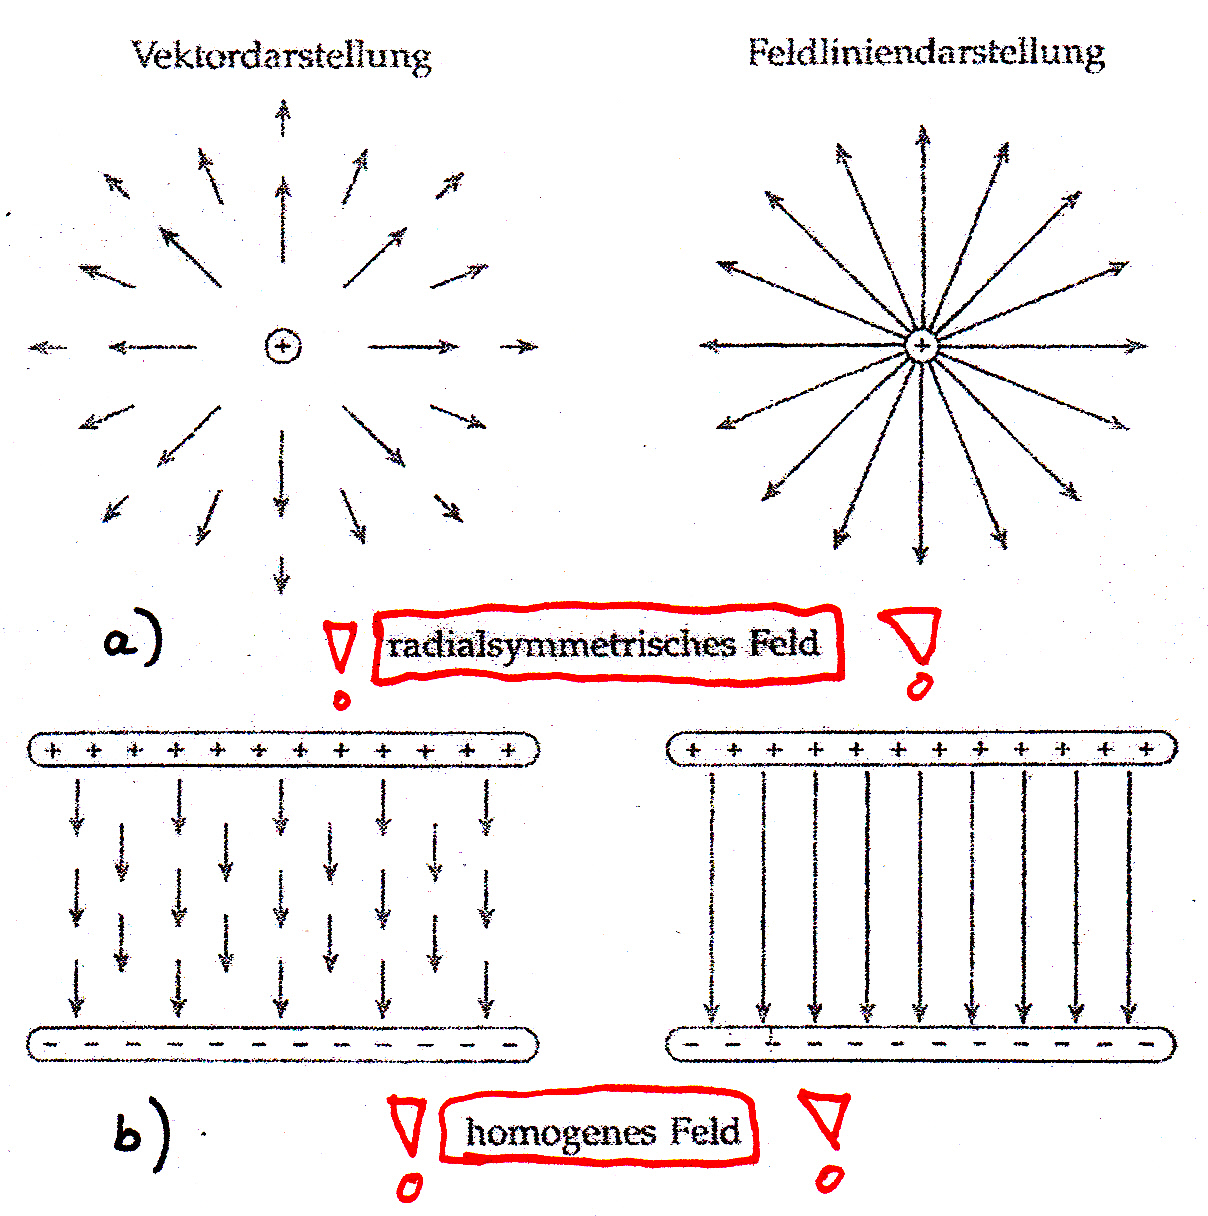
\includegraphics[scale=0.8]{hom_rad_feld}

\vspace{10mm}

\subsection{Darstellung des elektrischen Feldes durch Feldlinien - Aussagen des Feldlinienbildes}
1. An jedem Punkt erfährt eine Probeladung "q" eine Kraft tangential zu den Feldlinien. \\
2. Die Pfeile geben die Richtung der Feldkraft auf eine positive Probeladung an. \\
3. Das Feld ist an Stellen mit größerer Feldliniendichte stärker. \\
4. Feldlinien kreuzen sich nie. \\
5. Die Feldlinien stehen auf einem elektrischen Leiter immer senkrecht.
\vspace{2mm} \\
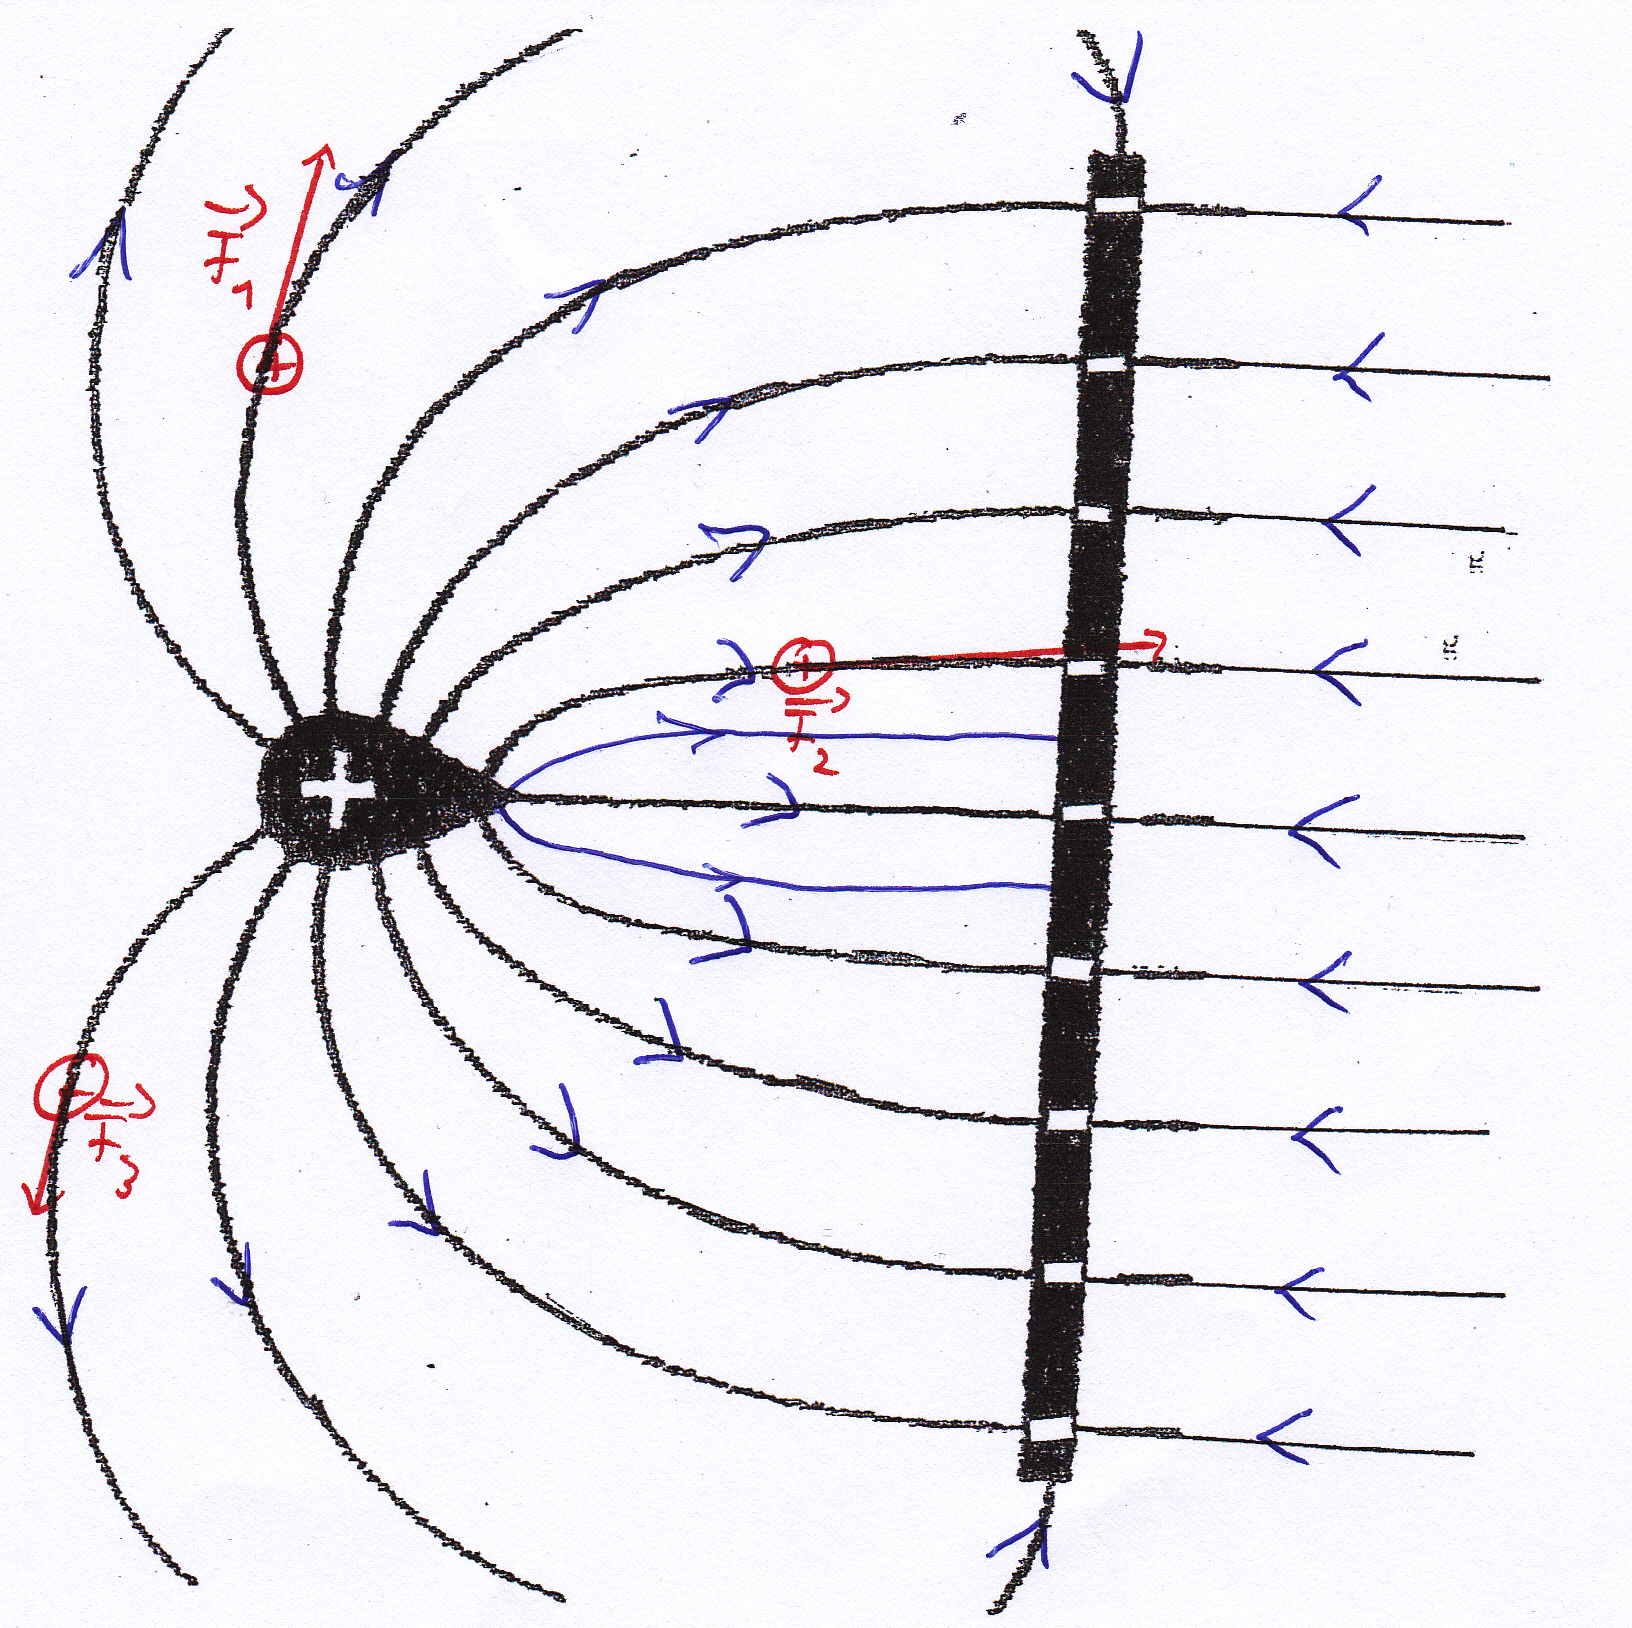
\includegraphics[scale=0.5]{feldlinien_leiter}

\vspace{2mm}
\underline{Merke:}

In der Elektrostatik gilt: \\
1. Feldlinien verlaufen nicht im geschlossenen Kreis, sondern sie beginnen bei positiven Ladungen und enden bei negativen. Wenn eine solche kreisförmige Feldlinie existieren würde, würde sich eine Ladung entlang dieser bewegen und dabei ständig Bewegungsenergie gewinnen ($ \lightning $ Energieerhaltungssatz) \\
2. Feldkräfte können in Leitern Ladungen verschieben. Im Inneren eines Leiters entsteht ein feldfreier Raum. \underline{(Bild faradayscher Käfig)} \\
3. In elektrostatischen Situationen gilt: Das elektrische Feld in einer leitenden Substanz ist überall 0. Die Ladung sitzt auf der Oberfläche der Substanz. \underline{(Bild von Leiter mit Ladung auf Oberfläche)} \\
4. Im Inneren eines Stromführenden Leiters (!Kein elektrostatischer Fall!) besteht ein Feld, das die Ladungen bewegt. 

\vspace{10mm}

\subsection{Vergleich zwischen elektrischem Feld und Gravitationsfeld}
\begin{tabular}{|l|l|l|}
	
	\hline & Gravitationsfeld & Elektrisches Feld\\
	\hline Feld: & Raumbereich, in dem Körper die &   Raumbereich, in dem Ladungen\\
	& Gravitationskräfte $ \vec{F}_{G} $ erfahren.& elektrische Kräfte $ \vec{F}_{el} $ erfahren. \\
	\hline Probekörper: & Probemasse m & Probleladung q \\
	\hline Felderzeugender & Körper mit Masse & Geladene Körper \\
	Körper: & (z.B. Erde) & (Felderzeugende Ladung Q) \\
	\hline Feldlinie: & Gedachte Linie, auf der sich eine & Gedachte Linie, auf der sich eine \\
	& Probemasse bewegt, wenn sie nur & positive Probeladung bewegt, wenn \\
	& der auf sie wirkenden $ F_{G} $ folgt. & sie nur der auf sie wirkenden $ F_{el} $ \\
	& Ihre Tangenten weisen an jeder & folgt. Ihre Tangenten  weisen an \\
	& Stelle der Feldlinie in Richtung & jeder Stelle der Feldlinie in Richtung \\
	& Gravitationskraft $ F_{G} $ & der elektrischen Kraft $ F_{el} $ \\
	\hline Eigenschaften von & 1. Zeigen in Richtung der Kraft & 1. Zeigen in Richtung der Kraft auf \\
	Feldlinien & auf eine Probemasse & eine positive Probeladung \\
	& 2. Zeigen stets zur felderzeugenden & 2. Sie verlaufen von positiver zu \\
	& Masse & negativer Ladung \\
	& 3. Kreuzen sich nie & 3. Kreuzen sich nie \\
	& & 4. Ein elektrischer Dipol stellt sich \\
	& & tangential zur Feldlinie ein. \\
	& & Seine positive Ladung zeigt in \\
	& & Richtung der Feldlinie \\
	\hline Kraft auf: m / q & $ \vec{F}_{G} = m \ast \vec{g} $ & $ \vec{F}_{el} = q \ast \vec{E} $ \\
	\hline Feldstärke & Gravit.-const. $ \vec{g} $ &  Elektr. Feldstärke $ \vec{E} $ \\
	\hline Energie: & $W_{pot} = m \ast g \ast h $ & $ W_{el} = q \ast \vec{E} \ast s = F_{el} \ast s  = q \ast U $ \\
	\hline Potential & $ \varphi_{G} = \dfrac{W_{pot}}{m} = g \ast h $ & $ \varphi_{el} = \dfrac{W_{el}}{q} = E \ast s $ \\
	\hline Potentialdifferenz & $ \varphi_{2} - \varphi_{1} = g \ast \Delta h  $ & $ U = \varphi_{2} - \varphi_{1} = E \ast \Delta s $ \\ \hline
	
\end{tabular}

\subsection{Die Flächenladungsdichte Sigma}
Der Quotient $ \sigma = \dfrac{Q}{A} $ heißt \underline{Flächenladungsdichte}. Die Einheit ist $ [\sigma] = \dfrac{1C}{1 m^{2}} $. \vspace{1mm} Die Feldstärke E eines homogenen Feldes ist der Flächenladungsdichte $ \sigma $ der sie erzeugenden Ladung proportional. \\
In Luft gilt: $ \sigma = \epsilon_{0} \ast \epsilon_{r} \ast E $

\vspace{10mm}

\subsection{Energie, elektrisches Potential und Spannung}
\subsubsection{Energieumwandlung im elektrischen Feld}
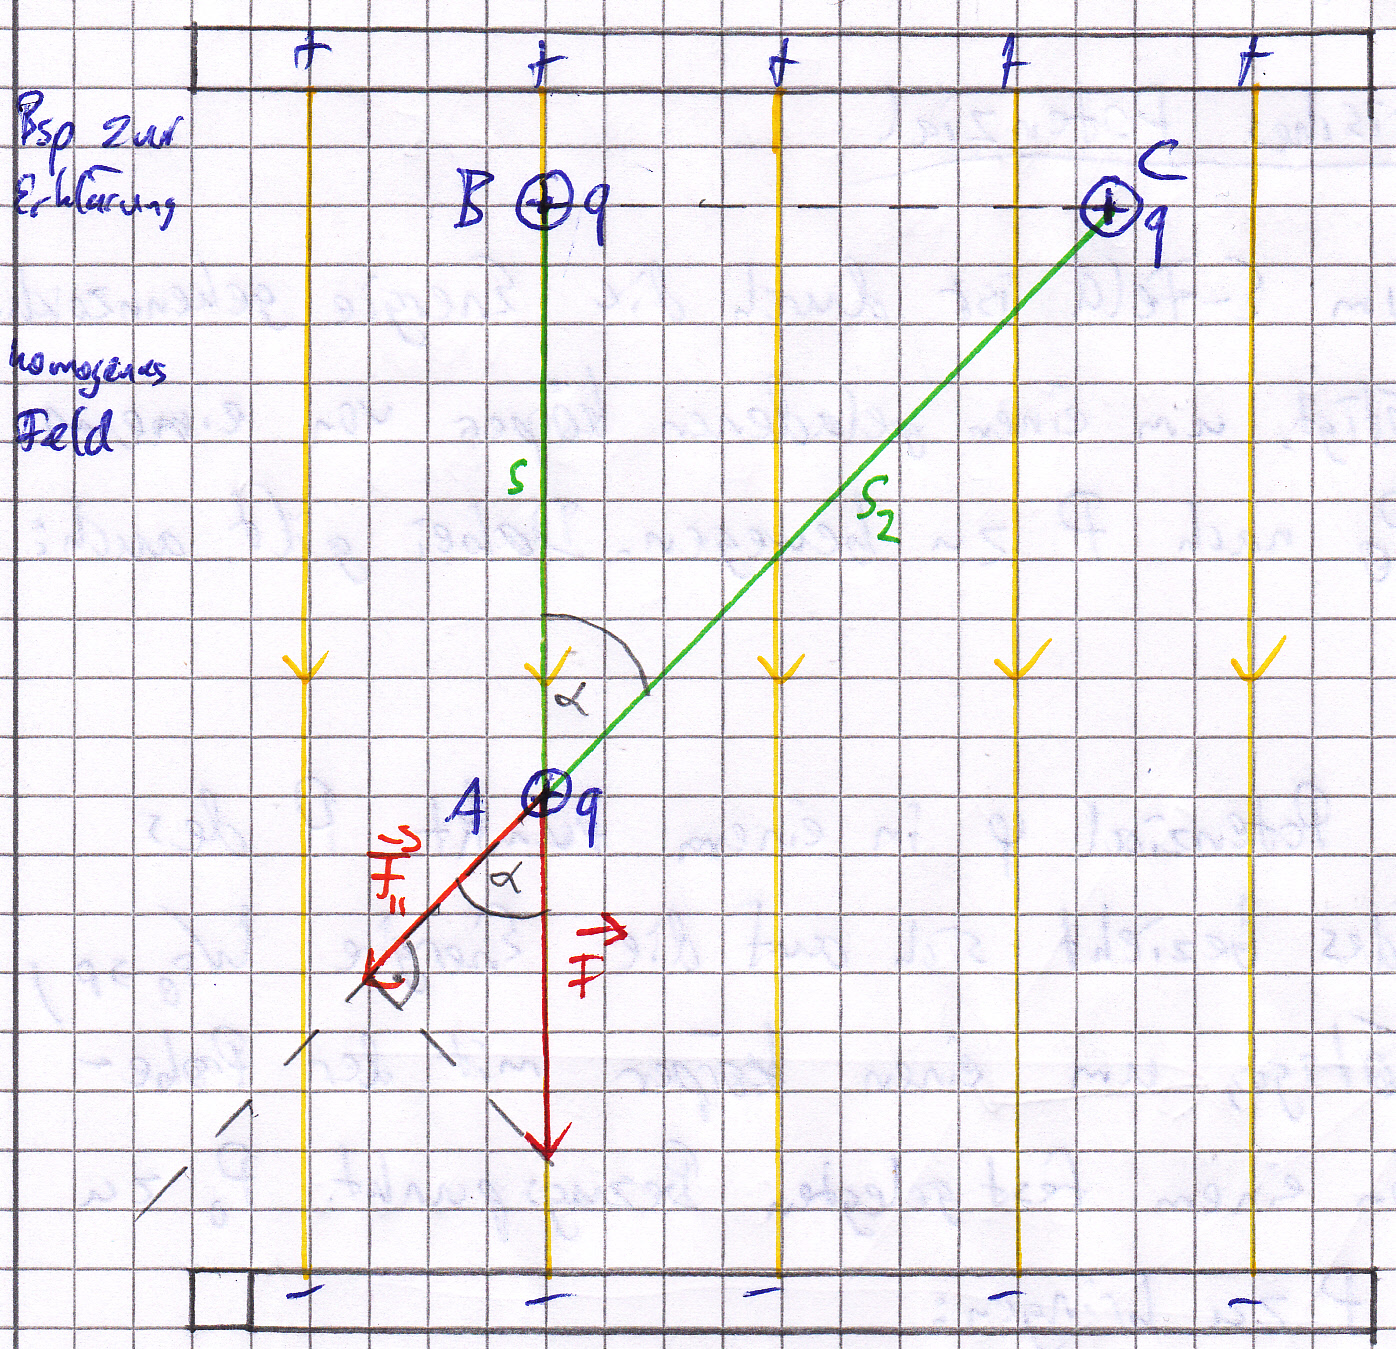
\includegraphics[scale=0.7]{I9_energieumwandlung} \\
Maßstab: 1N $\hat{=}$ 3cm

\vspace{5mm}
$ \vec{F}_{II} = \vec{F} \ast cos(\alpha) $ \hspace{5mm} $ s_{2} = \dfrac{s}{cos(\alpha)} $

\vspace{2mm}
$ W_{A \rightarrow B} = F \ast s $ (In diesem Beispiel: 0,05 J)

\vspace{2mm}
$ W_{A \rightarrow C} = F_{II} \ast s_{2} $ (In diesem Beispiel: 0,05 J)

\vspace{2mm}
$ \Rightarrow W = F \ast s $	

\vspace{2mm}
\underline{Merke:} \\
Verschiebt man einen geladenen Körper im E-Feld entgegen der Kraft, so wird ihm Energie zugeführt. Sie heißt - analog zum Fall des angehobenen Körpers im Gravitationsfeld - \underline{potentielle Energie}. Die Energieänderung bei der Verschiebung einer Ladung ist nur vom \underline{Anfangs- und Endpunkt} abhängig, nicht vom gewählten Weg. Deshalb kann man bei der Berechnung von $W_{pot}$ den Weg in Abschnitte parallel und senkrecht zur Feldlinienrichtung zerlegen, wobei dann nur der parallele Abschnitt einen Beitrag zur Energieänderung liefert. \\
Im \underline{homogenen Feld} ergibt sich: $ W = F \ast s = q \ast E \ast s $ 

\subsubsection{Elektrisches Potential}
Jeder Punkt im E-Feld ist durch die Energie gekennzeichnet, die man benötigt, um einen geladenen Körper von einem Bezugspunkt $P_{0}$ nach P zu bewegen. Dabei gilt auch:
\vspace{2mm} \\
$ W_{P_{0} \rightarrow P} \sim q $
\vspace{2mm} \\
Das elektrische Potential $\varphi$ in einem Punkt P des elektrischen Feldes bezieht sich auf die Energie $W_{P_{0} \rightarrow P}$, die man benötigt, um einen Körper mit der Probeladung q von einem festgelegten Bezugspunkt $P_{0}$ zu diesem Punkt P zu bringen:
\vspace{2mm} \\
$ \varphi_{P} = \dfrac{W_{P_{0} \rightarrow P}}{q} $ \hspace{5mm} $ [\varphi] = \dfrac{J}{C} = V $
\vspace{2mm} \\
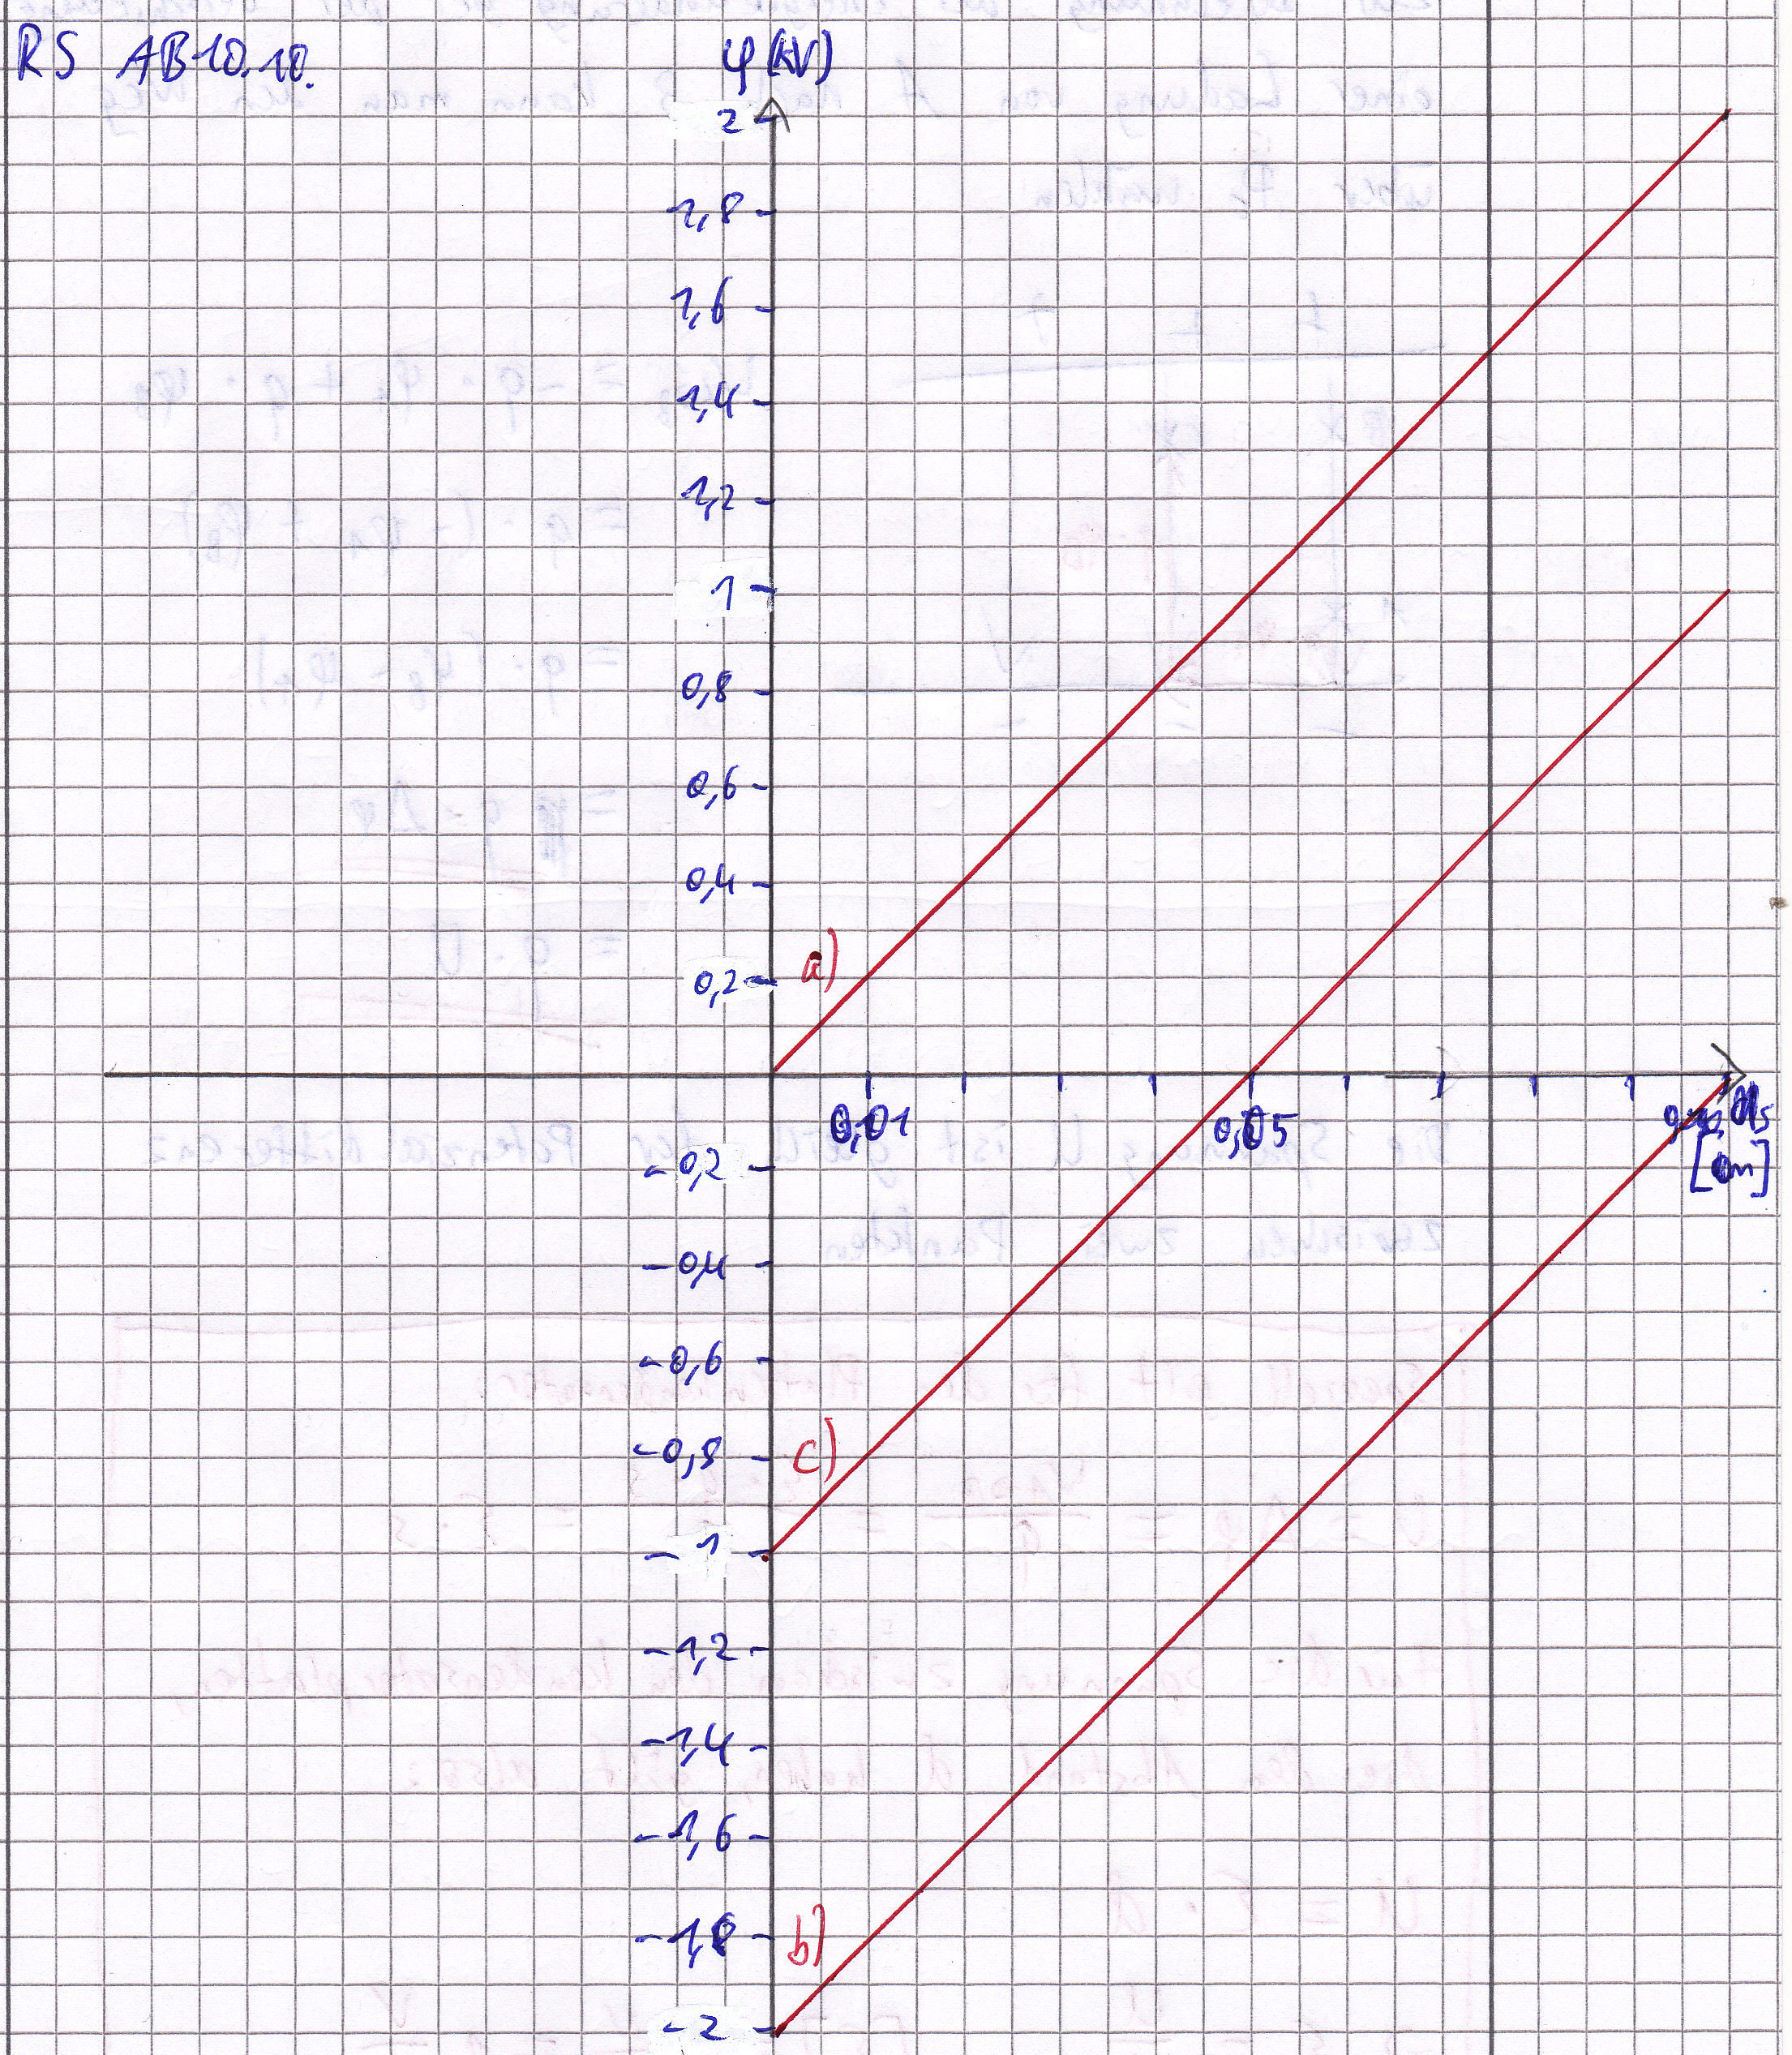
\includegraphics[scale=0.7]{I9_potential}
\vspace{2mm} \\
$\varphi_{(x)} = E \ast x + \varphi_{0}$ 

\vspace{2mm}
Bezugspunkte auf: \\
a) negativ geladener Platte \\
b) positiv geladener Platte \\
c) genau in der Mitte zwischen beiden Platten \\

\newpage

\subsubsection{Elektrische Spannung U}
Zur Berechnung der Energieänderung bei der Verschiebung einer Ladung von A nach B kann man den Weg über $P_{0}$ wählen. 

\vspace{2mm}
$ W_{A \rightarrow B} = -q \ast \varphi_{A} + q \ast \varphi_{B} $ \\
\hspace{11.5mm} $ = q \ast (- \varphi_{A} + \varphi_{B}) $ \\
\hspace{11.5mm} $ = q \ast \Delta \varphi $ \\
\hspace{11.5mm} $ = q \ast U  $ 
\vspace{2mm} \\
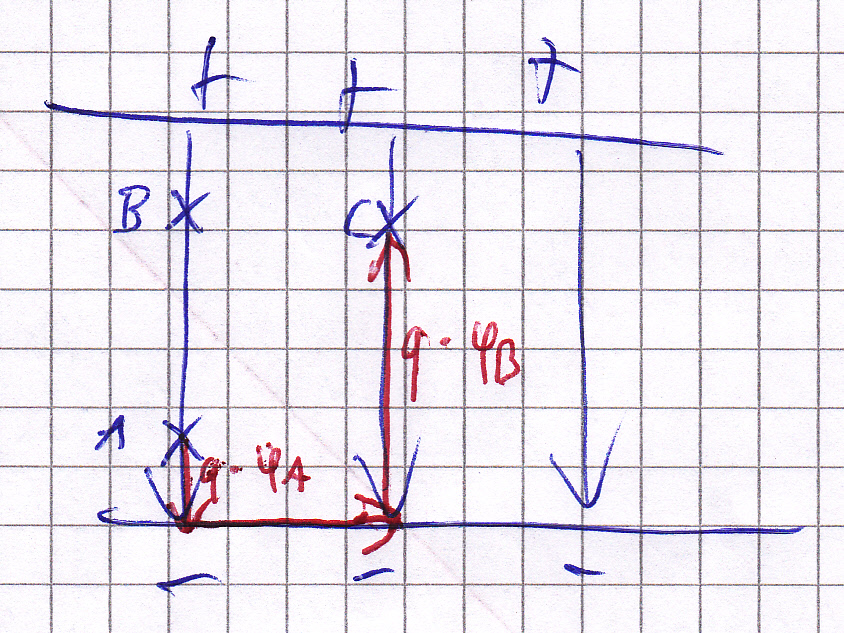
\includegraphics[scale=0.8]{I9_spannung}
\vspace{2mm} \\
Die Spannung U ist gleich der Potentialdifferenz zwischen zwei Punkten.

\vspace{5mm}
\underline{Speziell gilt für den Plattenkondensator:} \\
\vspace{2mm}
$ U = \Delta  \varphi = \dfrac{W_{A \rightarrow B}}{q} = \dfrac{E \ast q \ast s}{q} = E \ast s $

\vspace{2mm}
Für die Spannung zwischen den Kondensatorplatten, die den Abstand d haben, gilt also: \\
\vspace{2mm}
$ U = E \ast d $ \hspace{10mm} $ [E] = \dfrac{N}{C} = \dfrac{V}{m} $
\newpage
\subsubsection{Äquipotentiallinien}
Auf einer Fläche senkrecht zu den Feldlinien herrscht überall das gleiche Potential, da bei einer Verschiebung senkrecht zu den Feldlinien keine Energieänderung stattfindet. $\Rightarrow$ Äquipotentiallinien (unten in blau) \\
\vspace{3mm}
Je dichter die Äquipotentiallinien, desto größer die Energieänderung bei der Bewegung senkrecht dazu \\ $\Rightarrow$ desto größer ist die Feldstärke
\vspace{2mm}

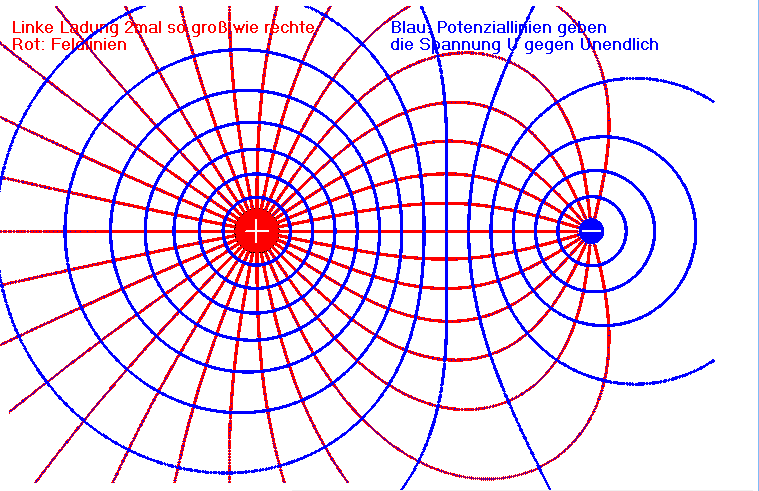
\includegraphics[scale=0.4]{I9_aequipotentiallinien}
\vspace{10mm}

\subsection{Geladene Teilchen im Längsfeld}
$ W_{A \rightarrow B} = q \ast U = q \ast \Delta \varphi $

\vspace{2mm}
Beim Durchfliegen der Beschleunigungsspannung U gewinnt das geladene Teilchen die Energie $ W = q \ast U $, falls die Spannung das Teilchen beschleunigt, andernfalls verliert dieses Energie (Siehe Buch S.20 B2).
\vspace{2mm} \\
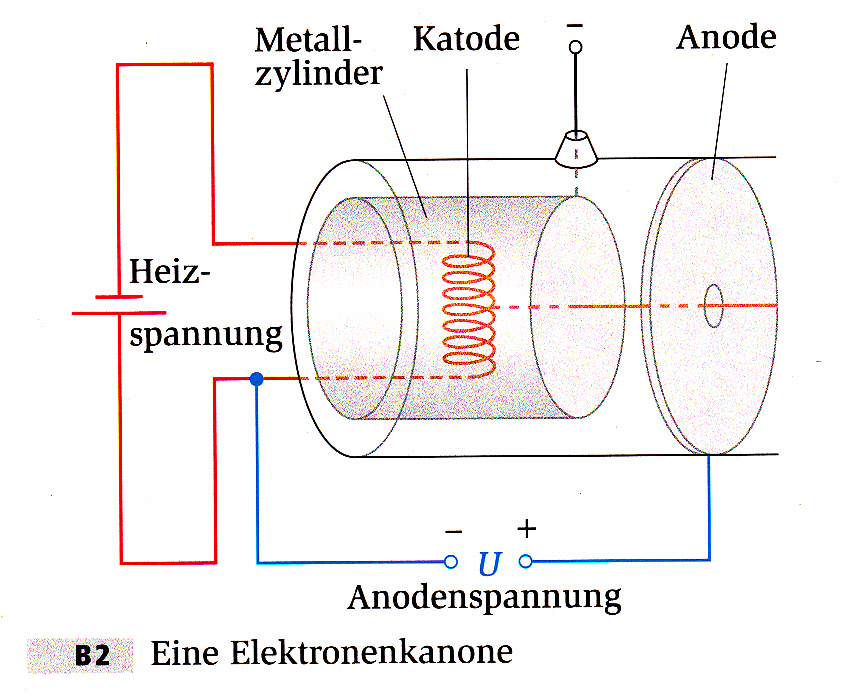
\includegraphics{I10_wehnelt}
\vspace{2mm} \\
Wird ein Elektron mit 250V beschleunigt, so hat dieses danach die Energiemenge $ W = q \ast U = e \ast U = e \ast 250V = 250 eV $ dazugewonnen.


\subsection{Kondensator-Kapazität}
\subsubsection{Ladung}
Wie viel Ladung fasst ein Kondensator bei vorgegebener angelegter Spannung U? (Bsp.: Plattenkondensator)
\vspace{2mm} \\
$ U = E \ast d $
\vspace{2mm} \\
Wir wissen bereits:
\vspace{2mm} \\
$ \sigma = \dfrac{Q}{A} $ und $ \sigma = \epsilon_{0} \ast E $
\vspace{2mm} \\
Daraus folgt:
\vspace{2mm} \\
\hspace{5mm}$ \dfrac{Q}{A} = \epsilon_{0} \ast E $\\ \vspace{4mm}$ \Rightarrow \dfrac{Q}{A} = \epsilon_{0} \ast \dfrac{U}{d} $\\ \vspace{4mm}$ \Rightarrow Q = \underbrace{\epsilon_{0} \ast \dfrac{A}{D}} \ast U $ \\
Konstante, genannt Kapazität C	

\vspace{5mm}
\underline{Allgemein gilt:}
Den Quotienten $\dfrac{Q}{U}$ nennt man Kapazität C. Die Ladung auf einem \\ \vspace{2mm}
Kondensator ist der angelegten Spannung proportional.

\vspace{5mm}
\underline{Merke:}
Anordnungen aus zwei Leitern, die durch einen Isolator getrennt sind, heißen Kondensatoren. Aufgrund ihrer Fähigkeit, Ladungen und Energie zu speichern, werden sie vielfältig eingesetzt. Die Kapazität C gibt an, wie viel Ladung der Kondensator bei einer bestimmten Spannung speichern kann:
\vspace{2mm} \\
$ C = \dfrac{Q}{U} $ \hspace{5mm} $ [C] = \dfrac{1C}{1V} = 1F $ (Farad; Nach Michael Faraday)
\vspace{5mm} \\
Symbol: 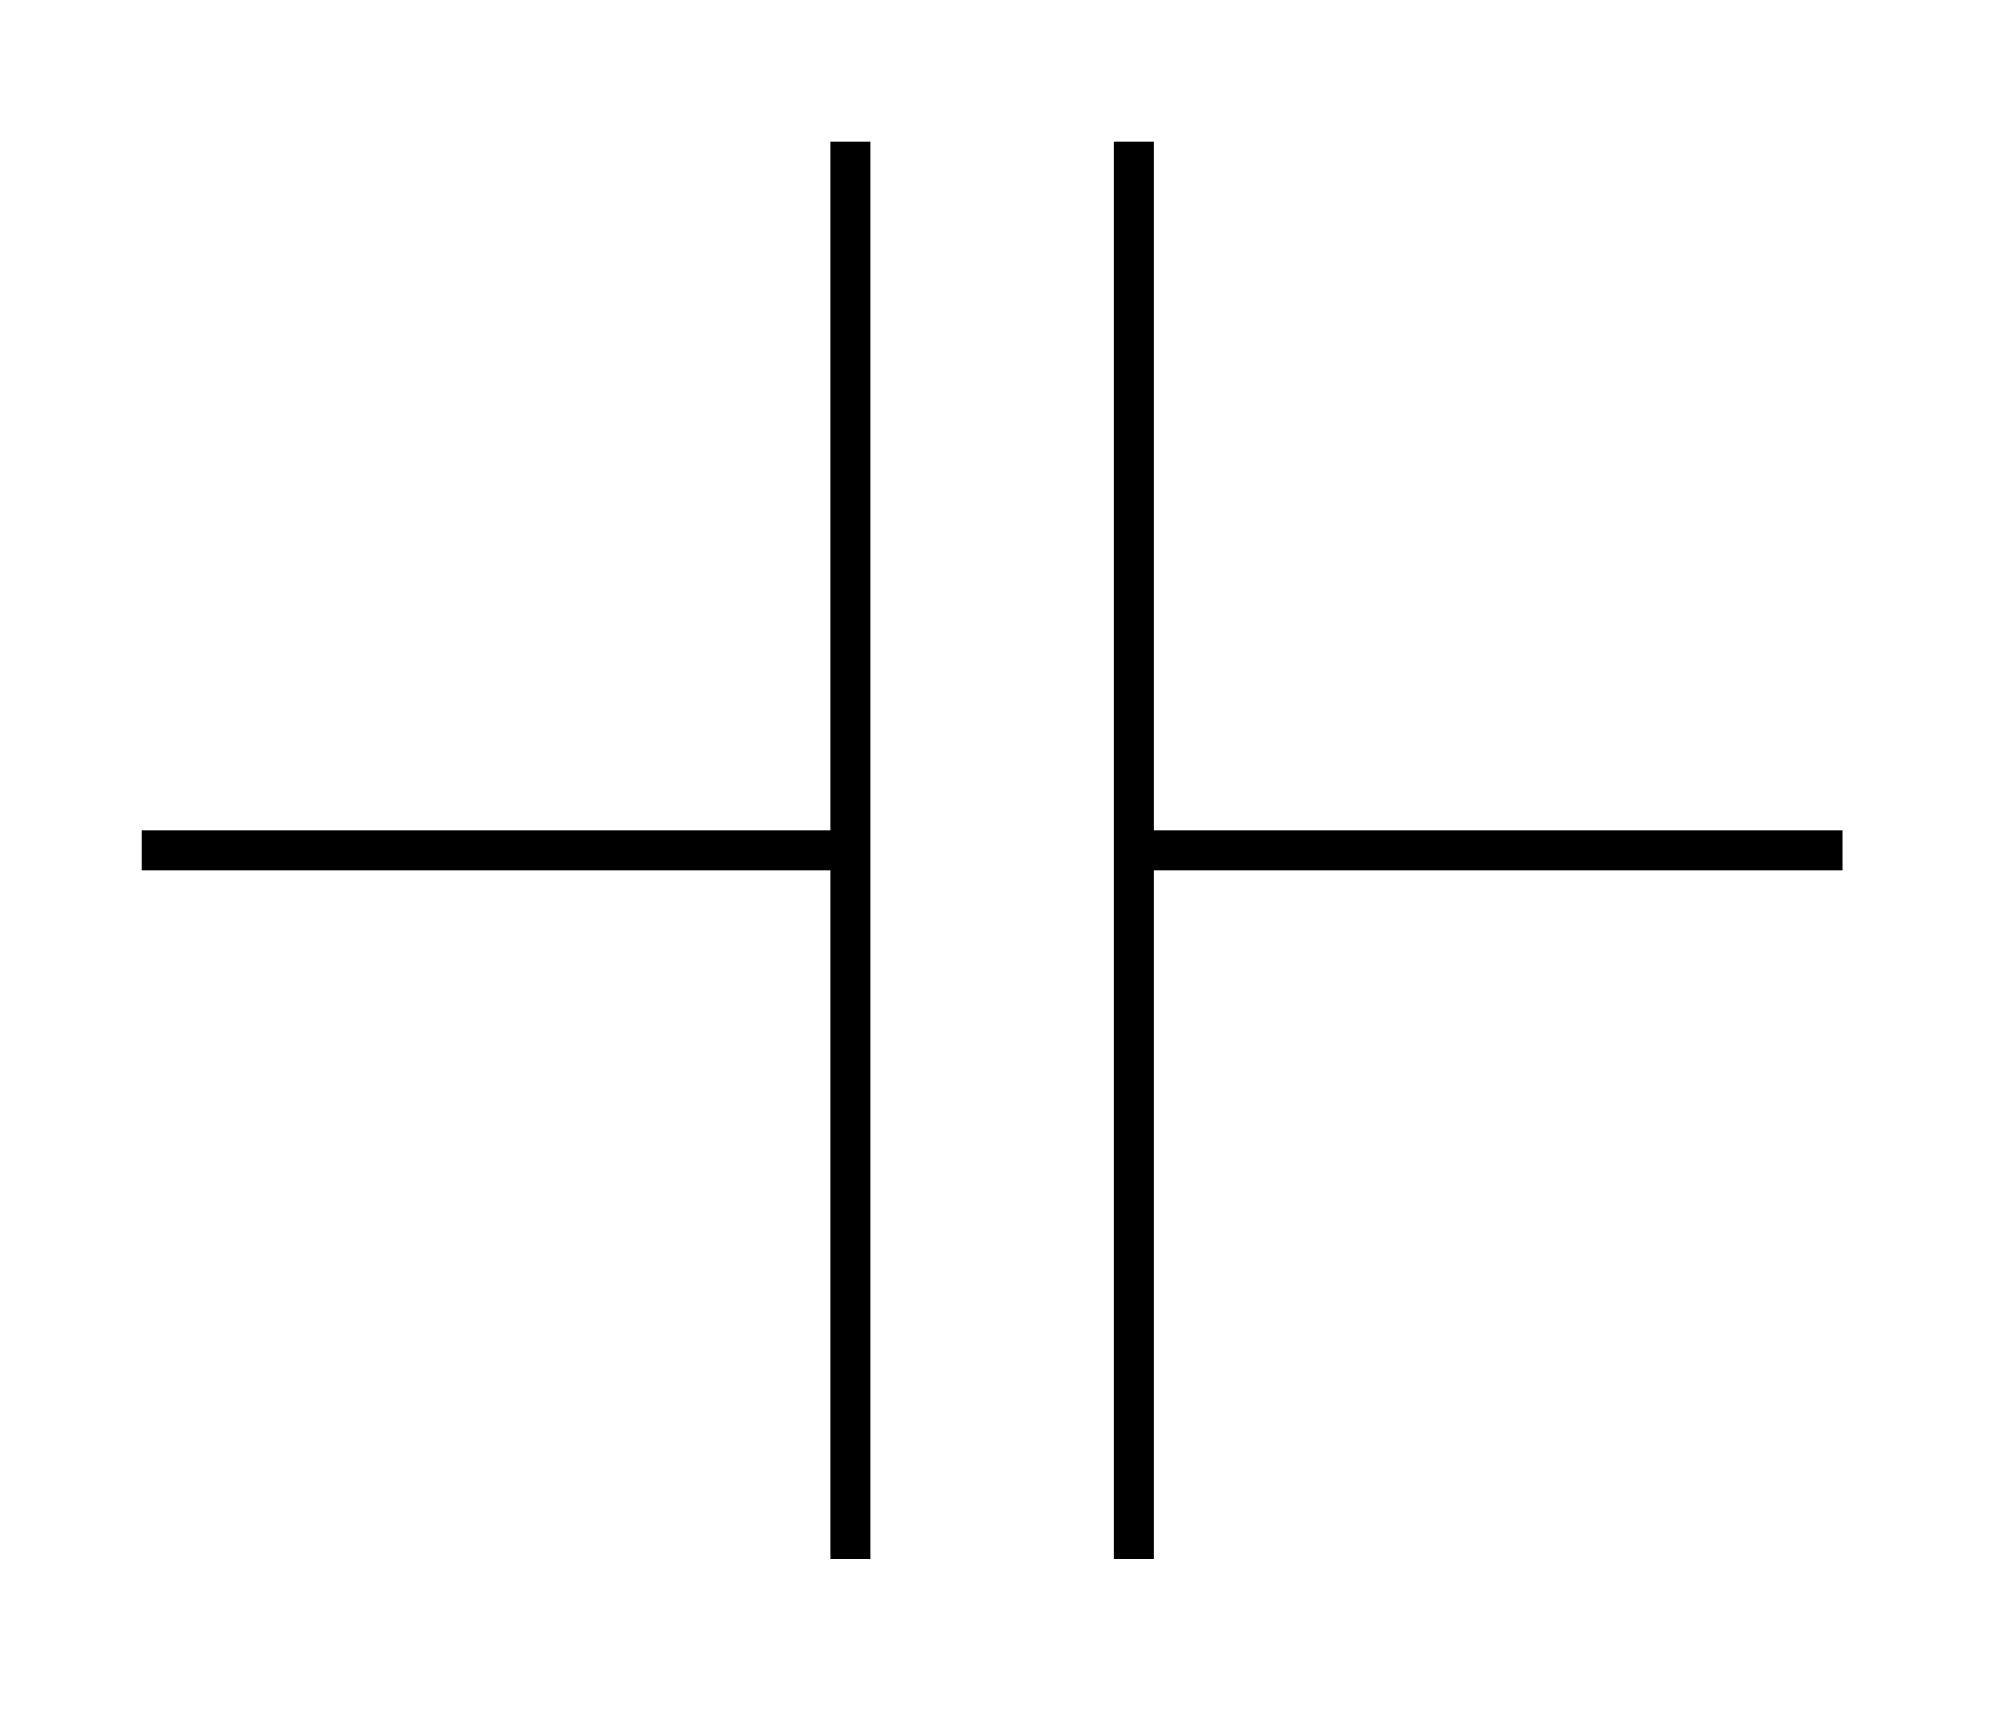
\includegraphics[scale=0.015]{capacitor}
\vspace{5mm} \\
Speziell: Die Kapazität eines \underline{Plattenkondensators im Vakuum} wird durch die Plattenfäche A und den Abstand D bestimmt. 
\vspace{2mm} \\
$ C = \epsilon_{0} \ast \dfrac{A}{d} $
\newpage
\subsection{Kondensator-Entladung und -Aufladung}
\underline{Schaltplan:}
\vspace{2mm} \\
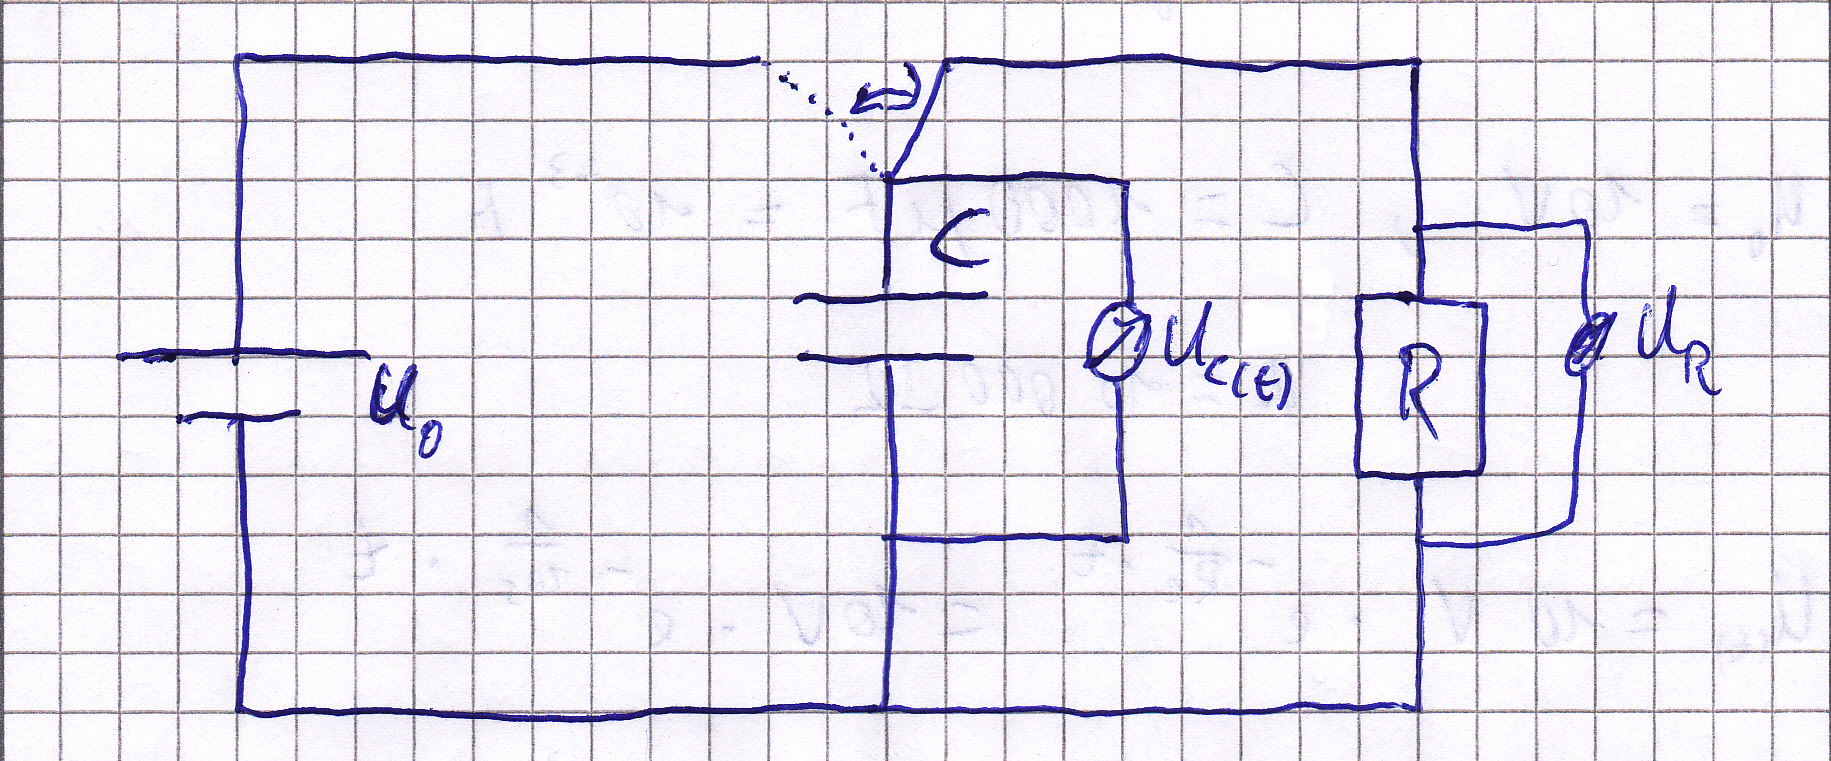
\includegraphics[scale=0.5]{I12_schaltplan}
\vspace{2mm}

$ U_{C(t)} = \dfrac{Q_{(t)}}{C} $
\vspace{2mm} \\
Bei uns: R = 10 k$\Omega$; C = 1000 $ \mu F $; $U_{0} = 10V$ \\
Beim Entladevorgang gilt: \\
\vspace{3mm}
$ U_{C(t)} = -R \ast I $ \hspace{40mm} (Maschenregel: $U_{C(t)} + U_{R} = 0$)
\vspace{5mm} \\
$ \dfrac{Q_{(t)}}{C} = -R \ast I $ \hspace{40mm} ( $\lim\limits_{\Delta t \rightarrow \infty}{\dfrac{\Delta Q}{\Delta t}} = \dot{Q}_{(t)}$ )
\vspace{5mm} \\
$ \dfrac{Q_{(t)}}{C} = -R \ast \dot{Q}_{(t)} $
\vspace{5mm} \\
$ \dot{Q}_{(t)} = \dfrac{Q_{(t)}}{\frac{C}{-R}} = \underbrace{\dfrac{-1}{C \ast R}} \ast Q_{(t)}$ \\
\hspace{24mm} Faktor
\vspace{5mm} \\
$ e^{x} = \dfrac{1}{0!}x^{0} + \dfrac{1}{1!}x^{1} + \dfrac{1}{2!}x^{2} + ... + \dfrac{1}{n!}x^{n}$ \hspace{2mm} $ \Rightarrow (e^{x})' = e^{x} $
\vspace{3mm} \\
\underline{Lösung:} $ Q_{(t)} = Q_{0} \ast e $ \hspace{15mm} $ \dot{Q}_{(t)} = Q_{0} \ast (-\dfrac{1}{C \ast R}) \ast e^{-\frac{1}{C \ast R} \ast t} $
\vspace{10mm} \\
$ U_{(t)} = \dfrac{Q_{(t)}}{C} = \underbrace{\dfrac{Q_{0}}{C}} \ast e^{-\frac{1}{C \ast R} \ast t} $ \\
\hspace{25.5mm} $U_{0}$
\vspace{5mm} \\
$ \dot{U}_{(t)} = - \dfrac{1}{C \ast R} \ast U_{(t)} $
\vspace{5mm} \\
$ 1F = \dfrac{1C}{1V} = \dfrac{1C}{1A \ast 1 \Omega} = \dfrac{1 As}{1A \ast 1 \Omega} = \dfrac{1s}{1 \Omega} $
\vspace{5mm} \\
$ F \ast \Omega = \dfrac{s}{\Omega} \ast \Omega = s $

\subsection{Mehrkapazität durch Isolatoren}
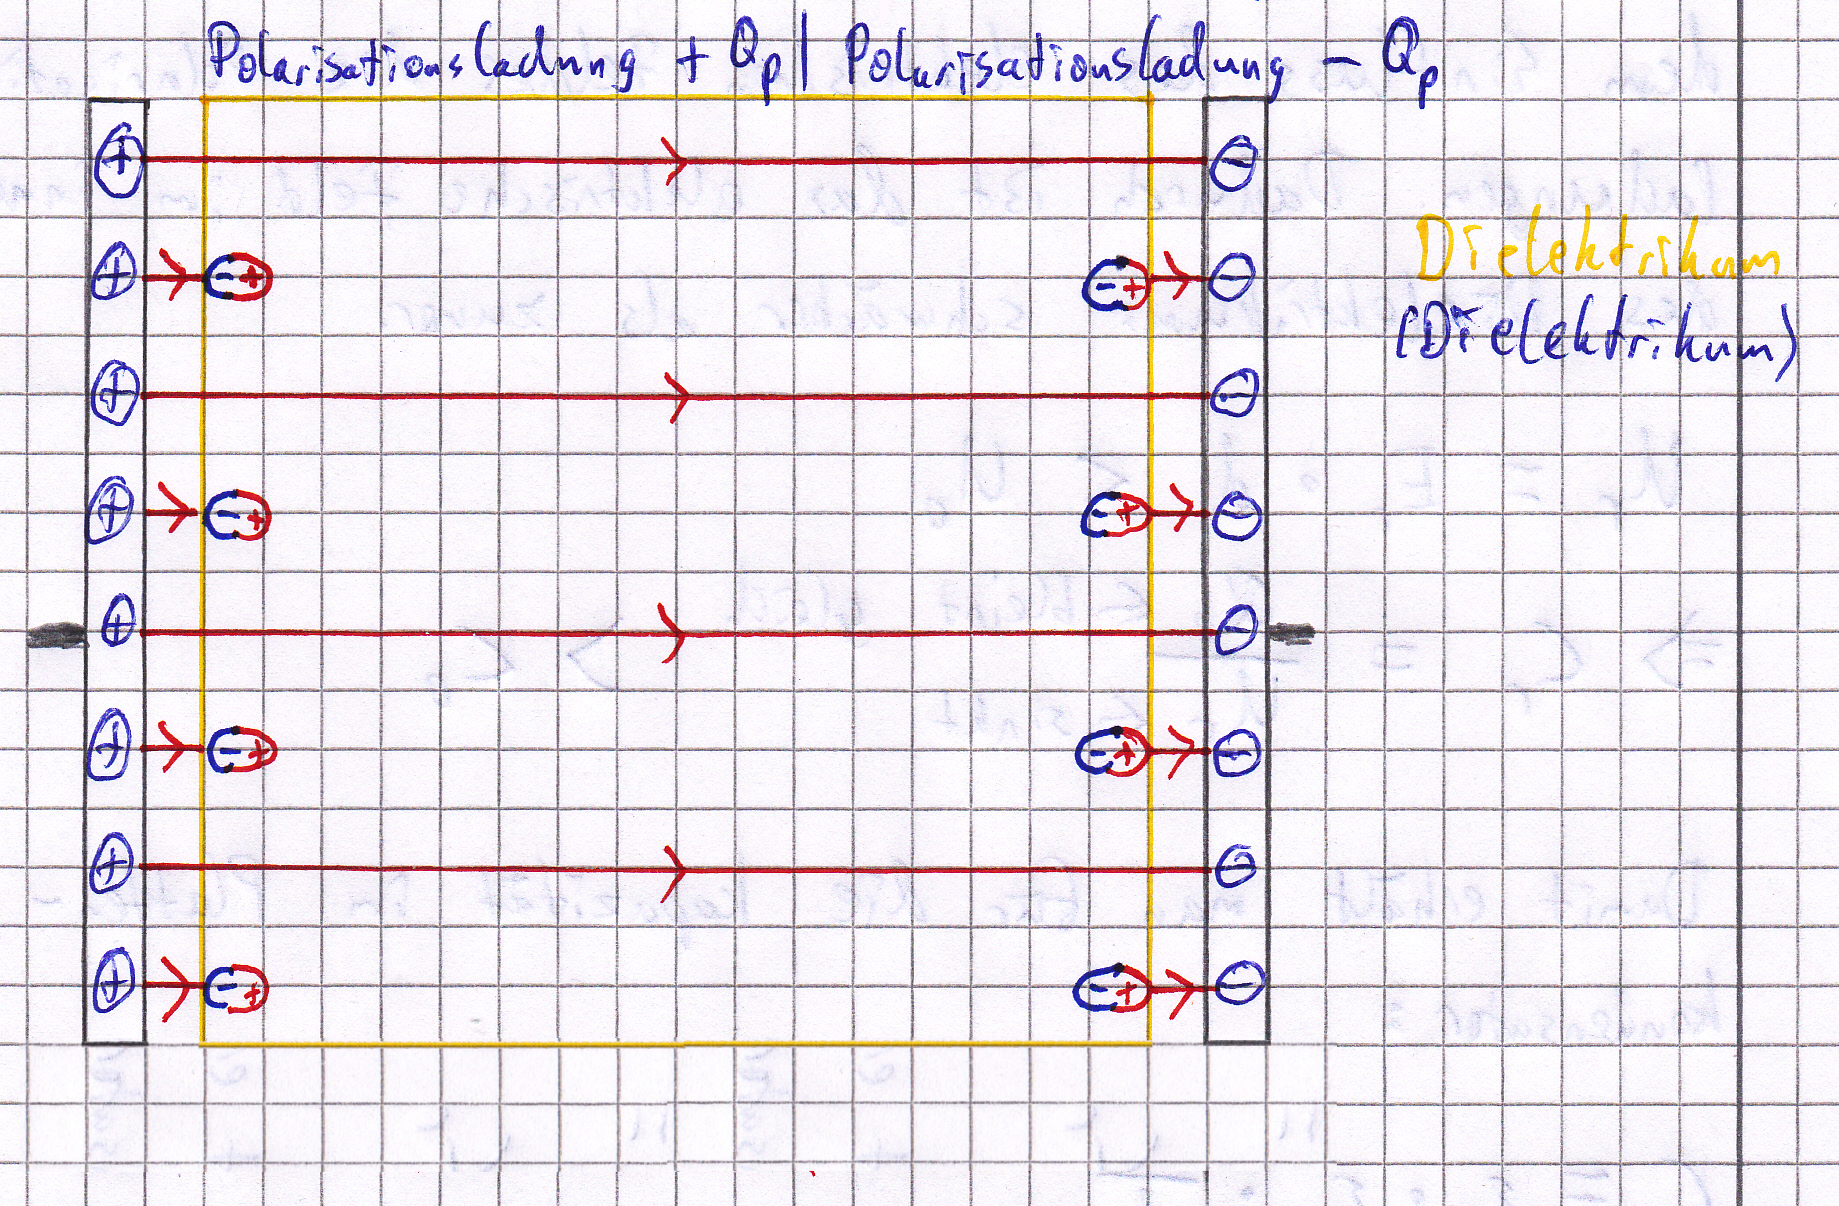
\includegraphics[scale=0.8]{I13_isolator} \\
\vspace{2mm}
$ E_{r} = \dfrac{E_{0}}{2} $ \hspace{20mm} (U = $ E \ast d $) 
\vspace{4mm} \\
$ \rightarrow U_{r} = \dfrac{U_{0}}{2} $
\vspace{4mm} \\
$ \rightarrow C_{r} = \dfrac{Q_{0}}{\frac{U_{0}}{2}} = 2 \ast C_{0} $
\vspace{6mm} \\
im Beispiel: $ \underbrace{\epsilon_{r}} = 2 $ \\
\hspace{12mm} Sprich: Epsilon r
\vspace{5mm} \\
\underline{Merke:} \\
In dem Isolator (Dielektrikum) verschieben sich unter dem Einfluss des elektrischen Feldes die Polarisationsladungen. Dadurch ist das elektrische Feld im inneren des Dielektrikums schwächer als zuvor. 
\vspace{5mm} \\
$ U_{r} = E_{r} \ast d < U_{0} $
\vspace{5mm} \\
$ \Rightarrow C_{r} = \dfrac{Q_{0} (\leftarrow bleibt)}{U_{r} (\leftarrow sinkt)} > C_{0} $
\vspace{3mm} \\
Damit erhält man für die Kapazität im Plattenkondensator: 
\vspace{2mm} \\
$ C = \epsilon_{0} \ast \underbrace{\epsilon_{r}} \ast \dfrac{A}{d} $ \\
\vspace{1mm}
\hspace{4mm} Dielektrizitätszahl

\subsection{Energie in elektrischen Feldern}
Wird der Kondensator aufgeladen, so steigt mit zunehmender Ladung Q auf den Kondensatorplatten auch die Spannung U. Um den Kondensator mit der zusätzlichen Ladung $\Delta Q$ weiter aufzuladen, ist die Energiemenge $\Delta W = \Delta Q \ast U_{(Q)} $ notwendig.
\vspace{2mm} \\
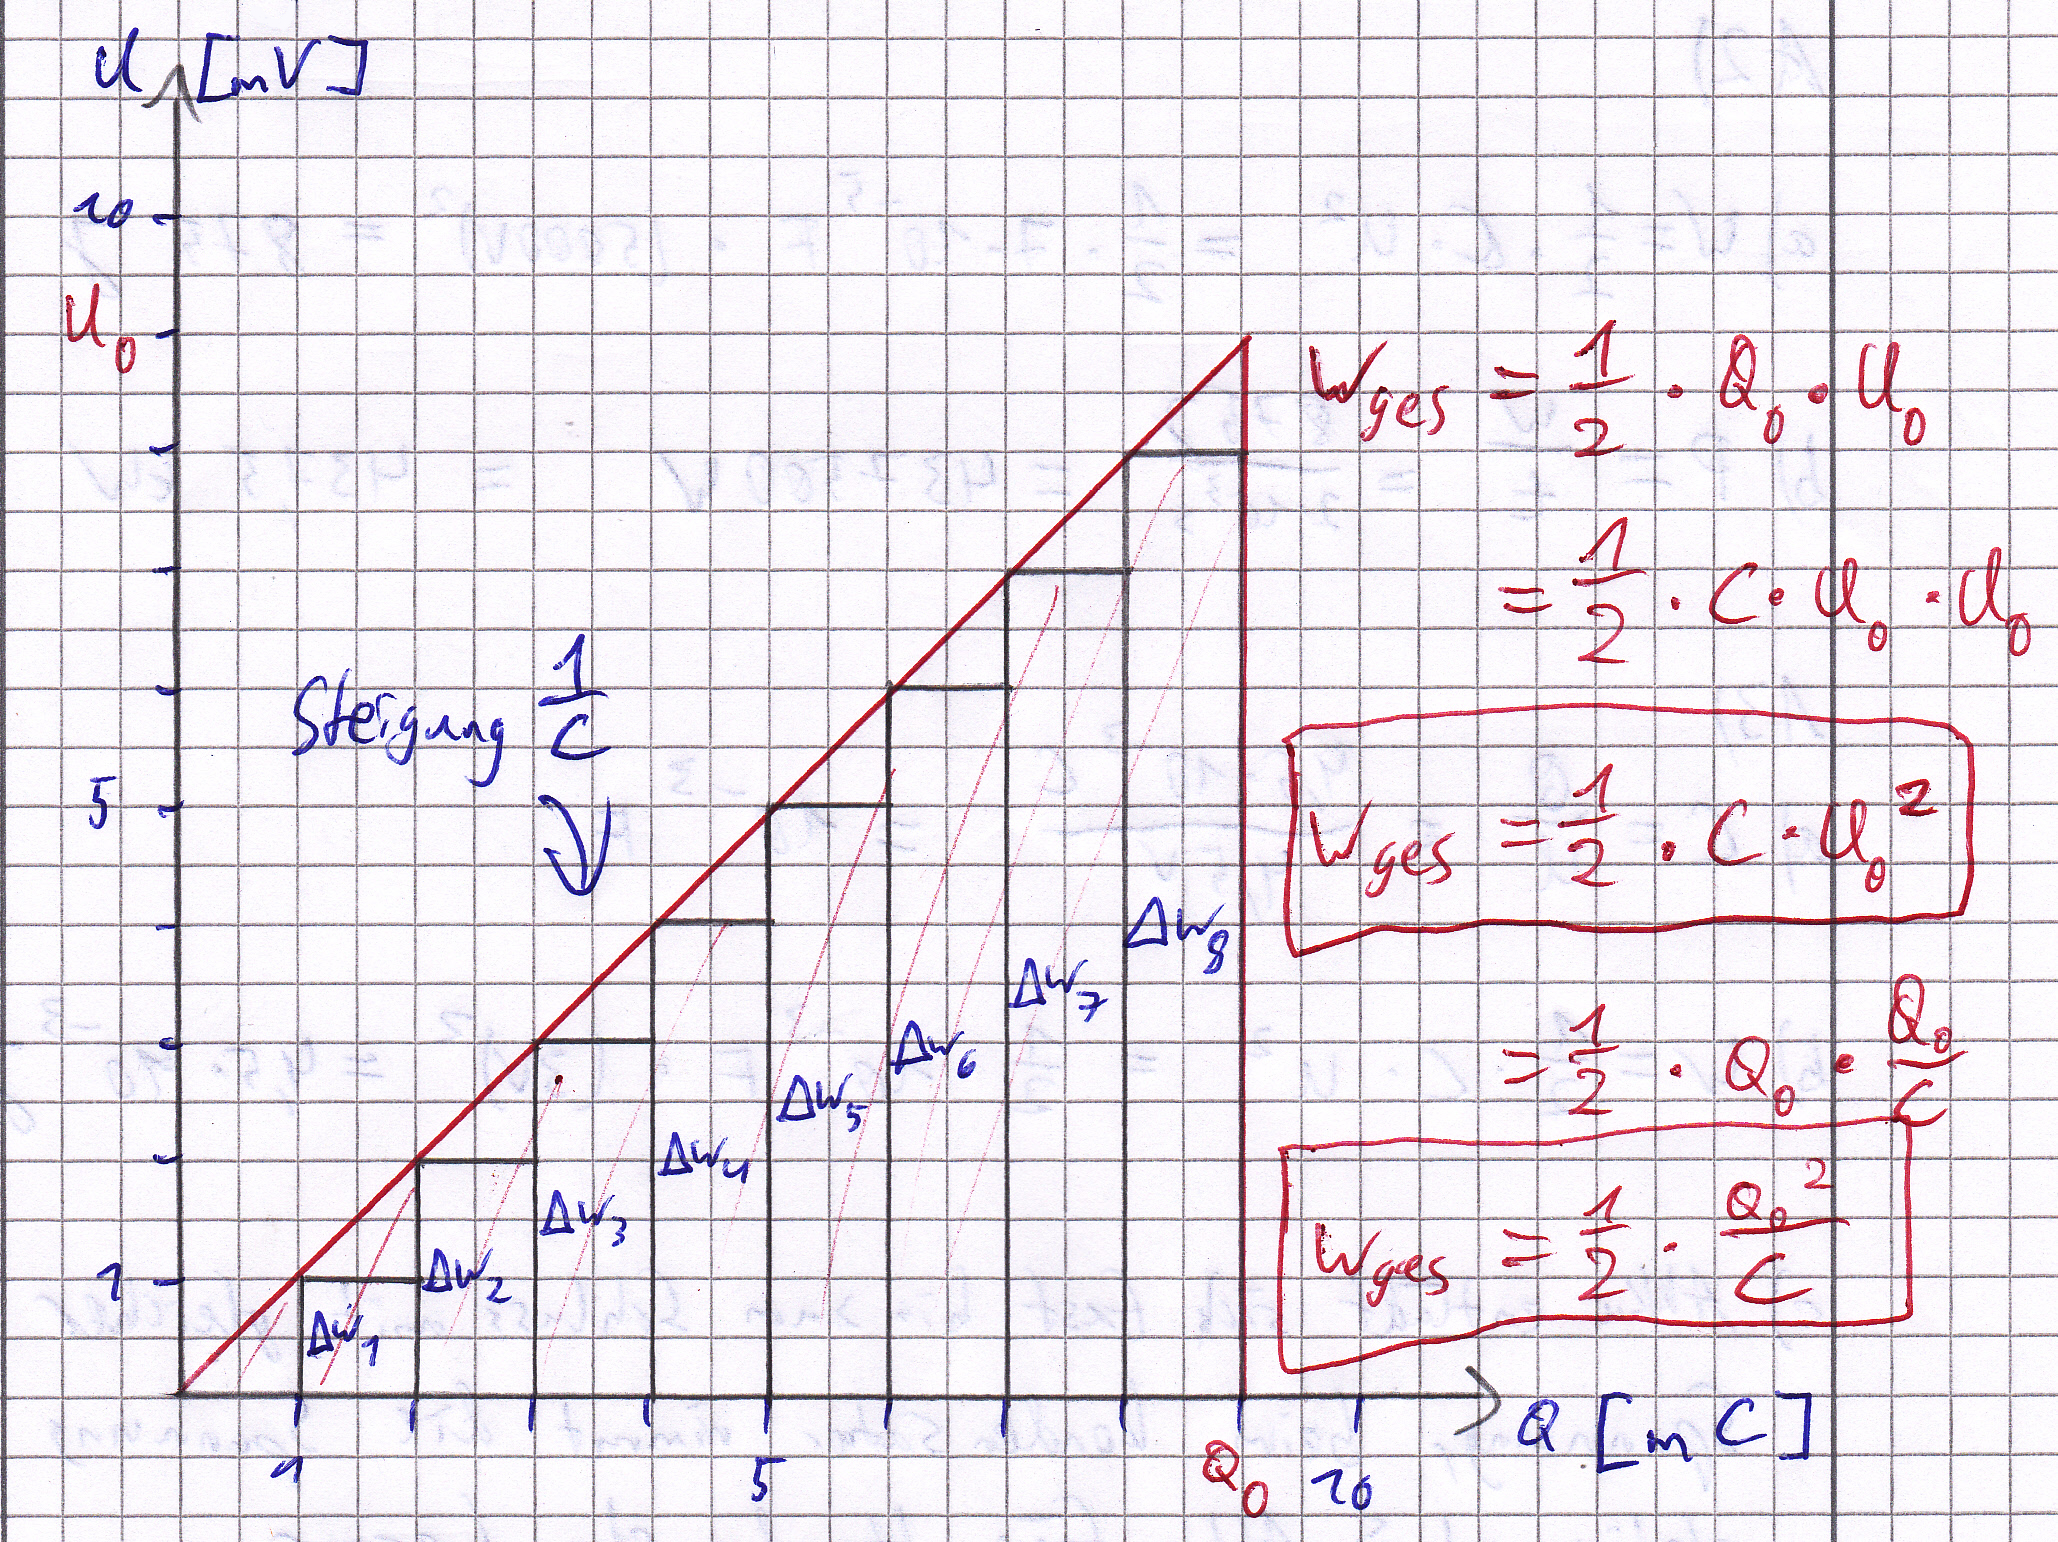
\includegraphics[scale=0.6]{I14_energie}
\vspace{2mm} \\
Die gesamte im Kondensator gespeicherte Energie ergibt sich aus dem Flächeninhalt unter dem Graphen im Q-U-Diagramm (Dabei ist $Q_{0}$ die Ladung, die der Kondensator am Ende trägt und $U_{0}$ die Spannung, auf die er aufgeladen wird).

\subsection{Parallel- und Reihenschaltung von Kondensatoren}
\subsubsection{Parallelschaltung}
$U_{ges} = U_{1} = U_{2}$
\vspace{2mm} \\
$Q_{ges} = Q_{1} + Q_{2}$
\vspace{2mm} \\
$C_{ges} = C_{1} + C_{2}$

\subsubsection{Reihenschaltung} 
$U_{ges} = U_{1} + U_{2}$
\vspace{2mm} \\
$Q_{ges} = Q_{1} = Q_{2}$
\vspace{3mm} \\
$\dfrac{C_{1}}{C_{2}} = \dfrac{U_{2}}{U_{1}}$
\vspace{3mm} \\
$\dfrac{1}{C_{ges}} = \dfrac{1}{C_{1}} + \dfrac{1}{C_{2}}$
	\section{Das Magnetfeld und Teilchen in Feldern}
\subsection{Eigenschaften von Magnetfeldlinien}
\begin{itemize}
	\item \glqq Starten\grqq\ am Nordpol und \glqq enden	\grqq\ am Südpol
	\item Je dichter die Linien, desto stärker ist das Magnetfeld
	\item Magnetfeldlinien haben keinen Anfang und kein Ende, sondern laufen durch den Magnet hindurch
	\item Magnetfeldlinien können durch einen Kompass oder Eisenspäne sichtbar gemacht werden
	\item Die Lorentzkraft wirkt senkrecht zu den Magnetfeldlinien und senkrecht zur Bewegungsrichtung der el. Ladung
	\item Der magnetische Südpol eines Probemagneten richtet sich entlang der Feldlinien zum Nordpol des erzeugten Feldes aus
	\item Magnetfeldlinien berühren sich nie
	\item Änderungen im Magnetfeld breiten sich mit Lichtgeschwindigkeit aus
	\item Feldrichtung ist die, in die eine Kompassnadel zeigen würde
\end{itemize}

\subsection{Magnetfeld von stromdurchflossenen Leitern}
\subsubsection{Magnetfeld eines stromdurchflossenen Leiters}
Der Leiter ist von magnetischen Feldlinien in Form von konzentrischen Kreisen umgeben. \\
\paragraph{Linke-Hand-Regel:} Zeigt der Daumen in Richtung der Elektronenbewegung, so zeigen die Finger der gekrümmten Hand die Richtung des Magnetfeldes an. 
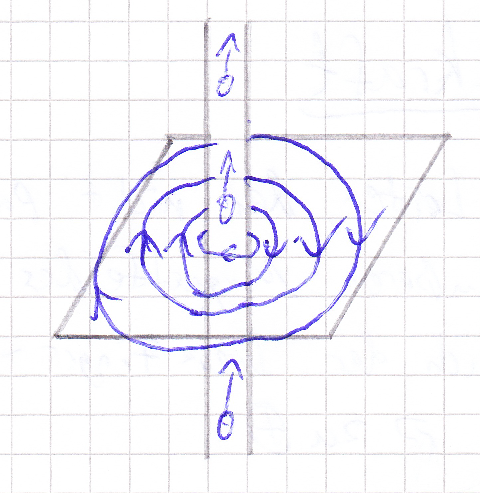
\includegraphics[scale=0.5]{221_magnetfeldlinien}

\subsubsection{Magnetfeld in einer stromdurchflossenen Leiterschleife}
Eine stromdurchflossene Leiterschleife erzeugt ein Magnetfeld wie ein kurzer, dicker Stabmagnet \\
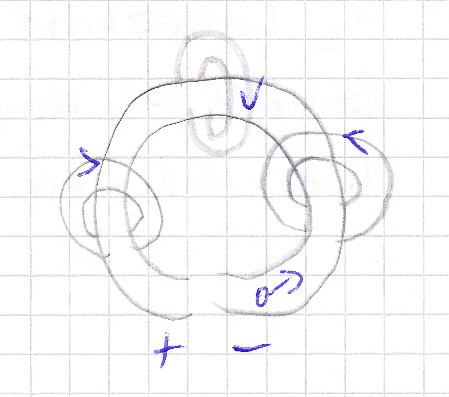
\includegraphics[scale=0.5]{222_magnetfeldlinien}

\subsubsection{Magnetfeld einer langen stromdurchflossenen Spule}
Im inneren ist das Feld homogen, innen laufen die Magnetfeldlinien von Süd nach Nord (wie in jedem Magneten) \\
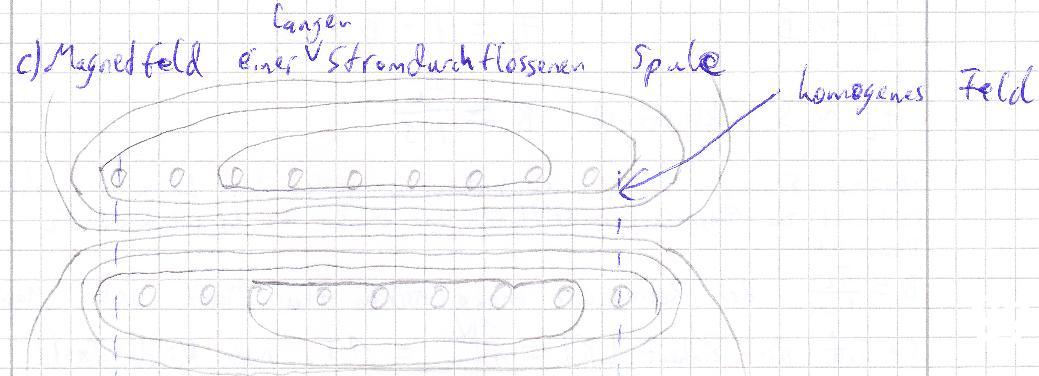
\includegraphics[scale=0.5]{223_magnetfeldlinien}
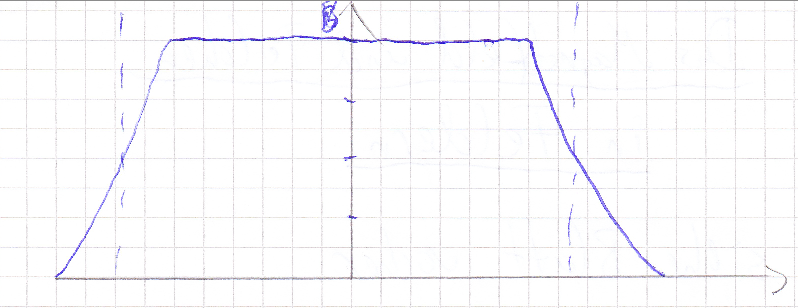
\includegraphics[scale=0.535]{223_homogenitaet}
\newpage

\subsection{Die Lorentzkraft}
Ein stromdurchflossener Leiter, der nicht parallel zu den Feldlinien eines äußeren Magnetfeldes steht, erfährt Lorentzkräfte nach der Drei-Finger-Regel. \\
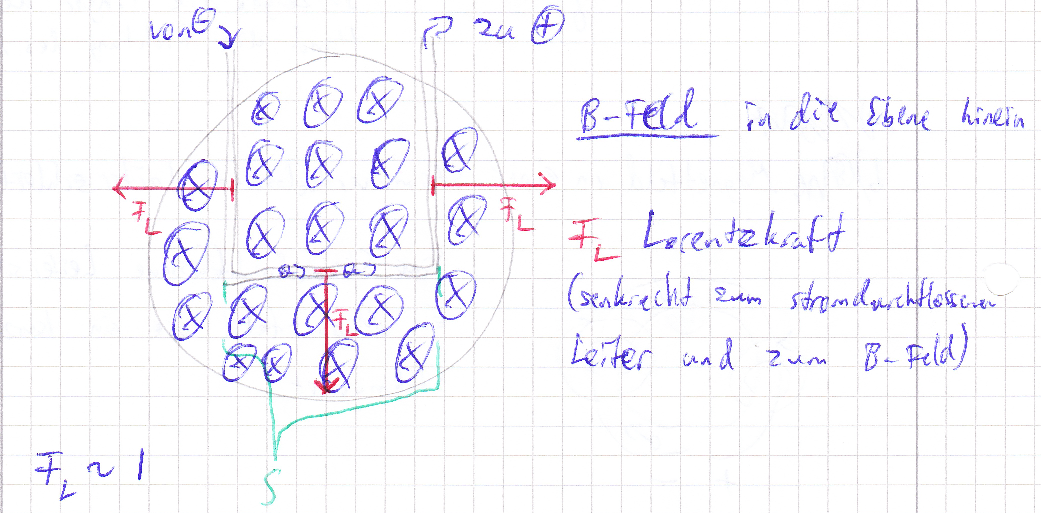
\includegraphics[scale=0.5]{23_Lorentzkraft} \\
$ F_L \sim I $ 
\vspace{1mm} \\
$ F_L \sim B $
\vspace{1mm} \\
$ F_L \sim s $
\vspace{1mm} \\
$ F_L = I \ast B \ast s $
\vspace{1mm} \\
$ B = \frac{F_L}{I \ast s} $

\paragraph{Definition:} Ein vom Strom I durchflossener Leiter der Länge s stehe senkrecht zu magnetischen Feldlinien und erfahre die Lorentzkraft $F_L$. Dann ist $B = \frac{F_L}{I \ast s}$ der Betrag der magnetischen Flussdichte des Magnetfeldes. Sie hat die Einheit $ [B] = \frac{1N}{1A \ast m} = 1T$ nach Nicola Tesla.

\subsection{Magnetische Kraft auf bewegte Ladungen}
Die eigentliche Ursache der Kraft auf einen stromdurchflossenen Leiter ist die Kraft, die im Magnetfeld auf bewegte Ladung wirkt, die sich nicht parallel zum Magnetfeld bewegt. Aus dem Leiterschaukelversuch erhält man:
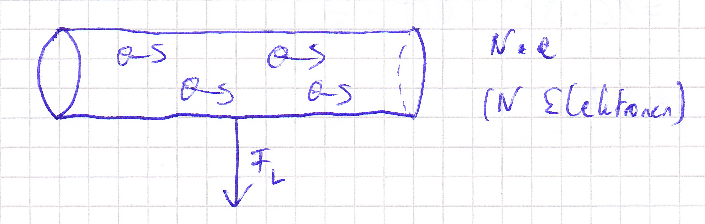
\includegraphics[scale=0.5]{24_leiterschaukel}
\vspace{3mm} \\
$F_L = I \ast B \ast s = \frac{Q}{t} \ast B \ast s = \frac{N \ast e}{t} \ast B \ast s = N \ast e \ast v \ast B$
\vspace{3mm} \\
$ \Rightarrow F_L $ auf ein einzelnes Elektron: $ F_L = e \ast v \ast B $

\newpage

\paragraph{Allgemein gilt:} $F_L = q \ast v \ast B $ \hspace{2mm} wenn \hspace{2mm} $ v \perp B $
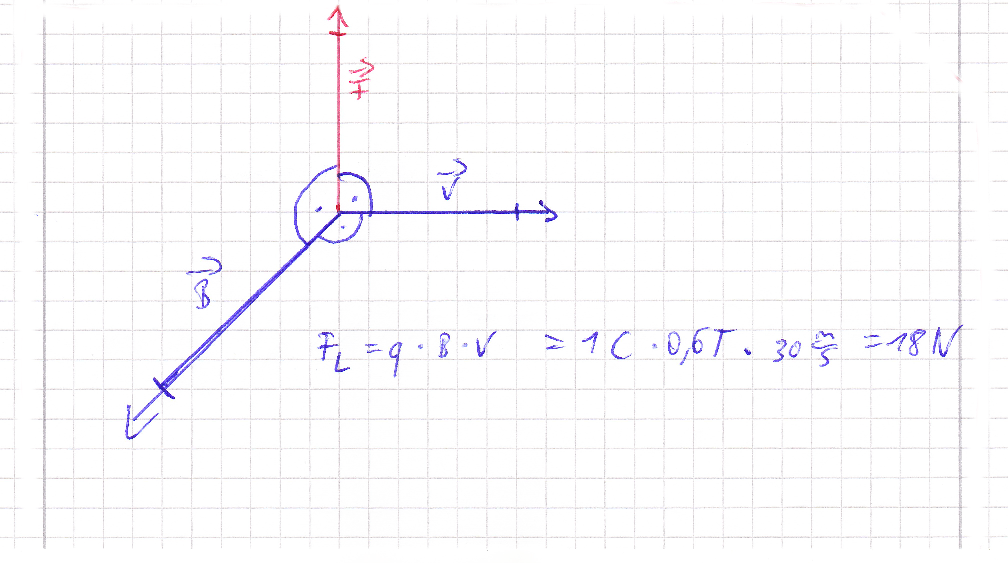
\includegraphics[scale=0.5]{24_lorentzkraft} \\
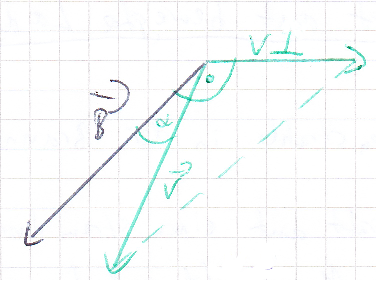
\includegraphics[scale=0.5]{24_lorentzkraft2} \\
$ F_L = q \ast \vec{v} \times \vec{B} $
\vspace{1mm} \\
$= q \ast B \ast \underbrace{v \ast sin(\alpha)} $ \\
\hspace{22.5mm} $ v \perp $

\subsection{Bewegung von Ladungen unter dem Einfluss des B-Feldes}
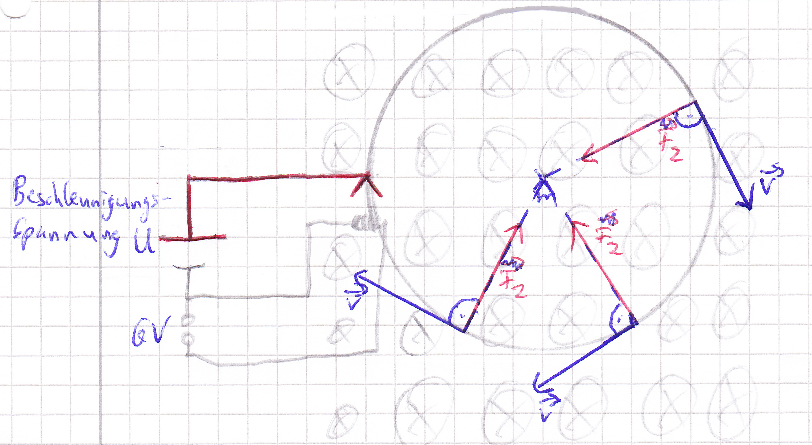
\includegraphics[scale=0.5]{25_zentripetalkraft}

\textbf{Die Lorentzkraft $F_L$ wirkt als Zentripetalkraft $F_Z$}, denn sie wirkt in jedem Punkt senkrecht zur Bewegungsrichtung und ist vom Betrag stets gleich groß. \\
Sie \underline{ändert} also ständig die \underline{Richtung der Bewegung, nicht aber} \\ den \underline{\textbf{Betrag der Geschwindigkeit!}}

\vspace{3mm} 
$ F_L = F_Z$
\vspace{1mm} \\
$ q \ast v \ast B = m \ast \frac{v^2}{r} $
\vspace{1mm} \\
$ q \ast B = m \ast \frac{v}{r} $
\vspace{2mm} \\
$ \frac{q}{m} = \frac{v}{r \ast B} $
\vspace{2mm} \\
$ \frac{e}{m} = \frac{v}{r \ast B} $

\subsubsection{Zusammenfassung: $F_L = F_Z$}
Geladene Teilchen, die mit der Geschwindigkeit $\vec{v}$ in ein homogenes $\vec{B}$-Feld senkrecht zu dessen Feldlinien eintreten, durchlaufen eine Kreisbahn mit dem Radius r. Dieser ergibt sich durch Umformung aus der zentralen Gleichung 
$F_L = F_Z$
\vspace{1mm} \\
$ q \ast v \ast B = m \ast \frac{v^2}{r} $
\vspace{1mm} \\
$ q \ast B = m \ast \frac{v}{r} $
\vspace{1mm} \\
$ r = \frac{m \ast v}{q \ast B} = \frac{v}{\frac{q}{m} \ast B} $
\vspace{5mm} \\
r ist umso größer, je
\begin{itemize}
	\item größer v ist (bei uns: U groß)
	\item kleiner B ist (bei uns: $I_{err}$ klein)
	\item kleiner die spezifische Masse ist
\end{itemize}

\subsection{B- und E-Felder im Verbund}
\subsubsection{Das Massenspektrometer}
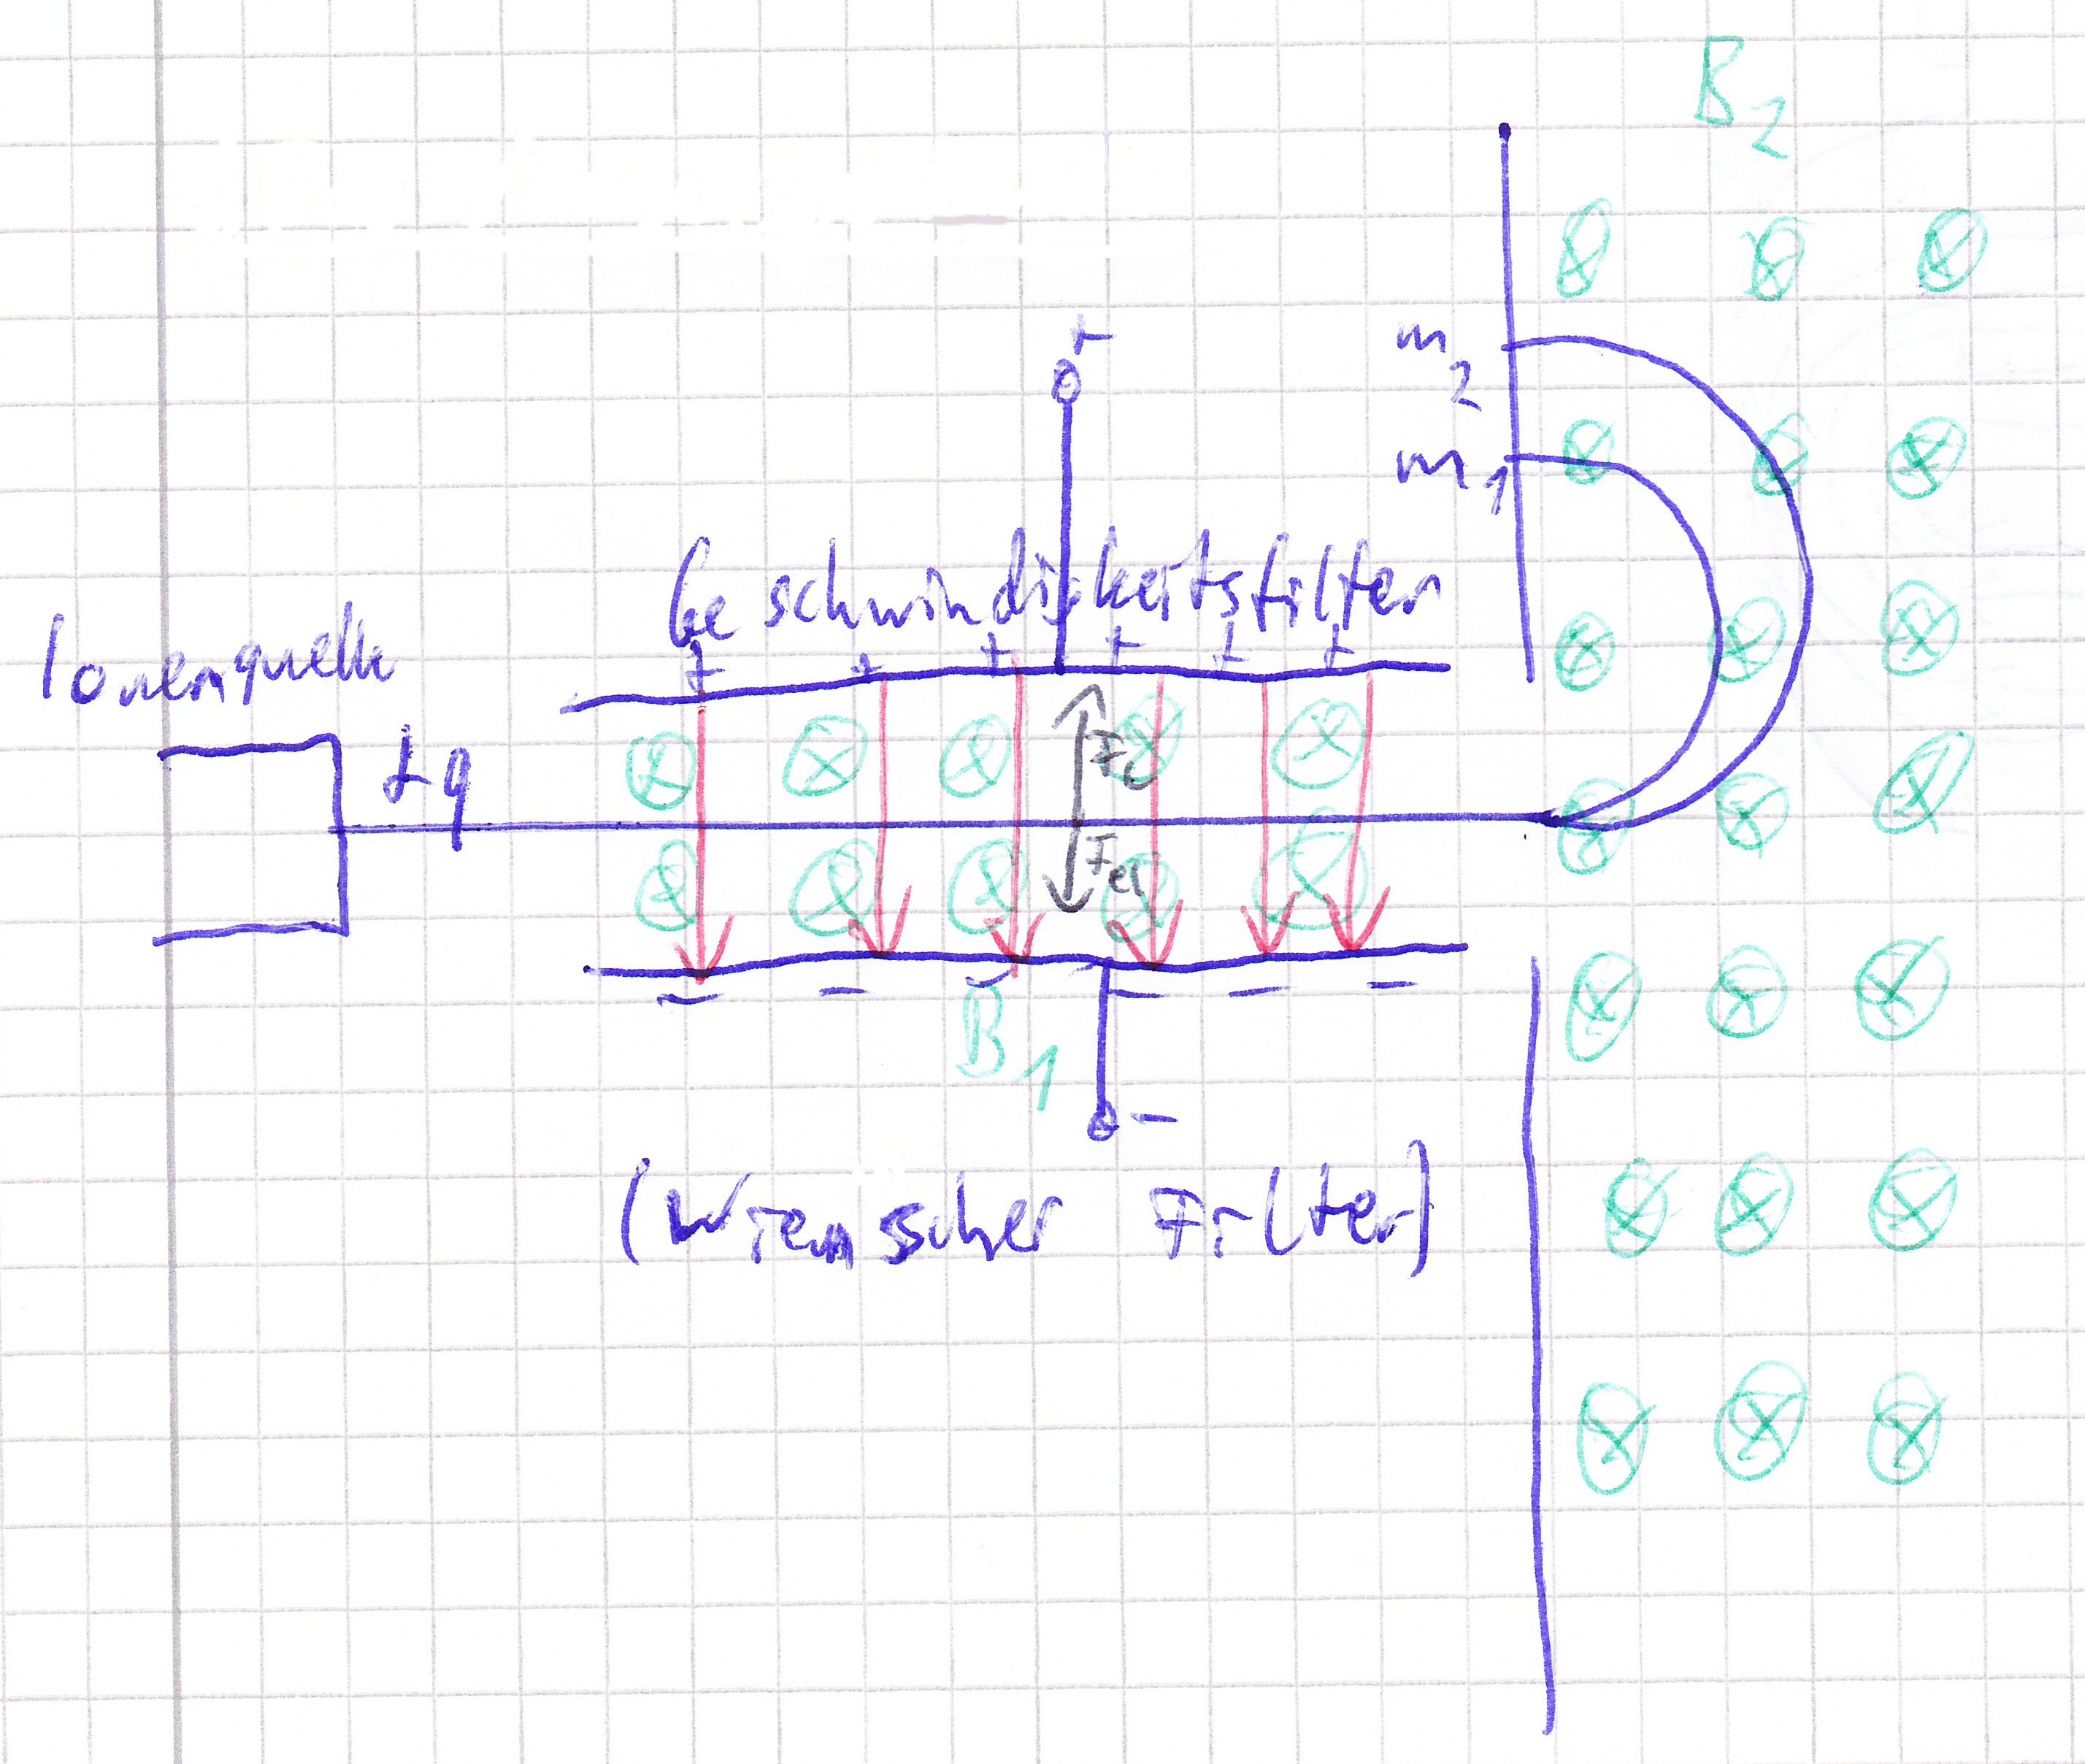
\includegraphics[scale=0.5]{261_massenspektrometer}
\newpage
\paragraph{Funktionsweise eines Wienschen Filters:} Für ein Teilchen, das die passende Geschwindigkeit hat, gilt: 
\vspace{2mm} \\
$ F_L = F_{el} $
\vspace{1mm} \\
$ q\ast v \ast B = q \ast E $
\vspace{1mm} \\
$ v \ast B = E $
\vspace{1mm} \\
$ v = \frac{E}{B} $
\vspace{5mm} \\
$ \Rightarrow $ Zu langsam: Fliegt nach unten
\vspace{1mm} \\
$ \Rightarrow $ Zu schnell: Fliegt nach oben

\paragraph{Funktion des Massenspektrometers:} Aufgrund von $r=\frac{m \ast v}{q \ast B}$ wird r für größere Massen größer ($r \sim m$), wenn alle anderen Größen konstant sind.

\subsubsection{Zyklotron}
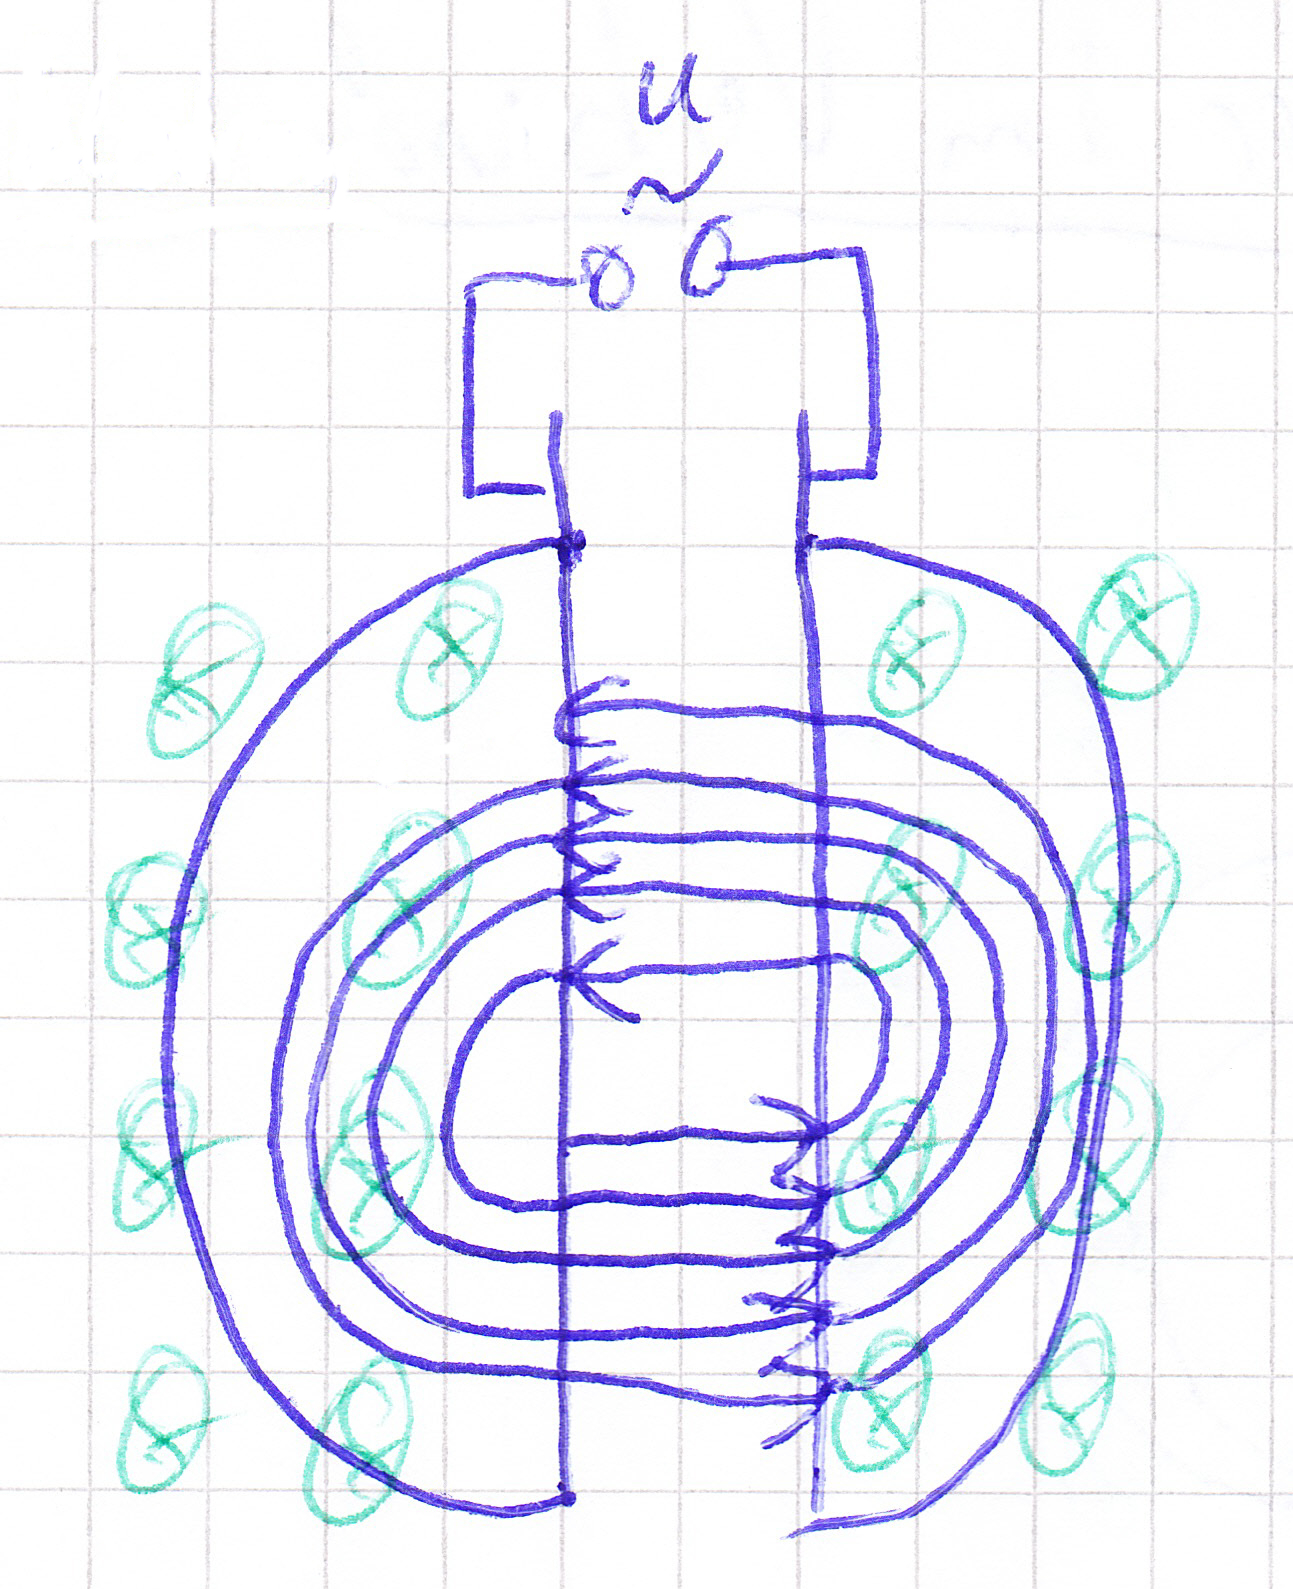
\includegraphics[scale=0.5]{262_zyklotron}

\subsection{Messung von Magnetfeldern}
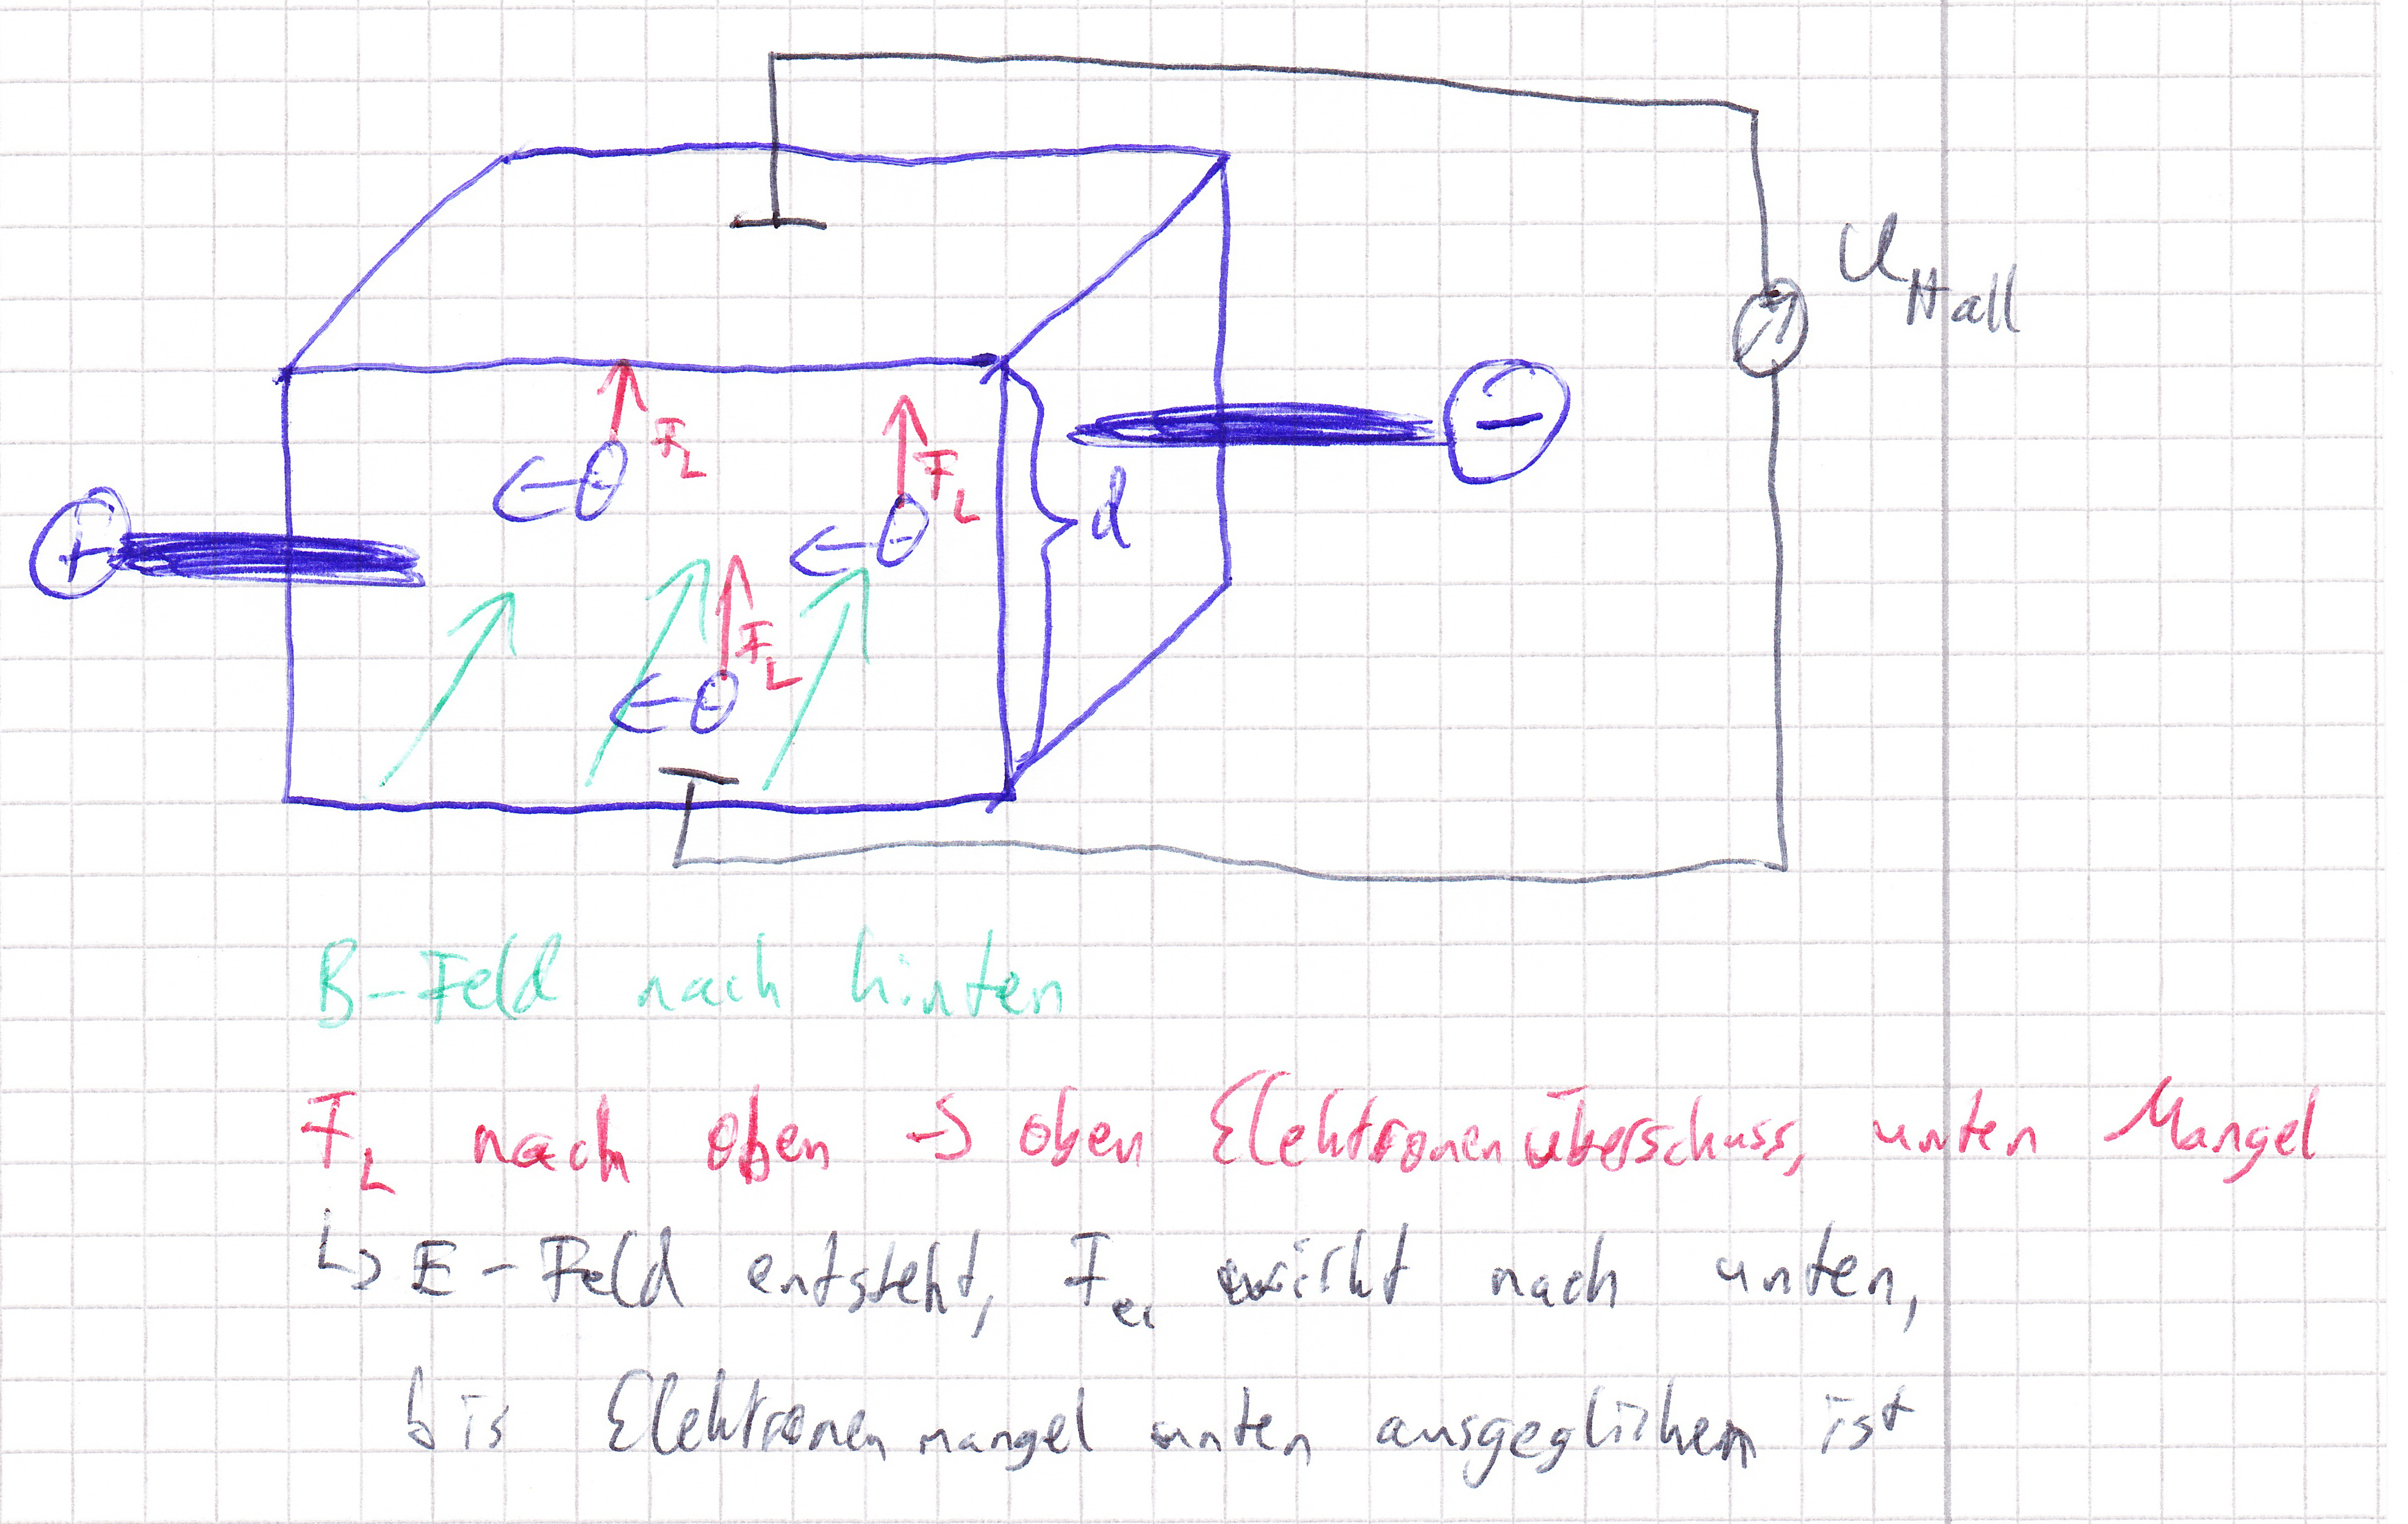
\includegraphics[scale=0.5]{27_hallsensor}\\

\begin{enumerate}
	\item Die Elektronen bewegen sich senkrecht zum B-Feld und werden deshalb nach oben abgelenkt
	\item Durch die Ladungsverschiebung \underline{entsteht} ein E-Feld, das eine $F_{el}$ auf der Elektronen nach unten ausübt.
	\item Die Ladungsverschiebung findet so lange statt, bis $F_L = F_{el}$
\end{enumerate}

Also: 
\vspace{1mm} \\
$F_L = F_{el}$
\vspace{1mm} \\
$ q \ast v \ast B = q \ast E $
\vspace{1mm} \\
$ v \ast B = E $
\vspace{1mm} \\
$ v \ast B = \frac{U}{d} $
\vspace{1mm} \\
$ U_{Hall} = B \ast v \ast d $
\vspace{5mm} 

Hall-Sonden bestehen aus Halbleitern, weil bei ihnen die Anzahl der freien Ladungsträger viel kleiner ist und somit bei gleicher Stromstärke V und damit $U_{Hall}$ größer wird.
	\section{Induktion}
	\subsection{Bewegung eines Leiters im Magnetfeld - Berechnung der Induktionsspannung}
	Bewegt sich eine Leiterschleife mit der Geschwindigkeit $v_s$ senkrecht zum Magnetfeld, wirkt auf jedes Elektron im Leiter die Lorentzkraft $F_L$.
	\begin{equation}
		F_L=e*v*B
	\end{equation}
	Sie verschiebt die Elektronen im Leiter. Dadurch wird das eine Ende des Leiters negativ geladen, das andere Ende positiv. Diese Ladungsverteilung erzeugt eine elektrische Feldstärke $E$ im Leiter, die solange anwächst, bis Gleichgewicht zwischen der Lorentzkraft und der elektrischen Kraft besteht.
		\begin{align}
		F_L&=F_el\nonumber\\
		q*v*B&=E*q\nonumber\\
		v*B&=\dfrac{U_{ind}}{d}\nonumber
		\end{align}
		\paragraph{Merke:}
		\begin{align}
		U_{ind}=v_s*B*d\\
		\intertext{mit}\nonumber\\
		v_s&=\text{Geschwindigkeit senkrecht zum Magnetfeld}\nonumber\\
		B&=\text{Magnetfeld}\nonumber\\
		d&=\text{Länge des Leiterstücks im Magnetfeld}\nonumber
		\end{align}	
	\subsection{Induktion durch Änderung der senkrecht vom Magnetfeld durchsetzten Fläche}
	Die Spule werde mit konstanter Geschwindigkeit $v_s$ in das Magnetfeld hineinbewegt.
	\paragraph{Merke:} Die induzierte Spannung $U_{ind}$ ist desto größer, je größer die Änderungsrate $\dfrac{\Delta A_s}{\Delta t}$ der senkrecht vom Magnetfeld durchsetzten Spulenfläche ist.
	\begin{subequations}
		Es gilt:
		\begin{align}
		U_{ind}&=n*B*\dfrac{\Delta A_s}{\Delta t}\nonumber\\
		&=n*B*\lim\limits_{\Delta t\rightarrow 0}  \dfrac{\Delta A_s}{\Delta t}\nonumber\\
		&=n*B*\dfrac{\mathrm{d} A_s}{\mathrm{d} t}\nonumber\\
		&=n*B*\dot{A_s}
		\end{align}
	\end{subequations}
	\subsection{Rotation einer Spule im Magnetfeld}
	Die senkrecht vom B-Feld durchsetzte Fläche ist bei einer rotierenden Spule gegeben durch:
		\begin{align}
		A(t)&=\hat{A}*cos(\omega t+\varphi_{0})\\
		\intertext{mit}
		\hat{A}&=\text{Amplitude(max. Wert der Fläche $A_s$)}\nonumber\\
		\varphi_{0}&=\text{Anfangswinkel}\nonumber\\
		\intertext{und der Winkelgeschwindigkeit}
		\omega&=\dfrac{2\pi}{T}\nonumber\\
		[\omega]&=\dfrac{1}{s}=1\text{ Hz}\nonumber\\
		\intertext{Damit erhält man:}
		\dot{A}_{(t)}&=-\hat{A}*\omega*sin(\omega t+\varphi_{0})\nonumber\\
		\intertext{Dadurch ergibt sich für die induzierte Spannung bei der Rotation einer Spule mit n Windungen im Magnetfeld B:}
		U_{ind}(t)&=n*B*\dot{A}(t)\nonumber\\
		&=-n*B*\hat{A}*\omega*sin(\omega t+\varphi_{0})\nonumber\\
		&=-\hat{U}*sin(\omega t*\varphi_{0})		
		\end{align}
	\subsection{Magnetfeldänderung}
	Induktionsspannung aufgrund der Änderung des Magnetfeldes, welches die Querschnittsfläche einer Spule $A_s$ senkrecht durchsetzt:
	\begin{align}
		U_{ind}=n*A_s*\dot{B}
	\end{align}
	\subsection{Der magnetische Fluss}
	Der magnetische Fluss ist ein Maß für die Anzahl der Feldlinien, die eine Fläche A durchsetzen.\\
	Der magnetische Fluss ist definiert als Produkt vo magnetischer Flussdichte B und dem Flächeninhalt $A_s$ der Projektion der Fläche A \underline{senkrecht} zu den Feldlinien.
	\begin{align}
	\Phi&=B*A_s\\
	[\Phi]&=T*m^2=V*s=1\text{Wb(nach Wilhelm Weber)}\nonumber
	\end{align}
	\subsection{Allgemeine mathematische Formulierung des Induktionsgesetzes}
	Wenn sich der magnetische Fluss $\Phi$ durch eine Leiterschleife so ändert, dass er die Ableitung nach der Zeit $\dot{\Phi}(t)$ hat, entsteht die Induktionsspannung
	\begin{align}
	U_{ind}&=-n*\dot{\Phi}_{(t)}\\
	\intertext{mit}
	-n&=\text{Anzahl der Spulenwindungen}\nonumber\\
	\dot{\Phi}_{(t)}&=\text{Änderungsrate des Flusses nach der Zeit}\nonumber
	\end{align}
	Erste Formulierung von Michael Faraday\\
	Wie ergeben sich daraus die betrachteten Spezialfälle:
	\begin{align*}
	U_{ind}&=-n*\dot{\Phi}_{(t)}\\
	&=-n*\dot{(A_s*B)}(t)\\
	&=-n*(\dot{A_s}*B+A_s*\dot{B})_{(t)}
	\end{align*}
	\subsection{Lenz´sche Regel- eine andere Formulierung des Energieerhaltungssatzes}
	Ein induzierter Strom $I_{ind}$ ist so gerichtet, dass das von ihm erzeugte Magnetfeld der Änderung des magnetischen Flusses entgegenwirkt, die den Strom hervorruft.\\
	Anwendung der Lenz´schen Regel:\\
	Grafik aus Ordner\\
	Die Elektronen fließen bei Annäherung des äußeren Magnetfeldes in der Leiterschleife in diese Richtung, da $B_{ind}$ die Zunahme des äußeren Magnetfeldes entgegengesetzt sein muss.
	\paragraph{Beweis der Gültigkeit des Energieerhaltungssatzes bei Induktionsvorgängen} Um den Stab mit gleichbleibender Geschwindigkeit $\vec{v}$ gegen die bremsende Lorentzkraft $F_L$ zu bewegen, muss eine Zugkraft $F_{Zug}$ aufgebracht werden, die betragsmäßig gleich, aber entgegengerichtet ist.
	Bei der Verschiebung des Stabes um $\Delta s$ nach rechts wird folgende Arbeit verrichtet:\\
	\begin{align*}
		\Delta W_{mech} &= F_{Zug}*\Delta s\\
		&=I*B*d*\Delta s\\
		&=\dfrac{U_{ind}}{R}*d*B*\Delta s\\
		&=\dfrac{B*v*d}{R}*d*B*\Delta s\\
		&=\dfrac{B^2*d^2*v}{R}*\Delta s\\
	\end{align*}
	\begin{align}
		\Delta W_{mech}&=\dfrac{B^2*d^2*v^2}{R}*\Delta t\label{Wmech}
	\end{align}
	Am Widerstand $R$, der z.B. ein elektrisches Gerät sein kann, wird in $\Delta t$ elektrische Energie umgewandelt.
	\begin{align}
		\Delta W_{el} &= \underbrace{U_{ind} * I_{ind}}_{P_{el}}*\Delta t\nonumber\\
		&=B*v*d*\dfrac{B*v*d}{R}*\Delta t\nonumber\\
		\Delta W_{el}&=\dfrac{B^2*v^2*d^2}{R}*\Delta t\label{Wel}
	\end{align}
	Aus \ref{Wmech} und \ref{Wel} folgt, dass bei Induktionsvorgängen der Energieerhaltungssatz erfüllt.\\
	Die Lenz´sche Regel ist so betrachtet nur eine andere Formulierung des Energieerhaltungssatzes.
	\subsection{Selbstinduktion}
	Eine Stromänderung in einer Spule ändert den magnetischen Fluss dieser Spule, wodurch in der Spule selbst wieder eine Spannung induziert wird. Nach der Lenz´schen Regel ist die Induktionsspannung der Stromänderung entgegengerichtet. Der Vorgang heißt Selbstinduktion.\\
	Def.: Selbstinduktion/Eigeninduktion\\
	Magnetische Rückwirkung eines sich ändernden elektrischen Stroms auf den eigenen Leiterkreis.\\
	Grafik aus Ordner\\
	\paragraph{Induktivität}
	\begin{align}
	U_{ind(t)}&=-n*A_s*\hat{B}_{(t)}\nonumber\\
	&=-n*A*\mu_0*\mu_r*\dfrac{n}{l}*\
	_{(t)}\nonumber\\
	&=\underbrace{-n^2*A*\mu_0*\mu_r*l^{-1}}_{L}*\dot{I}_{(t)}
	\intertext{$L=\mu_0*\mu_r*\dfrac{n^2}{l}*A$ heißt Induktivität der Spule}
	[L]&=\dfrac{V*s}{A}=\dfrac{\Omega}{s}=1\hspace{2mm}H\hspace{2mm}\mathrm{(Henry)}	
	\end{align}
	\paragraph{Einschaltvorgang}
	\begin{equation}
	U_{(t)}=U_1-U_{ind}=U_1-L*\dot{I}_{(t)}\nonumber
	\end{equation}
	\begin{subequations}
		\begin{align}
		I_{(t)}*R&=U_1-L*\dot{I}_{(t)}\label{dfg1}\\
		I_{(t)}&=\dfrac{U_1}{R}-\dfrac{L}{R}*\dot{I}_{(t)}\\
		\dot{I}_{(t)}&=\dfrac{U_1-I_{(t)}*R}{L}
		\intertext{Aus diesem Differentialgleichungssystem folgt:}
		\dot{I}_{(t)}&=\dfrac{R}{L}*\left( \dfrac{U_1}{R}-I(t)\right)\nonumber\\
		\rightarrow I_{(t)}&=\dfrac{U_1}{R}*\left( 1-e^{-\frac{R}{L}*t} \right)\\
		\intertext{Zum Zeitpunkt $t=0s$ gilt $I_{(0s)}=0A$}
		\rightarrow \dot{I}_{(0s)}&=\dfrac{U_1}{L}\\
		\intertext{Mit der Zunahme von $I_{(t)}$ wird $\dot{I}_{(t)}$ kleiner}
		\rightarrow \dot{I}_{\infty}&=0\frac{A}{s}\\
		\rightarrow I_{\infty}&=\dfrac{U_1}{R}	
		\end{align}
	\end{subequations}
	\paragraph{Merke:}
	\begin{enumerate}
		\item Bestimmung von $R$ aus dem Schaubild:\\
		\subitem 	\begin{equation}
						R=\dfrac{U_1}{I_{\infty}}
					\end{equation}
		\item Bestimmung von $L$ aus dem Schaubild:\\
		\subitem $\dot{I}_{0s}$ bestimmen;
		\subitem 	\begin{equation}
						L=\dfrac{U_1}{\dot{I}_{0s}}
					\end{equation}
		\item für größeres $L$ (z.B. Eisenkern):
		\subitem verzögerter Anstieg,
		\subitem Schranke bleibt gleich
		\subitem $\rightarrow$ "wird flacher"
		\item  für größeres $R$:
		\subitem Schranke wird niedriger
		\subitem schnellerer Anstieg
		\subitem $\dot{I}_{0s}$ ist gleich
	\end{enumerate}
	\paragraph{Ausschaltvorgang}
	Beim Ausschaltvorgang verhindert die Spule ein sofortiges Zusammenbrechen des Stroms.
	\begin{align}
	\intertext{aus \ref{dfg1} folgt:}
	I_{(t)}*R&=0-L*\dot{I}_{(t)}\nonumber\\
	\dot{I}_{(t)}&=-\dfrac{R}{L}*I_{(t)}
	\intertext{Lösungsfunktion:}
	I_{(t)}&=I_{\infty}*e^{-\frac{R}{L}*t}\nonumber\\
	&=\dfrac{U_1}{R}*e^{-\frac{R}{L}*t}
	\end{align}
	\paragraph{Verzweigter Stromkreis}
	Grafiken im Ordner
	\subsection{Leistung und Energie im Magnetfeld}
	Nach Abschalten der äußeren Spannung $U_{1}$ rührt der Strom $I_{(t)}=I_{ind(t)}$ ausschließlich von der Spannung $U_{ind(t)}$ her. Daraus ergibt sich für die Leistung:
	\begin{align}
		P_{(t)}&=U_{(t)}*I_{(t)}\nonumber\\
		\intertext{hier:}
		&=U_{ind(t)}*I_{ind(t)}\nonumber\\
		&=-L*\dot{I}_{(t)}*I_{(t)}
	\end{align} 
	Die Gesamtenergie, die in der Spule gespeichert ist, ist das Integral der Funktion $W_{mag}=\int_{t_0}^{\infty}P\mathrm{d}t$
	\begin{align}
	W_{mag}&=\int_{t_0}^{\infty}-L*\dot{I}_{(t)}*I_{(t)}\mathrm{d}t\nonumber\\
	%&=\sideset{}{_{t_0}^{\infty}}{\left[-\frac{1}{2} L*I^2_{(t)}\right]}\nonumber\\
	&=0+\frac{1}{2}*L*I^{2}_{(0)}\nonumber
	\intertext{Die Energie, die im Feld einer stromdurchflossenen Spule gespeichert ist, berechnet sich allgemein aus:}
	W_{mag}&=-\frac{1}{2}*L*I^2
	\intertext{Die Energiedichte im magnetischen Feld $\rho_{mag}$ berechnet sich demnach aus:}
	\rho_{mag}&=\frac{W_{mag}}{V}\nonumber\\
	&=\frac{\frac{1}{2}*\mu_0*\mu_r*\frac{n^2}{l}*A*I^2}{V}\nonumber\\
	&=\frac{1}{2}\frac{B^2}{\mu_0*\mu_r}
	\end{align}
	\subsection{Die Maxwell´schen Gleichungen}
	\begin{subequations}
		Elektrische Ladungen sind die Quellen und Senken der elektrischen Feldlinien
		\begin{align}
		\oint E\mathrm{d}A=\dfrac{Q}{\epsilon_0}
		\end{align}
		Der gesamte magnetische Fluss durch jede beliebige geschlossene Fläche ist 0.
		\begin{align}
		\oint B\mathrm{d}A=0
		\end{align}
		Die Änderung der magnetischen Flussdichte, die eine Fläche durchsetzt, erzeugt ein elektrisches Wirbelfeld um diese Fläche herum
		\begin{align}
			\oint E\mathrm{d}l=-\dfrac{d}{dt}\oint BdA
		\end{align}
		Ein stromdurchflossener Leiter erzeugt um den Leiter herum ein magnetisches Wirbelfeld. Eine zeitliche Änderung des elektrischen Feldes, das eine Fläche durchsetzt, erzeugt um die Fläche herum ein magnetisches Wirbelfeld
		\begin{align}
			\oint B\mathrm{d}l=\mu_0 *I+\mu_0 \epsilon_0\dfrac{d}{dl} \oint EdA
		\end{align}
	\end{subequations}
	\section{Schwingungen}
	\subsection{Schwingungsvorgänge und Schwingungsgrößen}
	\paragraph{Merkmale einer Schwingung}
	\begin{enumerate}
		\item Die Bewegung verläuft periodisch
		\item Die Bewegung verläuft zwischen 2 Umkehrpunkten und durch einen ausgezeichneten Punkt, die Ruhelage oder Gleichgewichtslage des Oszillators
	\end{enumerate}
	\paragraph{Entstehung einer Schwingung}
	\begin{enumerate}
		\item Auslenkung des Oszillators aus der Ruhelage (Energiezufuhr)
		\item Das Vorhandensein einer zur Gleichgewichtslage zurücktreibenden Kraft $F_R$ (Rückstellkraft)
		\item Die Trägheit des Oszillators aufgrund derer er sich über die Gleichgewichtslage hinausbewegt
	\end{enumerate}
	\paragraph{Schwingungsgrößen}
	\begin{enumerate}
		\item Periodendauer $T$
		\begin{equation*}
			T=\frac{t}{n}
		\end{equation*}
		(t Zeit für n Schwingungen)
		\item Frequenz $f$
		\begin{equation*}
			f=\frac{1}{T}
		\end{equation*}
		 $[f]=1Hz$
		 \item Auslenkung aus der Ruhelage Elongation $s(t)$
		 \item Die \underline{Amplitude} ist die größte Elongation $\hat{s}$
	\end{enumerate}
	\subsection{harmonische und nichtharmonische Schwingungen}
	Eine Schwingung, deren Zeit-Weg-Diagramm eine Sinuskurve ergibt, heißt harmonische Schwingung.
	\paragraph{Bewegungsgleichung einer harmonischen Schwingung}
	\begin{align*}
	&s(t)=\hat{s}*sin(\omega t+\varphi_{0})\\
	&v(t)=\dot{s}(t)=\hat{s}*\omega*cos(\omega t+\varphi_{0})\\
	&a(t)=\dot{v}(t)=-\hat{s}*\omega^{2}*sin(\omega t+\varphi_{0})
	\end{align*}

	\subsection{Zusammenhang zwischen Kraft und Auslenkung: Wiederholung des \underline{Hookeschen Gesetzes}}
	\paragraph{Federpendel}
	Die stets zur Ruhelage hin wirkende resultierende Kraft heißt rücktreibende Kraft$F_R$.\newline Beim Federpendel gilt das lineare Kraftgesetz:
	\begin{equation*}
		F_{R}=-D*s
	\end{equation*}
	\paragraph{Der horizontale Federschwinger}
	Aus dem Versuch folgt das allgemeine lineare Kraftgesetz:
	\begin{equation*}
		F_{R}=-(D_1+D_2)*s
	\end{equation*}
	
	\subsection{Das Kraftgesetz der harmonischen Schwingung}
	\paragraph{Von der Bewegungsgleichung der harmonischen Schwingung zum linearen Kraftgesetz}
	\begin{equation}\label{Bewegungsgleichung der harmonischen Schwingung}
		s(t)=\hat{s}*sin(\omega t+\varphi_{0})
	\end{equation}
	Außerdem gilt:
	\begin{equation}\label{F=m*a}
		F=m*a(t)=m*\ddot{s}(t)
	\end{equation}
	Aus Gleichung \ref{Bewegungsgleichung der harmonischen Schwingung} und \ref{F=m*a} folgt:
	\begin{subequations}
		\begin{align}\label{Harmonie-->Linearität}
			F(t) &=m*(-\hat{s}*\omega^{2}*sin(\omega t+\varphi_{0}))\\
			&= -m*\omega^{2}*\hat{s}*sin(\omega t+\varphi_{0})\\
			&= -m*\omega^{2}*s(t)\\
			&= -D*s(t)
		\end{align}
	\end{subequations}
	Gleichung \ref{Harmonie-->Linearität} ist also gleichbedeutend mit folgender Implikation:\newline
	Schwingung verläuft harmonisch $\rightarrow$ die zugrunde liegende Kraft muss dem linearen Kraftgesetz gehorchen.
	\paragraph{Vom linearen Kraftgesetz zur Bewegungsgleichung der harmonischen Schwingung}
	\begin{subequations}\label{harmonische Schwingung-->lineares Kraftgesetz}
		\begin{align}
		F(t)&=-D*s(t)\\
		m*a(t)&=-D*s(t)\\
		m*\ddot{s}(t)&=-D*s(t)
		\end{align}
		Differentialgleichung zweiter Ordnung
		\begin{align}
		\ddot{s}(t)=-\dfrac{D}{m}*s(t)\label{dgl}
		\end{align}
		Die Lösungsfunktion, die diese Differentialgleichung löst, lautet:
		\begin{align}
		s(t)&=\hat{s}*sin(\sqrt{\dfrac{D}{m}}*t+\varphi_{0})\\
		&=\hat{s}*sin(\omega*t+\varphi_{0})
		\end{align}
		Es gilt: $\omega=\sqrt{\dfrac{D}{m}}$
		\begin{align}
		\dot{s}(t)&=\hat{s}*\sqrt{\dfrac{D}{m}}*cos(\sqrt{\dfrac{D}{m}}*t+\varphi_{0})\\
		\ddot{s}(t)&=-\hat{s}*\dfrac{D}{m}*sin(\sqrt{\dfrac{D}{m}}*t+\varphi_{0})\\
		&=\underbrace{-\omega^{2}*\hat{s}}_{a} *sin(\omega t+\varphi_{0})\\
		&=-\dfrac{D}{m}*s(t)\label{lineares Kraftgesetz}
		\end{align} 
	\end{subequations}
	Gleichungssystem \ref{harmonische Schwingung-->lineares Kraftgesetz} ist also gleichbedeutend mit folgender Implikation:\newline
	Ein lineares Kraftgesetz gilt $\rightarrow$ Die Schwingung verläuft harmonisch
	\subparagraph{Merke:}
	Damit s(t) Lösungsfunktion der Differentialgleichung \ref{dgl} ist, muss gelten:
	\begin{subequations}
		\begin{align}
		\omega&=\sqrt{\dfrac{D}{m}}\\
		&=\dfrac{2\pi}{T}\\
		&=2*\pi*f
		\end{align}
		\begin{align}
		\hat{v}&=\hat{s}*\omega\\
		\hat{a}&=\hat{s}*\omega^2
		\end{align}
	\end{subequations}
	\textbf{Lineares Kraftgesetz $\leftrightarrow$ Die Schwingung ist harmonisch}
	\subsection{Das Fadenpendel}
	\begin{align}
	\dfrac{F_R}{F_G}&=sin(\varphi)\nonumber\\
	F_R&=F_G*sin(\varphi)\nonumber\\
	&=F_G*sin(\dfrac{s}{l})\nonumber\\
	&=m*g*sin(\dfrac{s}{l})\nonumber\\
	\intertext{Mit Taylorreihennäherung dürfen wir für $-30^\circ\le\varphi\le 30^\circ$ annehmen:}
	F_R&=m*g*\dfrac{s}{l}\nonumber\\
	&=\underbrace{\dfrac{m*g}{l}}_{D}*s
	\end{align}
	Dann hätten wir eine harmonische Schwingung mit dem Zeit-Elongations-Gesetz $s(t)=\hat{s}*sin(\omega t+\varphi_{0})$ mit: 
	\begin{align*}
	\omega&=\sqrt{\dfrac{D}{m}}=\sqrt{\dfrac{\dfrac{m*g}{l}}{m}}=\sqrt{\dfrac{g}{l}}\\
	T&=s*\pi*\sqrt{\dfrac{m}{D}}=2*\pi*\sqrt{\dfrac{g}{l}}
	\end{align*}
	\subsection{Energie der harmonischen Schwingung}
	\begin{align}
		W_{pot}&=\int F\mathrm{d}s\nonumber\\
		W_{pot(s)}&=\frac{1}{2}*D*s^2\nonumber\\
		W_{pot(s)}&=\frac{1}{2}*D*\hat{s}^2
	\end{align}
	Die potenzielle Energie $W_{pot}$ errechnet sich aus der Energie, die beim Verschieben des Schwingers aus der Gleichgewichtslage bis zur augenblicklichen Auslenkung s gegen die rücktreibende Kraft $F_R=-D*s$ zuzuführen ist:\\
	$W_{pot}=\frac{1}{2}*D*s^2$
	Die kinetische Energie des harmonischen Oszillators zu einem beliebigen Zeitpunkt $t$ ergibt sich aus $W_{kin}=\frac{1}{2}*m*v^2$.\\
	\begin{subequations}
		Für $s(t)=\hat{s}*sin(\omega t)$ ergibt sich für $W_{pot}$:
		\begin{align}
		W_{pot}&=\frac{1}{2}*D*s_{(t)}\nonumber\\
		&=\frac{1}{2}*D*\hat{s}^2*sin^2(\omega t)\label{wpot2}
		\intertext{und für $W_{kin}$:}
		W_{kin}&=\frac{1}{2}*m*(\hat{s}^2*\omega^2)*cos^2(\omega t)\nonumber\\
		\intertext{mit}
		\omega^2&=\dfrac{D}{m}\nonumber\\
		\intertext{Dies lässt sich vereinfachen zu:}
		W_{kin}&=\frac{1}{2}*D*\hat{s}^2*cos^2(\omega t)\label{wkin2}
		\intertext{Aus \ref{wpot2} und \ref{wkin2} folgt:}
		W_{ges}&=\frac{1}{2}*D*\hat{s}^2*sin^2(\omega t)+\frac{1}{2}*D*\hat{s}^2*cos^2(\omega t)\nonumber\\
		&=\frac{1}{2}*D*\hat{s}^2*(sin^2(\omega t)+cos^2(\omega t))\nonumber\\
		W_{Ges}=\frac{1}{2}*D*\hat{s}^2
		\end{align}
	\end{subequations}
	\pagebreak
	\subsection{Die gedämpfte harmonische Schwingung}
	Jede freie Schwingung ist gedämpft, da der Oszillator Energie an die Umgebung abgibt.
	\paragraph{Dämpfung bei konstanter Kraft}
	gedämpfte Sinuskurve(Heft)
	\begin{align}
	\frac{1}{2}*D*\hat{s}_{0}^2-\frac{1}{2}*D*\hat{s}_{1}^2&=F_{reib}*(\hat{s}_0+\hat{s}_1)\nonumber\\
	\frac{1}{2}*D(\hat{s}_0^2-\hat{s}_1^2)&=F_{reib}*(\hat{s}_0+\hat{s}_1)\nonumber\\
	\frac{1}{2}*D*(\hat{s}_0-\hat{s}_1)*(\hat{s}_0+\hat{s}_1)&=F_{reib}*(\hat{s}_0+\hat{s}_1)\nonumber\\
	\frac{1}{2}*D*(\hat{s}_0-\hat{s}_1)&=F_{reib}\nonumber\\
	\hat{s}_0-\hat{s}_1&=\dfrac{2*F_{reib}}{D}
	\end{align}
	Bei der konstanten Reibungskraft $F_{reib}$ nehmen die Amplituden linear ab, d.h. die Amplituden verringern sich von Umkehrpunkt zu Umkehrpunkt stets um den selben Betrag.\\
	Es gilt:
	\begin{align}
		m*\ddot{s}_{(t)}=-D*s-F_{reib}
	\end{align}
	\paragraph{Dämpfung durch eine zur Geschwindigkeit proportionale Kraft}
	\begin{align}
		m*\ddot{s}_{(t)}=-D*s_{(t)}-k*\dot{s}_{(t)}
	\end{align}
	Bei der Lösungsfunktion gilt, dass $\dfrac{\hat{s}_0}{\hat{s}_1}=\dfrac{\hat{s}_1}{\hat{s}_2}=\dfrac{\hat{s}_2}{\hat{s}_3}=const$.
	\begin{align}
	\intertext{Aufgabe:\hspace{2mm}Lösung der Differentialgleichung}
	m*\ddot{s}_{(t)}&=-D*s_{(t)}-k*\dot{s}_{(t)}\nonumber\\
	m*\ddot{s}_{(t)}+k*\dot{s}_{(t)}+D*s_{(t)}&=0\\
	\intertext{Annahme:\hspace{2mm}$s_{(t)}=e^{xt}$}
	m*x^2*e^{xt}+k*x*e^{xt}+D*e^{xt}&=0\nonumber\\
	\left(m*x^2+k*x+D\right)*e^{xt}&=0\nonumber\\
	\rightarrow m*x^2+k*x+D&=0
	\intertext{Diese quadratische Gleichung hat die Lösungen:}
	x_1&=\frac{-k+\sqrt{k^2-4*m*D}}{2m}\nonumber\\
	x_2&=\frac{-k-\sqrt{k^2-4*m*D}}{2m}\nonumber
	\end{align}
	Für die Lösungsfunktion der Differentialgleichung folgt also:
	\begin{align}
	s(t)&=\frac{m*\ddot{s}_{(t)}+k*\dot{s}_{(t)}}{-D}\nonumber\\
	&=\frac{m*\left(e^{xt}\right)+k*\left(e^{xt}\right)}{-D}\nonumber\\
	\intertext{Möglichkeit\hspace{2mm}1:}
	&=\frac{m*e^{\frac{-k+\sqrt{k^2-4*m*D}}{2m}t}+k*e^{\frac{-k+\sqrt{k^2-4*m*D}}{2m}t}}{-D}
	\intertext{Möglichkeit\hspace{2mm}2:}
	&=\frac{m*e^{\frac{-k-\sqrt{k^2-4*m*D}}{2m}t}+k*e^{\frac{-k-\sqrt{k^2-4*m*D}}{2m}t}}{-D}	
	\end{align}
	\paragraph{Dämpfung durch den Luftwiderstand}
	\begin{align}
		m*\ddot{s}_{(t)}=-D*s_{(t)}-b*\dot{s}_{(t)}^{\hspace{2mm}2}
	\end{align}
	\subsubsection{Einschub: Tacoma Bridge}
	\begin{itemize}
		\item Datum: 7. November 1940
		\item Name: Tacoma Narrows Bridge
		\item Spannweite: 853 m
		\item Zwei in 37 m tiefem Wasser stehende Pylone
		\item Windgeschwindigkeit: 68 km/h
		\item Amplitude: 0.6 m 
	\end{itemize}
	\subsection{Erzwungene Schwingungen}
	Überlässt man einen Oszillator nach dem Anstoßen sich selbst, so schwingt er mit der Eigenfrequenz $f_0$ (bzw. $\omega_0=s\pi*f_0$)\\
	Wenn auf einen Schwinger periodisch eine Kraft $F_1=\hat{F_1}*sin(\omega_{Err}*t)$ ausgeübt wird, führt er eine erzwungene Schwingung aus. Er schwingt dann mit der Frequenz des Erregers $f_{Err}$.\\
	\underline{Resonanz} tritt auf, wenn $f_{Err}=f_0$.\\
	Die Differentialgleichung der Schwingung lautet hier:\\
	\begin{align}
		m*\ddot{s}_{(t)}=-D*s_{(t)}-k*\dot{s}_{(t)}+\hat{F_1}*sin(\omega_{Err}*t)
	\end{align}
	Im Resonanzfall beträgt die Phasendifferenz zwischen Erreger und Oszillator $\dfrac{\pi}{2}$!\\
	Der Oszillator nimmt besonders viel Energie auf!
	\section{Wellen}
\subsection{Definition}
\paragraph{Beispiele:} Elektromagnetische Wellen (Radio, Licht...), Schallwelle, Wasserwelle, Erdbebenwelle... 

\paragraph{Welle:} 
Ein sich räumlich fortpflanzender Bewegungszustand, der \underline{Energie}, aber \underline{keine Materie} transportiert.

\paragraph{Wellenausbreitung im Medium:}
Jeder Oszillator ist an seine Nachbarn gekoppelt und wird zu einer erzwungenen Schwingung angeregt.

\vspace{2mm}
\underline{Skizze}\\
Das 3. Teilchen beschleunigt das 4. Teilchen und erfährt die reactio. Die Ausbreitung erfolgt umso schneller, je größer D und je kleiner m ist ($a = \dfrac{F}{m}$)

\subsection{Wichtige physikalische Größen}
Während ein einzelner Oszillator eine Schwingung (mit der Periodendauer T) vollführt, ist die Welle gerade eine Wellenlänge $\lambda$ weiter vorgerückt. \\
Also beträgt die Ausbreitungsgeschwindigkeit c der Welle
\vspace{2mm} \\
$ c = \dfrac{\lambda}{T} = \lambda \ast f $

\vspace{2mm}
Die Geschwindigkeit jedes einzelnen Oszillators v bei der erzwungenen Schwingung wird - zur Unterscheidung von der Ausbreitungsgeschwindigkeit c - ab jetzt mit \underline{Schnelle v} bezeichnet.
\vspace{2mm} \\
\paragraph{Transversalwelle:} 
Bei einer Transversalwelle steht der Schwingungsvektor \underline{senkrecht} zur Ausbreitungsrichtung. Wellenberge und Wellentäler laufen über den Wellenträger. \\
Bsp.: elektromagnetische Wellen, S-Wellen beim Erdbeben. \\
\underline{Mechanische} Transversalwellen können nur entstehen, wenn zwischen den Oszillatoren \underline{elastische Querkräfte} wirksam sind (also nur im Festkörper).

\paragraph{Longitudinalwelle:} 
Bei einer Longitudinalwelle steht der Schwingungsvektor \underline{parallel} zur Ausbreitungsrichtung. \underline{Verdichtungen} und \underline{Verdünnungen} laufen über den Wellenträger. \\
Bsp.: Schallwellen, Wasserwellen, P-Wellen beim Erdbeben. \\
Longitudinalwellen können dann entstehen, wenn zwischen den Oszillatoren Kräfte wirksam sind, die der Volumenänderung entgegenwirken.\\
\underline{Mechanische} Longitudinalwellen sind "Druckwellen" (existieren in Festkörper, Flüssigkeiten und Gasen) \\
Zur Skizze: $\overrightarrow{v} \perp \overrightarrow{c}$ \\
Zur Skizze 2: $\overrightarrow{v} \parallel \overrightarrow{c}$ \\
\underline{Skizzen RS zu AB10.04. } \\
Die Ausbreitungsgeschwindigkeit c wird auch \underline{Phasen}geschwindigkeit ($v_{ph}$) genannt, weil sie die Geschwindigkeit ist, mit der sich eine bestimmte Phasenlage der Oszillation über den Wellenträger ausbreitet.

\subsection{Zeitliche und räumliche Darstellung einer Welle}
\underline{Zeichnung zeitl, Darstellung RS zu AB10.04. }
\vspace{2mm} \\
Beim "zeitlichen Durchblick" ist der zeitliche Verlauf der erzwungenen Schwingung an einem Ort dargestellt. \\
Beim "räumlichen Durchblick" zu einem Zeitpunkt t stellt sich die Welle dar, wie man sie zu diesem Zeitpunkt im Raum sieht (Fotografie). Der Oszillator am Kopf der Welle beginnt gerade zu diesem Zeitpunkt seine Schwingung, sein Nachbaroszillator schwingt bereits einen kurzen Moment, dessen Nachbaroszillator schwingt noch einen Moment länger etc. Man sieht alle Phasenzustände nebeneinandergelegt. \\
Beim "diagonalen Durchblick" verfolgt man eine bestimmte Schwingungsphase (Zum Beispiel den Kopf der Welle oder den ersten Wellenberg) bei seiner Wanderung über den Wellenträger.

\subsection{Die Bewegungsgleichung einer Welle}
1. Der Oszillator am Punkt x=0, der zum Zeitpunkt t=0s von der Welle erfasst wird, hat die Bewegungsgleichung $ s_{(0cm, t)} = \hat{s} \ast sin(\omega \ast t) $ 
\vspace{2mm} \\
2. Der Oszillator am Punkt x, der zum Zeitpunkt $ t = \frac{x}{c} $ von der Welle erfasst wird, hat die Bewegungsgleichung $ s_{(x, t)} = \hat{s} \ast sin(\omega \ast t - \dfrac{2 \pi}{T} \ast \dfrac{x}{c})  = \hat{s} \ast sin(\omega \ast (t - \dfrac{x}{c})) $ 
\vspace{3mm} \\
$ s_{(x,t)} $ ist eine "doppelt-periodische" Funktion. Für konstantes x ist die Periode die Schwingungsdauer T, für konstantes t ist die Periode die Wellenlänge $\lambda$. 
\vspace{2mm} \\
Die Bewegungsgleichung ist die Lösungsfunktion der Differentialgleichung der Welle: \\ $ F_{(x,t)} = m \ast \ddot{s}_{(x,t)} $ \\
Die Kraft auf einen Oszillator ist proportional zur Krümmung der Kurve $ s_{(x,t)} $ 
\vspace{2mm} \\
$ F_{(x,t)} = D \ast s''_{\hspace{1,5mm}(x,t)} $ 
\vspace{2mm} \\
$ D \ast s''_{\hspace{1,5mm}(x,t)} = m \ast \ddot{s}_{(x,t)} $	
\vspace{2mm} \\
Kontrolle: Einsetzen von $s_{(x,t)} = \hat{s} \ast sin(\omega \ast t - \frac{2\pi}{\lambda} \ast x) $
\vspace{3mm} \\
$ D \ast (-\hat{s} \ast (\frac{2\pi}{\lambda})^{2} \ast sin(\omega \ast t - \frac{2\pi}{\lambda} \ast x)) = m \ast (-\hat{s} \ast \omega^{2} \ast sin(\omega \ast t - \frac{2\pi}{\lambda} \ast x)) $
\vspace{2mm} \\
$ D \ast (\frac{2\pi}{\lambda})^{2} = m \ast \omega^{2} $ 
\vspace{2mm} \\
$ D \ast (\frac{2\pi}{\lambda})^{2} = m \ast (\frac{2\pi}{\lambda})^{2} $
\vspace{2mm} \\
$ D \ast \frac{1}{\lambda{2}} = m \ast \frac{1}{T^{2}} $
\vspace{2mm} \\
$ \frac{D}{m} = \frac{\lambda{2}}{T^{2}} = c^{2} $
\vspace{2mm} \\
$ c = \sqrt{\frac{D}{m}} $	

\paragraph{Zeigerdarstellung:} Jedem Oszillator am Ort x kann ein Zeiger zugeordnet werden, der gegen den Uhrzeigersinn rotiert und dessen y-Komponente die momentane Elongation $s_{(x,t)}$ angibt. 

\newpage

\subsection{Einschub: Überlagerung zweier harmonischer Schwingungen an einem Ort}
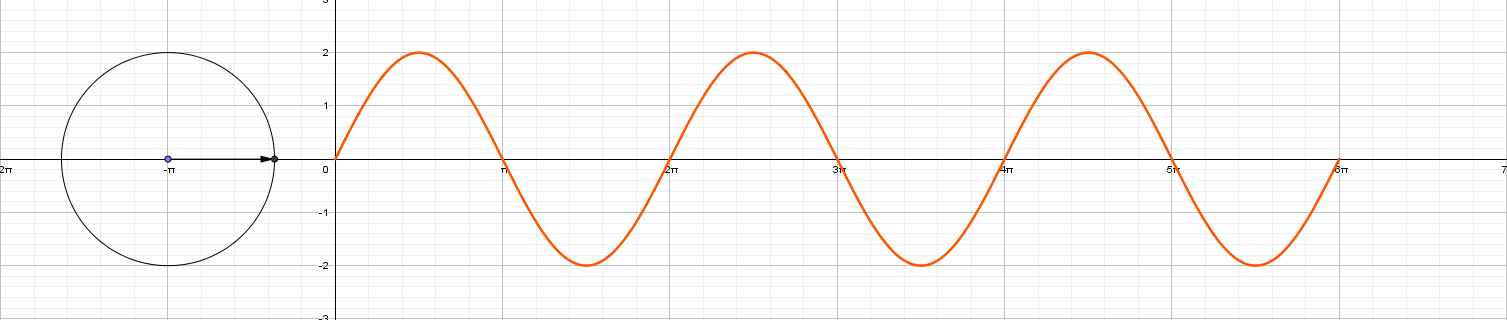
\includegraphics[scale=0.426]{sin6_1}
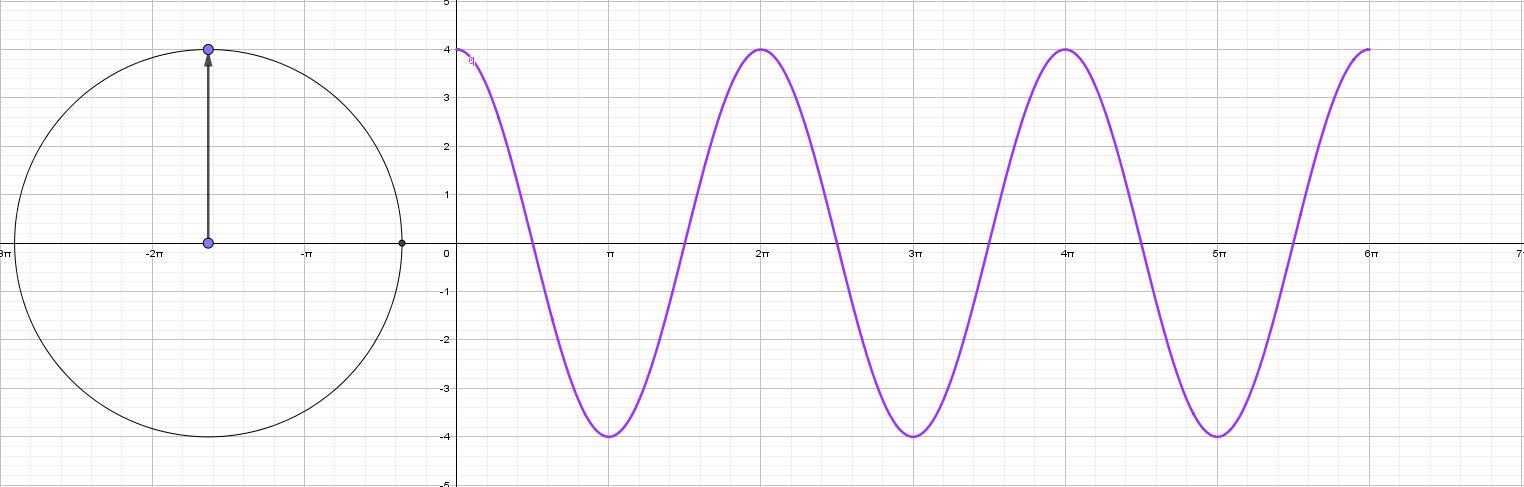
\includegraphics[scale=0.421]{sin6_2}
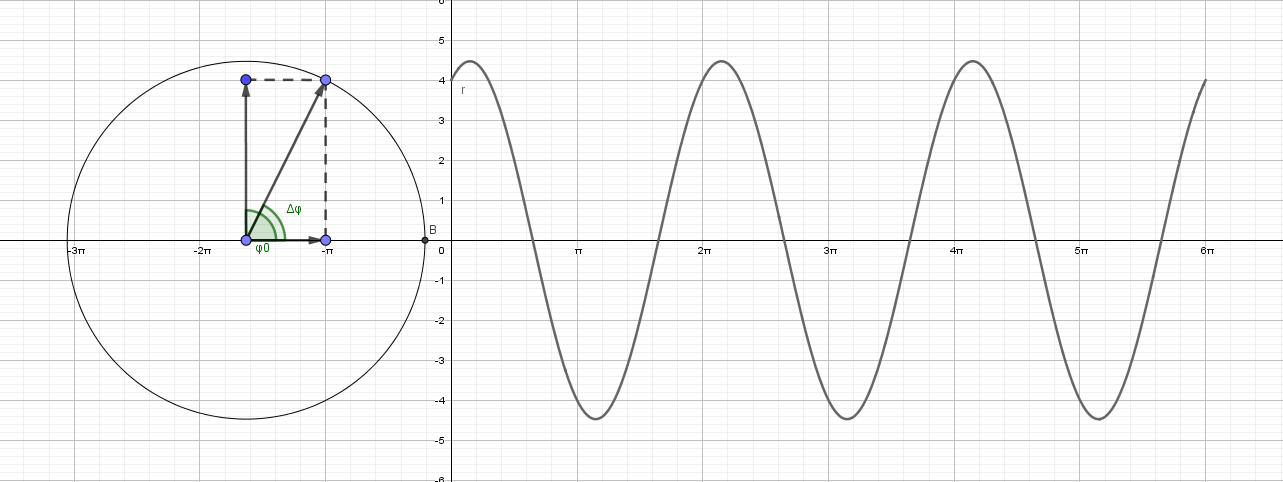
\includegraphics[scale=0.5]{sin6_3}
\vspace{2mm} \\
Die Zeiger von $s_{1}$ und $s_{2}$ rotieren mit der gleichen Winkelgeschwindigkeit $\omega$ gegen den Uhrzeigersinn. Ihre relative Lage zueinander bleibt dabei immer gleich. Das Zeigerdiagramm ermöglicht es uns, durch die vektorielle Addition der Zeiger von $s_{1}$ und $s_{2}$ den resultierenden Zeiger $s_{res}$zu bestimmen. Die Länge des resultierenden Zeigers entspricht $\hat{s}_{res}$, die Phasendifferenz $\Delta \varphi$ bezüglich z.B. $s_{1}$ gibt an, um welche Phase der Schwingung $s_{res}$ gegenüber $s_{1}$ vorauseilt. Zudem erhält man die aktuelle Phasenlage des Zeigers für den Zeitpunkt, den das Zeigerdiagramm darstellt. 
\newpage

\subsection{Überlagerung von Wellen - Allgemeines Prinzip}
\paragraph{Prinzip der ungestörten Überlagerung von Wellen:}
Treffen an einer Stelle eines Wellenträgers mehrere Wellen aufeinander, so addieren sich dort die Elongationen und Schnellen der Schwingungen. Nach dem Zusammentreffen laufen die Wellen ungestört weiter. \\
Die ungestörte Überlagerung mehrerer Wellen von gleicher Frequenz (gleicher Wellenlänge) wird als Interferenz bezeichnet.

\subsection{Interferenz}
\subsubsection{Überlagerung gleich laufender Wellen}
Bei Interferenz zweier Wellen gleicher Frequenz ergibt sich \\
1. konstruktive Interferenz (maximale Verstärkung) bei einer Phasendifferenz von $\Delta \varphi = 0$ oder $\Delta \varphi = k \ast 2 \pi $, entsprechend einem Gangunterschied von $ \delta = 0 $ oder $ \delta = k \ast \lambda $ mit k = 1,2,3,... $(k \in \mathbb{N})$ \\
2. destruktive Interferenz (maximale Abschwächung) bei einer Phasendifferenz von $ \Delta \varphi = (2k-1) \ast \frac{\lambda}{2} $ mit k = 1,2,3,... $(k \in \mathbb{N})$ \\

\subsubsection{Überlagerung gegenlaufender Wellen}
Bei der Überlagerung gleicher, gegenlaufender Wellen ergeben sich \underline{stehende} Wellen:
\vspace{1mm} \\
\begin{itemize}
	\item Es gibt Stellen, an denen die Amplitude stets 0 ist. Sie heißen Schwingungsknoten. \\
	\item Es gibt Stellen mit stets maximaler Amplitude ($\hat{s}_{res} = \hat{s_{1}} + \hat{s_{2}} $). Sie heißen Schwingungsbäuche. \\
	\item Die Oszillatoren schwingen zwischen zwei Knoten phasengleich, aber mit unterschiedlicher Amplitude. Vor und nach einem Knoten schwingen sie gegenphasig. \\
	\item Die Entfernung zwischen benachbarten Knoten beträgt $\frac{\lambda}{2}$, ebenso zwischen benachbarten Bäuchen.
\end{itemize}
Auf gelbem Blatt 3/12 T
\vspace{2mm} \\
Zum Zeitpunkt, an dem die Oszillatoren die Ruhelage passieren, erreichen sie ihre maximale Schnelle. Diese ist unterschiedlich. Die Gesamtenergie liegt also als kinetische Energie vor ($W_{ges} = \frac{1}{2} \ast m \ast \hat{v}^{2} $). Zum Zeitpunkt, an dem alle Oszillatoren ihre maximale Elongation erreichen, sind alle Oszillatoren in Ruhe. Ihre Beschleunigung ist maximal. Die Gesamtenergie liegt als potenzielle Energie vor ($W_{ges} = \frac{1}{2} \ast D \ast \hat{s}^{2}$). \\
Allgemein: Die stehende Welle transportiert keine Energie. An den Knoten besitzen die Oszillatoren keine Energie, an den Bäuchen besitzen die Oszillatoren maximale Energie. 
\vspace{5mm} \\

\textbf{Überlagerung auf der Verbindungsgerade zweier Wellenzentren:}
\vspace{2mm} \\
1. Für die Schwingungsbäuche $ \delta = k \ast \lambda $; $ k \in \mathbb{N}_{0} $
\vspace{1mm} \\
$ 2 \ast x = k \ast \lambda $
\vspace{1mm} \\
$ x = k \ast \frac{\lambda}{2} $
\vspace{3mm} \\
2. Für die Schwingungsknoten $ \delta = (2k -1) \ast \frac{\lambda}{2} $ ; $ k \in \mathbb{N}$
\vspace{1mm} \\
$ 2 \ast x = (2k-1) \ast \frac{\lambda}{2} $
\vspace{1mm} \\
$ x = (2k-1) \ast \lambda $

\subsection{Reflexion mechanischer Wellen}
Am festen Ende werden aufgrund von Actio-Reactio Elongation und Schnelle umgekehrt (Phasensprung um $\pi$) \\
Am losen Ende werden Elongation und Schnelle ohne Phasensprung reflektiert.
\vspace{5mm}\\

Bei Longitudinalwellen gelten die selben Gesetzmäßigkeiten bei der Reflexion wie bei Transversalwellen: \\
Am festen Ende werden Elongation und Schnelle umgekehrt (Phasensprung um $\pi$), am losen Ende behalten sie ihre Richtung bei. 
\vspace{2mm} \\
Zu AB08.06 Aufgabe 1: Die Welle reflektiert am rechten Ende und überlagert sich mit der einlaufenden Welle. Da im Bereich zwischen 6m und 8m eine doppelt so große Amplitude erscheint und am rechten Ende die Auslenkung 0 beträgt, ist das rechte Ende fest. Die Welle hat zu diesem Zeitpunkt insgesamt 10m zurückgelegt. 
\vspace{2mm} \\
Aufgabe 2: $ c = \frac{x}{t} = \frac{10m}{2,5s} = 4 \frac{m}{s} $ 
\vspace{1mm} \\
Die Welle wäre ohne Reflexion in t=3s die Strecke $ x = c \ast t = 12m $ weit gekommen.

\subsection{Eigenschwingungen auf begrenztem Wellenträger}
Auf einem begrenzten Wellenträger können sich nur bei bestimmten Anregungsfrequenzen, den sogenannten Eigenfrequenzen des Wellenträgers, stehende Wellen ausbilden. Er zeigt dann ein typisches Resonanzverhalten (Das heißt die Schwingungsamplitude kann ein vielfaches der Erregerschwingungsamplitude betragen). Die Eigenschwingungen heißen k-te Harmonische ($k \in \mathbb{N}$). 
\vspace{2mm} \\
Randbedingungen:
\begin{itemize}
	\item Zwei gleiche Enden: 
	\subitem $ \lambda_{k} = \frac{2 \ast l}{k} = \frac{\lambda_{1}}{k} , (k \in \mathbb{N}) $
	\subitem $ f_{k} = k \ast \frac{c}{2 \ast l} = k \ast \frac{c}{\lambda_{1}} = k \ast f_{1} ,  (k \in \mathbb{N}) $
	
	\item Zwei ungleiche Enden:
	\subitem $ \lambda_{k} = \frac{4 \ast l}{(2k-1)} = \frac{1}{(2k-1)} \ast \lambda_{1} , (k \in \mathbb{N}) $
	\subitem $ f_{k} = (2k-1) \ast \frac{c}{4 \ast l} = (2k-1) \ast f_{1} , (k \in \mathbb{N}) $ 
\end{itemize}
	\section{Interferenzphänomene}
		\subsection{Interferenz mit zwei Quellen}
			\paragraph{a) Wichtige Voraussetzungen für Interferenzphänomene:} 
			Zwei Sender mit gleicher Frequenz und konstanter Phasendifferenz nennt man kohärent. Kohärenz ist eine unabdingbare Voraussetzung für die Entstehung eines über längere Zeit beobachtbaren Interferenzphänomens.
			
			\paragraph{b)} Ein beliebiger Oszillator im Wellenfeld wird immer von zwei Wellen erfasst und von beiden zu erzwungenen Schwingungen der selben Frequenz angeregt. Entscheidend für das Ergebnis der Überlagerung in einem Punkt ist die dortige Phasendifferenz $\Delta \varphi$ der resultierenden Schwingungen. Diese ergibt sich aus dem Gangunterschied $\Delta$.
			
			\paragraph{Konstruktive Interferenz} $ \delta = k \ast \lambda $ ; $k \in \mathbb{N}_0$ \\
			\hspace{40mm} $ \Delta \varphi = k \ast 2\pi$
			
			\paragraph{Destruktive Interferenz} $ \delta = (2k-1) \ast \frac{\lambda}{2} $ ; $k \in \mathbb{N} $ \\
			\hspace{40mm} $ \Delta \varphi = (2k-1) \ast \pi $ 
			\vspace{5mm} \\
			$ \frac{\delta}{\lambda} \ast 2\pi = \Delta \varphi$
			
			\paragraph{Interferenzkurven:} Zwei kohärente Kreiswellen erzeugen durch Interferenz ein symmetrisches Wellenfeld aus konfokalen Interferenzhyperbeln konstruktiver und destruktiver Interferenz. Die Punkte mit Gangunterschied $ \delta = k \ast \lambda $ $(k \in \mathbb{N}) $ liegen auf Hyperbeln konstruktiver Interferenz, die Punkte mit Gangunterschied $ \delta = (2k-1) \ast \frac{\lambda}{2}$ $(k \in \mathbb{N}) $ auf Hyperbeln destruktiver Interferenz. 
			
			\paragraph{Energieverteilung: } Die Energie an einem Ort ist proportional zu $\hat{s}^{\hspace{1mm} 2}$. An Orten maximaler Amplitude ist $ W_{ges} \sim (2 \ast \hat{s})^{2} = 4 \ast \hat{s}^{\hspace{1mm} 2}$, an Orten destruktiver Interferenz ist $W_{ges} = 0 $. Im Mittel ergibt sich also $ W_{ges} \sim 2 \ast \hat{s}^{\hspace{1mm} 2}$. Dies ist das selbe Ergebnis, das man durch die Addition der Schwingung zweier fortschreitender Wellen erhält. 
			\vspace{2mm} \\
			Durch Interferenz wird die Energieverteilung im Feld geändert, die Energiesumme bleibt jedoch erhalten. 
			
			
			\newpage\noindent
			Interferenzmaximum: Zeiger zeigen in die gleiche Richtung / Phasendifferenz 0 \\
			Interferenzminimum: Zeiger zeigen in gegensätzliche Richtung / Phasendifferenz Pi
			\vspace{10mm}\\
			
		\subsection{Berechnung der Lage der Maxima und Minima im Interferenzfeld mithilfe trigometrischer Beziehungen}
		
		Die Wellenstrahlen $s_1$ und $s_2$ verlaufen fast parallel unter dem Winkel $\alpha$ zur Mittelsenkrechten (optische Achse) und treffen sich im Punkt P des um a entfernten Schirms im Abstand d von der Mitte (des Schirms). 
		\vspace{5mm} \\
		Es gilt: 
		\vspace{2mm} \\
		$ tan (\alpha) = \frac{d}{a} $
		\vspace{2mm} \\
		$ sin (\alpha) = \frac{\delta}{g} $
		
		\subsection{Das Huygens'sche Prinzip (Nach Christiaan Huygens, 1629-1695)}
		
			\subsubsection{MERKE} 
			
			Jeder Punkt einer Wellenfront kann als Ausgangspunkt von Elementarwellen angesehen werden (Mit gleichem $\Delta \varphi$ und f wie die ursprüngliche Welle). Die einhüllende aller Elementarwellen ergibt die neue Wellenfront. (Skizze1)
			
			\subsubsection{Brechung und Reflexion erklärt durch das Huygens'sche Prinzip:} 
			
			Beim Übergang von einem optisch dichteren Stoff in einen optisch dünneren Stoff kommt es zur Brechung. Der Zusammenhang zwischen den Brechungswinkeln und den Ausbreitungsgeschwindigkeiten des Lichtes in den beiden Stoffen kann man mit dem Huygens'schen Prinzip herleiten.  Es gilt: 
			\vspace{2mm} \\
			$ \frac{sin(\alpha)}{sin(\beta)} = \frac{c_1}{c_2} = n $ ; Brechzahl $ n>1 $
			\vspace{5mm} \\
			Falls $ \alpha = 90^{\circ} $ ergibt sich:
			\vspace{1mm} \\
			$ \frac{1}{sin(\beta_{grenz})} = n$
			\vspace{5mm} \\
			Erinnerung: Der Lichtweg ist umkehrbar. Wenn Licht aus dem dichteren Medium unter einem größeren Winkel als $\beta_{grenz}$ auf die Oberfläche trifft, wird es total reflektiert.
			\newpage
			
			\subsubsection{Beugung von Wellen erklärt durch das Huygens'sche Prinzip}
			
			Das eindringen von Wellen in den geometrischen Schattenraum hinter Hindernissen oder Öffnungen wird als Beugung bezeichnet. 
			
			Bei Doppelspaltversuchen erzeugt man aus der Welle eines Senders durch den Doppelspalt zwei gleichphasige Elementarwellen, die genauso miteinander interferieren wie die Wellen von zwei kohärenten Erregerzentren.
	\section{Elektromagnetische Schwingungen und Wellen}
	
		\subsection{Der Schwingkreis}
		
		Zeichnung AB13.07.
		
		
		\textbf{Schaltung zur Auslösung einer freien gedämpften Schwingung}
		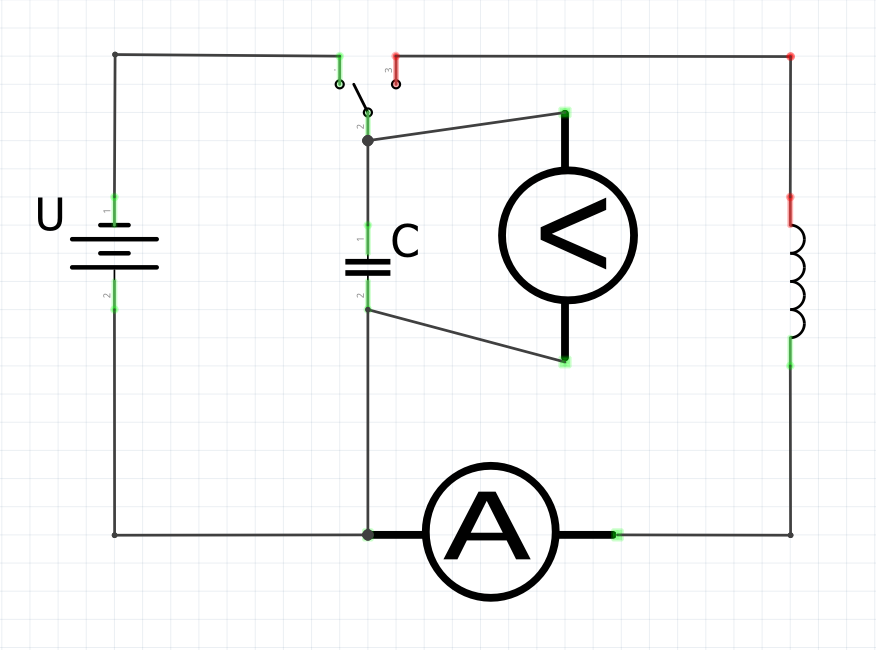
\includegraphics[scale=0.5]{Schwingkreis1}
			
			\subsubsection{Herleitung der physikalischen Gesetze des Schwingkreises}
			
			\begin{itemize}
				\item Wdh. mech. Schwingung: \\
					Kraftgesetz: Die Federkraft ist der Elongation s proportional: \\
					$ \Rightarrow F_R = -D \ast s $ \\
					Kräftegleichung: \\
					$ m \ast a_{(t)} = -D \ast s_{(t)} $ \\
					Differentialgleichung: \\
					$ m \ast \ddot{s}_{(t)} = -D \ast s_{(t)} $ \\
					$ \ddot{s}_{(t)} = -\frac{D}{m} \ast s_{(t)} $ \\
					Lösungsfunktion: $ s_{(t)} = \hat{s} \ast sin(\omega \ast t) $ \\
					\hspace{24mm} mit $ \omega = \sqrt{\frac{D}{m}} $
					
				\item Analog im elektromagnetischen Fall: \\
					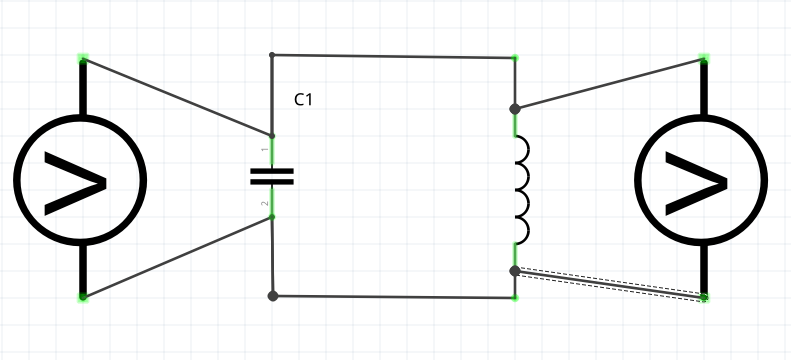
\includegraphics[scale=0.4]{Schwingkreis2} \\
					$ U_{C_{(t)}} = \frac{Q_{(t)}}{C}$ \hspace{21mm}Links \\
					$ U_{ind_{(t)}} = -L \ast \dot{I}_{(t)} $ \hspace{10mm}Rechts \\
					Spannungsgleichung: \\
					$ U_{C_{(t)}} = U_{ind_{(t)}} $ \\
					$ \frac{Q_{(t)}}{C} = -L \ast \dot{I}_{(t)} $ \\
					Differentialgleichung: \\
					$ \dot{I}_{(t)} = -\frac{1}{L \ast C} \ast Q_{t} $ \\
					$ \ddot{Q}_{(t)} = -\frac{1}{L \ast C} \ast Q_{(t)} $ \\
					$ Q_{(t)} = \hat{Q} \ast sin(\omega \ast t + \varphi) $ \\
					mit $ \omega = \sqrt{\frac{1}{L \ast C}} $ \\
			\end{itemize}
			
			\subsubsection{Merke:}
			
			Aus der Spannungsgleichung erhält man im elektromagnetischen Schwingkreis $ \omega = \sqrt{\frac{1}{L \ast C}} $ und $ T = \frac{2\pi}{\omega} = \frac{2\pi}{\sqrt{\frac{1}{L \ast C}}} = 2\pi \ast \sqrt{L \ast C}$ (thomson'sche Schwingungsgleichung)
	\chapter{Klasse12}
	\section{Schwingungskreis}
\subsection{Wdh. Kondensator}
\subsection{EES im Schwingkreis}
$W_{ges}$ ist zeitlich konstant:
\begin{align*}
	\dfrac{1}{2}L*I(t)^2+\dfrac{1}{2}*C*U(t)^2&=konst&&|()'\\
	L*I(t)*I'(t)+C*U(t)*U'(t)&=0&&|U=-L*I'\\
	L*I(t)*I'(t)+C*(-L*I'(t))*U'(t)&=0\\
	I'(t)*L*\left(I(t)-C*\dfrac{Q'(t)}{C}\right)&=0
\end{align*}
\subsection{Vgl. von Schwingkreis mit mech. Schwingung}
\begin{align*}
	U_L&=U_C\\
	-L*I'(t)&=\dfrac{Q(t)}{C}\\
	-L*Q''(t)&=\dfrac{1}{C}*Q(t)\\
	L*Q''(t)+\dfrac{1}{C}*Q(t)&=0&&|\mathrm{DGL\ des\ Schwingkreis}\\
	m*s''(t)+D*s(t)&=0&&|\mathrm{DGL\ der\ mech.\ Schwingung}\\
\end{align*}
\begin{tabular}{l|l}
	SK & MSchw.\\
	\hline $L$&$m$\\
	$\frac{1}{C}$&$D$\\
	$Q$&$s$\\
	$Q'=I$&$v=s'$\\
	$I'$&$a=s''$\\
	$-\frac{1}{C}*Q=-U_C$&$-D*s(t)=F_R$\\
	$-L*I'(t)$ &$-m*a(t)$\\
	$\frac{1}{2}*L*I^2$&$\frac{1}{2}*m*v^2$\\
	$\frac{1}{2}*\frac{1}{C}*Q(t)^2=\frac{1}{2}*C*U(t)^2$&$\frac{1}{2}*D*s^2$	
\end{tabular}

\subsection{Wdh. Energieerhaltungssatz der Mechanik}
\begin{align}
	F(t)&=m*a(t)&&|*v(t)\\
	F(t)*v(t)&=m*a(t)*v(t)\\
	F(t)*v(t)&=m*v'(t)*v(t)&&|\int \mathrm{d}t\\
	\int F(t)*s'(t)\mathrm{d}t&=\int m*v'(t)*v(t)\mathrm{d}t\\
	-\int V'(s(t))*s'(t)\mathrm{d}t&=\int m*v'(t)*v(t)\mathrm{d}t\\
	-V'(s(t))+c_1&=\dfrac{1}{2}*m*v(t)^2+c_2\\
	c&=\dfrac{1}{2}*m*v(t)^2+V'(s(t))\\
	const&=E_{kin}+E_{pot}
\end{align}
Der Energieerhaltungssatz ist nur dann erfüllt, wenn es eine Funktion gibt, für die gilt: \[-V'(s)=F\]

\subsection{Maxwellgleichungen}
\begin{subequations}
	\begin{align}
	\underbrace{\vec{\nabla}}_{\mathrm{Quelle\ von}}\ast\vec{E}=\dfrac{\sigma}{\epsilon_0}&&|\vec{\nabla}=\begin{pmatrix}\partial x\\\partial y\\\partial z\end{pmatrix}\\
	\vec{\nabla} \ast\vec{B}=0\\
	\underbrace{\vec{\nabla} \times}_{\mathrm{Wirbel\ von}} \vec{E}=-\dfrac{\partial B}{\partial t}&&|\mathrm{ Minus\ wegen\ Lenz}\\
	\vec{\nabla} * \vec{B}=\mu_0*J+\mu_0*\epsilon_0*\dfrac{\partial E}{\partial t}
	\end{align}
\end{subequations}
Im Vakuum sind (a) und (b) symmetrisch. (c) und (d) sind ebenfalls symmetrisch.
\begin{subequations}
	\begin{align}
		\vec{\nabla}\ast\vec{E}&=\dfrac{\sigma_e}{\epsilon_0}\\
		\vec{\nabla}\ast\vec{B}&=\mu_0*\sigma_m\\
		\vec{\nabla}\times \vec{E}=-\mu_0*J_m-\dfrac{\partial B}{\partial t}\\
		\vec{\nabla} \times \vec{B}=\mu_0*J_e+\mu_0\epsilon_0\dfrac{\partial E}{\partial t}	
	\end{align}
\end{subequations}



	\chapter*{Disclaimer}
	\section*{Disclaimer}
	Erstellt von Lucca Kümmerle, Patrick Müller und Josua Kugler nach Aufschrieben von Andreas Lörincz bzw. Dr. Susanne Rieseberg. \\ Für Fehler wird keine Haftung übernommen. \\ Alle Rechte liegen bei Lucca Kümmerle, Patrick Müller, Josua Kugler, Andreas Lörincz und Dr. Susanne Rieseberg. \\ Es ist verboten, dieses Dokument ohne die Zustimmung mindestens einer der fünf genannten Personen zu vervielfältigen. \\
	Version: \today
\end{flushleft}
\end{document}